%% This is the ctufit-thesis example file. It is used to produce theses
%% for submission to Czech Technical University, Faculty of Information Technology.
%%
%% This is version 1.6.0, built 18. 9. 2025.
%% 
%% Get the newest version from
%% https://gitlab.fit.cvut.cz/theses-templates/FITthesis-LaTeX
%%
%%
%% Copyright 2024, Tomas Novacek
%% Copyright 2021, Eliska Sestakova and Ondrej Guth
%%
%% This work may be distributed and/or modified under the
%% conditions of the LaTeX Project Public License, either version 1.3
%% of this license or (at your option) any later version.
%% The latest version of this license is in
%%  https://www.latex-project.org/lppl.txt
%% and version 1.3 or later is part of all distributions of LaTeX
%% version 2005/12/01 or later.
%%
%% This work has the LPPL maintenance status `maintained'.
%%
%% The current maintainer of this work is Tomas Novacek (novacto3@fit.cvut.cz).
%% Alternatively, submit bug reports to the tracker at
%% https://gitlab.fit.cvut.cz/theses-templates/FITthesis-LaTeX/issues
%%
%%

% arara: xelatex
% arara: biber
% arara: xelatex
% arara: xelatex

%%%%%%%%%%%%%%%%%%%%%%%%%%%%%%%%%%%%%%%%%
% CLASS OPTIONS
% language: czech/english/slovak
% thesis type: bachelor/master/dissertation/doctoral-report
% electronic (oneside) or printed (twoside), twoside is default
% paragraph - if passed, this optional argument sets paragraphs as the deepest level of headers, styles it, numbers it and adds it to Table of Content. Use with care! Normally, it is considered unwise to use it, since it is too deep.
% colour: bw for black&white OR no option for default colour scheme
%%%%%%%%%%%%%%%%%%%%%%%%%%%%%%%%%%%%%%%%%
\documentclass[english,master,oneside]{ctufit-thesis}

%%%%%%%%%%%%%%%%%%%%%%%%%%%%%%%%%%
% FILL IN THIS INFORMATION
%%%%%%%%%%%%%%%%%%%%%%%%%%%%%%%%%%
\ctufittitle{GPU implementation of acceleration data structures for ray tracing}
\ctufitauthorfull{Bc. Jakub Votrubec}
\ctufitauthorsurnames{Votrubec}
\ctufitauthorgivennames{Jakub}
\ctufitsupervisor{doc. Ing. Ivan Šimeček, Ph.D.}
\ctufitdepartment{Department of Computer Systems}
\ctufitprogram{Informatics}
\ctufitspecialisation{Computer Systems and Networks}
\ctufityear{2026}
\ctufitdeclarationplace{Prague}
\ctufitdeclarationdate{\today}
\ctufitabstractCZE{Tato diplomová práce se zabývá studiem, implementací a vyhodnocením akceleračních datových struktur implementovaných na GPU pro GPU trasování paprsků, se zaměřením na hierarchie obálek (BVH). Teoretická část uvádí základy trasování paprsků, metody konstrukce BVH, algoritmy průchodu hierarchií a vybrané současné přístupy pro zlepšení efektivity konstrukce a vykreslování.

Na tomto základě byly implementovány vybrané algoritmy konstrukce BVH v jazyce CUDA, konkrétně Parallel Locally Ordered Clustering, Extended Morton Codes a Skewed Oriented Bounding Boxes, včetně jejich kombinací. Implementace je navržena jako konfigurovatelné GPU rozhraní, která umožňuje volbu různých variant BVH a parametrů vykreslování.

Pro účely testování byl použit Whitted styl trasování paprsků. Systém je implementován v jazycích C++20 a CUDA 12 a jeho součástí je detailní měření dat během konstrukce BVH i průchodu hierarchií. Rozhraní umožňuje deatilnou analýzu jednotlivých fází.

Experimentální vyhodnocení bylo provedeno na dvou GPU platformách (NVIDIA RTX 3060 Mobile a RTX 4080). Výsledky ukazují, že varianty založené na SOBB snižují počet testů průsečíku paprsku s primitivy díky těsnějším ohraničujícím obálkám, což zlepšuje efektivitu průchodu hierarchií, avšak pouze ve vhodných scénách, ve většině testovaných scén naopak zhoršují průchod a výrazně zvyšují čas konstrukce a zhoršují efektivitu trasování paprsků. Varianty EMC nezvyšují významně čas konstrukce, avšak májí pouze minimální pozitivní vliv na průchod hierarchií a trasování pro většinu testovaných scén.

Výsledky ukazují kompromisy mezi výpočetní náročností konstrukce BVH a efektivitou průchodu hierarchií pro různé akcelerační datové struktury.}
\ctufitabstractENG{This thesis focuses on the study, implementation, and evaluation of acceleration data structures implemented on the GPU for GPU-based ray tracing, with emphasis on bounding volume hierarchies (BVH). The theoretical part introduces ray tracing fundamentals, BVH construction techniques, traversal methods, and selected state-of-the-art approaches for improving construction efficiency and rendering performance.

Based on this foundation, several BVH construction algorithms were implemented in CUDA, including Parallel Locally Ordered Clustering, Extended Morton Codes, and Skewed Oriented Bounding Boxes, as well as their combinations. The implementation is designed as a configurable GPU pipeline that allows selection of different BVH variants and rendering parameters.

A Whitted-style ray tracing framework is used for evaluation. The system is implemented in C++20 and CUDA 12 and includes detailed instrumentation for measuring performance during both BVH construction and ray traversal. The framework enables fine-grained analysis of individual pipeline stages.

Experimental evaluation was performed on two GPU platforms (NVIDIA RTX 3060 Mobile and RTX 4080). The results show that SOBB-based variants reduce the number of ray-primitive intersection tests due to tighter bounding volumes, improving traversal efficiency but only in suitable scenes, in the majority of tested scenes they hinder the traversal efficiency and lead to significantly higher build times. EMC-based variants do not significantly increasing construction time, but also increase the traversal performance only marginally for the majority of tested scenes.

The results demonstrate the trade-off between BVH construction cost and traversal efficiency across different acceleration structure designs.}
\ctufitkeywordsCZE{Masivně paralelní algoritmy, Výpočetní geometrie, Řazení a vyhledávání, Hierarchie obálek, Vrhání paprsků}
\ctufitkeywordsENG{Massively parallel algorithms, Computational geometry, Sorting and searching, Bounding volume hierarchy, Ray tracing}
%%%%%%%%%%%%%%%%%%%%%%%%%%%%%%%%%%
% END FILL IN
%%%%%%%%%%%%%%%%%%%%%%%%%%%%%%%%%%

%%%%%%%%%%%%%%%%%%%%%%%%%%%%%%%%%%
% CUSTOMIZATION of this template
% Skip this part or alter it if you know what you are doing.
%%%%%%%%%%%%%%%%%%%%%%%%%%%%%%%%%%

\RequirePackage{iftex}[2020/03/06]
\iftutex % XeLaTeX and LuaLaTeX
    \RequirePackage{ellipsis}[2020/05/22] %ellipsis workaround for XeLaTeX
\else
    \errmessage{Only compilation with XeLaTeX or LuaLaTeX is allowed}
    \stop
\fi

% hyperlinks
\hypersetup{
    pdfpagelayout=SinglePage,
    colorlinks=false,
    allcolors=decoration,
    pdfborder={0 0 0.1}
}

% uncomment the following to hide all hyperlinks
%\hypersetup{hidelinks}

% uncomment the following to change the colour of all hyperlinks to CTU blue
%\hypersetup{allbordercolors=decoration}

\RequirePackage{pdfpages}[2020/01/28]

%%%%%%%%%%%%%%%%%%%%%%%%%%%%%%%%%%
% CUSTOMIZATION of this template END
%%%%%%%%%%%%%%%%%%%%%%%%%%%%%%%%%%


%%%%%%%%%%%%%%%%%%%%%%
% PACKAGES SETTINGS
% You may choose to modify this part.
%%%%%%%%%%%%%%%%%%%%%%
\usepackage{dirtree}
\usepackage{lipsum,tikz}
\usepackage[style=iso-numeric]{biblatex}
\addbibresource{text/bib-database.bib}
\usepackage{xurl}
\usepackage{listings}
\usepackage{minted}
\usepackage{csquotes}
\usepackage{amsmath}

\usepackage{multirow}
\usepackage{graphicx}
\usepackage{algorithm}
\usepackage{algpseudocode}
% Right-aligned line comments
\algrenewcommand{\algorithmiccomment}[1]{\hfill$\triangleright$~#1}
% Hide block endings
\algtext*{EndIf}
\algtext*{EndFor}
\algtext*{EndWhile}
\algtext*{EndFunction}
\usepackage{xcolor}
\usepackage{subcaption}


%%%%%%%%%%%%%%%%%%%%%%
% PACKAGES SETTINGS END
%%%%%%%%%%%%%%%%%%%%%%

\begin{document}
\frontmatter\frontmatterinit % do not remove these two commands

\thispagestyle{empty}\maketitle\thispagestyle{empty}\cleardoublepage % do not remove these four commands

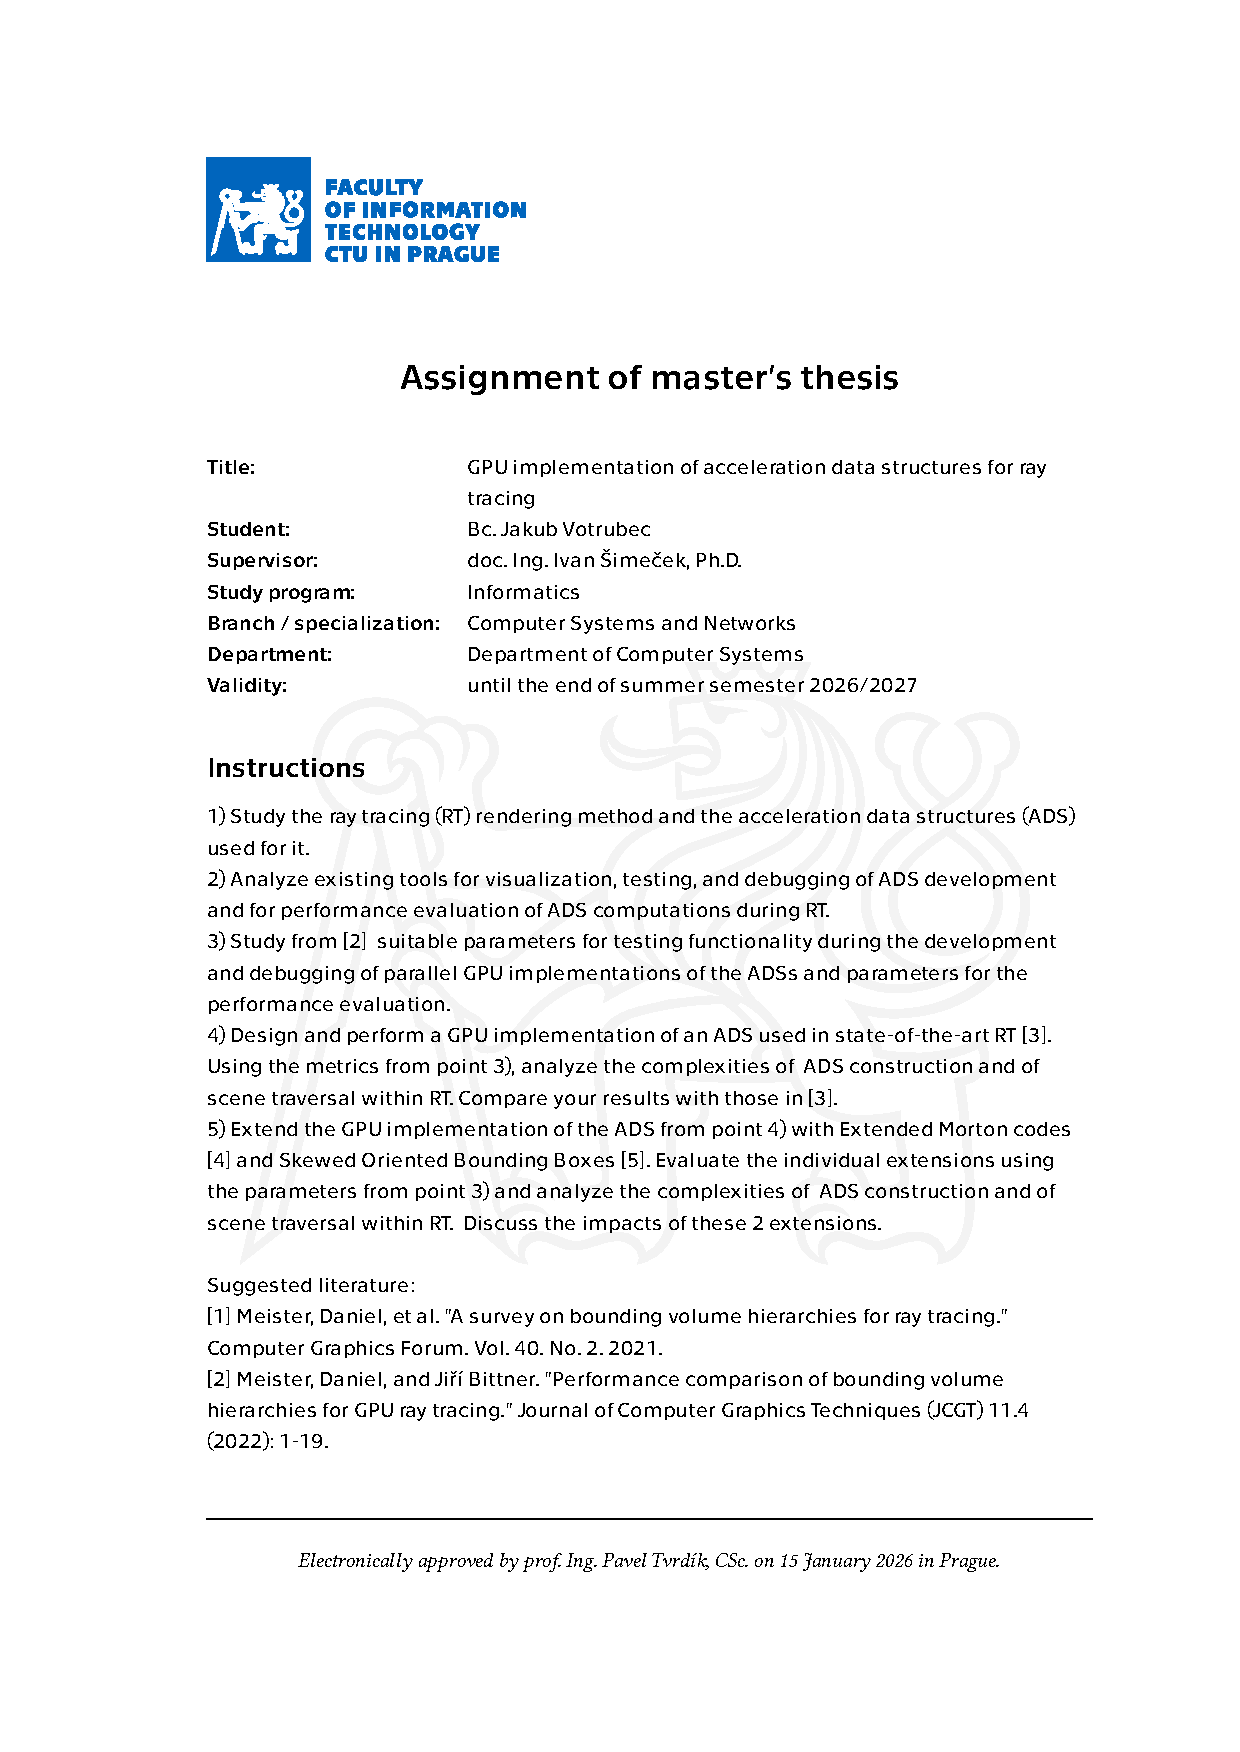
\includepdf[pages={1-}]{votruja6-assignment.pdf}

\imprintpage % do not remove this command
\stopTOCentries

%%%%%%%%%%%%%%%%%%%
% ACKNOWLEDGMENT
% FILL IN / MODIFY
% This is a place to thank people for helping you. It is common to thank your supervisor.
%%%%%%%%%%%%%%%%%%%
\begin{acknowledgmentpage}
First and foremost I would like to thank my supervisor for his help, patience and constructive criticism that he showered me with throughout the whole thesis. Next I need to thank my family for supporting me during my studies and always being there for me, even during trying times. Last but not least I would like to express my thanks to my friends that have made my university years one of the greatest and most memorable parts of my life.
\end{acknowledgmentpage}
%%%%%%%%%%%%%%%%%%%
% ACKNOWLEDGMENT END
%%%%%%%%%%%%%%%%%%%


%%%%%%%%%%%%%%%%%%%
% DECLARATION
% FILL IN / MODIFY
%%%%%%%%%%%%%%%%%%%
% INSTRUCTIONS
% ENG: choose one of approved texts of the declaration. DO NOT CREATE YOUR OWN. Find the approved texts at https://courses.fit.cvut.cz/SFE/download/index.html#_documents (document Declaration for FT in English)
% CZE/SLO: Vyberte jedno z fakultou schvalenych prohlaseni. NEVKLADEJTE VLASTNI TEXT. Schvalena prohlaseni najdete zde: https://courses.fit.cvut.cz/SZZ/dokumenty/index.html#_dokumenty (prohlášení do ZP)
\begin{declarationpage}
I hereby declare that the presented thesis is my own work and that I have cited all sources of information in accordance with the Guideline for adhering to ethical principles when elaborating an academic final thesis.

I acknowledge that my thesis is subject to the rights and obligations stipulated by the Act No. 121/2000 Coll., the Copyright Act, as amended, in particular that the Czech Technical University in Prague has the right to conclude a license agreement on the utilization of this thesis as a school work under the provisions of Article 60 (1) of the Act.

I declare that I have used AI tools during the preparation and writing of my thesis. I have verified
the generated content. I confirm that I am aware that I am fully responsible for the content of the
thesis.
\end{declarationpage}
%%%%%%%%%%%%%%%%%%%
% DECLARATION END
%%%%%%%%%%%%%%%%%%%

% Use one of the two following commands. The first prints abstracts+keywords on two pages, the second puts them on one page (if possible). \printonepageabstract can also accept optional argument that specifies a vertical space before both abstracts (the default is 18 mm).
%\printtwopageabstract
\printonepageabstract 

\tableofcontents % do not remove this command
%%%%%%%%%%%%%%%%%%%%%%
% list of other contents: figures, tables, code listings, algorithms, etc.
% add/remove commands accordingly
%%%%%%%%%%%%%%%%%%%%%%
\listoffigures % list of figures
\begingroup
\let\clearpage\relax
\listoftables % list of tables. Remove if you do not have any.
\thectufitlistingscommand{} % list of code listings. Remove if you do not have any.
\thectufitlistofalgorithmscommand{} % list of algorithm pseudocodes defined using the algorithm package.
\endgroup
%%%%%%%%%%%%%%%%%%%%%%
% list of other contents END
%%%%%%%%%%%%%%%%%%%%%%

%%%%%%%%%%%%%%%%%%%
% ABBREVIATIONS
% FILL IN / MODIFY
% OR REMOVE ENTIRELY
% List the abbreviations in lexicography order.
%%%%%%%%%%%%%%%%%%%
\chapter{\thectufitabbreviationlabel}

\begin{tabular}{rl}
	AABB  & Axis Aligned Bounding Box                      \\
	ADS   & Acceleration Data Structure                    \\
    BVH   & Bounding Volume Hierarchy                      \\
	DOP   & Discrete Oriented Polytope                     \\
	EMC   & Extended Morton Codes                          \\
	GPU   & Graphics Processing Unit                       \\
    LBVH  & Linear Bounding Volume Hierarchy               \\
	OBB   & Oriented Bounding Boxes                        \\
	PLOC  & Parallel Locally Ordered Clustering            \\
	RT    & Ray Tracing                                    \\
	SA    & Surface Area                                   \\
	SAH   & Surface Area Heuristic                         \\
    SIMD  & Single Instruction Multiple Data               \\
	SOBB  & Skewed Oriented Bounding Box
\end{tabular}
%%%%%%%%%%%%%%%%%%%
% ABBREVIATIONS END
%%%%%%%%%%%%%%%%%%%
\resumeTOCentries
\mainmatter\mainmatterinit % do not remove these two commands
%%%%%%%%%%%%%%%%%%%
% THE THESIS
% MODIFY ANYTHING BELOW THIS LINE
%%%%%%%%%%%%%%%%%%%

%---------------------------------------------------------------
\chapter{Introduction} %\addcontentsline{toc}{chapter}{Introduction}\markboth{Introduction}{Introduction}
%---------------------------------------------------------------
\setcounter{page}{1}

Ray tracing is a physically based method for realistic image synthesis that simulates the propagation of light in a 3D scene. By tracing rays and evaluating their interactions with geometry and materials, it enables effects such as reflections and refractions. However, the large number of rays required for high-quality rendering makes ray tracing computationally expensive.

Modern GPUs provide massive parallelism, making them well suited for ray tracing workloads. To fully utilize their capabilities, efficient spatial acceleration structures are required to reduce the number of ray-primitive intersection tests. Among these, bounding volume hierarchies (BVHs) are widely used due to their favorable balance between construction cost and traversal efficiency.

This thesis focuses on BVHs and their efficient construction and traversal on GPU architectures. In particular, it investigates how different construction strategies and bounding volume representations influence traversal performance. The work builds upon three selected approaches: Parallel Locally-Ordered Clustering \cite{MB17}, Extended Morton Codes \cite{Vinkler2017}, and Skewed Oriented Bounding Boxes \cite{KB25}. In addition to evaluating these methods individually, their combinations are explored within a unified framework.

The main contribution of this thesis will be the implementation and experimental evaluation of these approaches on modern GPUs. The methods will be compared using a consistent set of metrics, including construction time, traversal performance, and BVH cost. Furthermore, the thesis will analyze the relationship between theoretical quality metrics and actual runtime behavior, highlighting the influence of hardware-dependent factors.

The thesis will be structured as follows. Chapter~\ref{chap:theory} will introduce the theoretical background of ray tracing and acceleration structures. Chapter~\ref{chap:measurement} will be an introduction to the methodology of testing the acceleration data structures. Chapter~\ref{chap:implementation} will describe the implementation of the selected methods, including data structures and GPU-specific considerations. Chapter~\ref{chap:results} will present the experimental setup and evaluation results, followed by their analysis. Finally, Chapter~\ref{chap:conclusion} will summarize the findings and outline directions for future work.

\section{Goals}

The primary goal of this thesis is to implement and compare selected BVH construction techniques and their extensions on GPU architectures. This includes methods proposed by Meister et al.~\cite{MB17}, Vinkler et al.~\cite{Vinkler2017}, and Káčerik et al.~\cite{KB25}, as well as their combinations.

A secondary goal is to establish a consistent experimental framework for evaluating BVH performance. The evaluation is based on metrics such as construction time, traversal performance, and BVH cost, following the methodology of Meister et al.~\cite{MB22}.

The final objective is to analyze the relationship between structural BVH quality metrics and actual ray tracing performance, and to identify the most effective approaches and combinations for practical use.


% chapter Ray tracing and Abstract data structures
%---------------------------------------------------------------
\chapter{Ray tracing and acceleration data structures}
\label{chap:theory}
%---------------------------------------------------------------

\begin{chapterabstract}
 
This chapter focuses on exploring ray tracing and acceleration data structures used for ray tracing. In particular it will delve into bounding volume hierarchies, starting from the theoretical foundations of cost functions, construction methods and traversal all the way to specific research papers focused on enhancing and expanding the existing techniques. The main goal of this chapter is to enrich the reader and welcome him into the topic of bounding volume hierarchies. Special focus will be given to GPU friendly algorithms and techniques.

\end{chapterabstract}

\begin{figure}[h!tb]
    \centering
    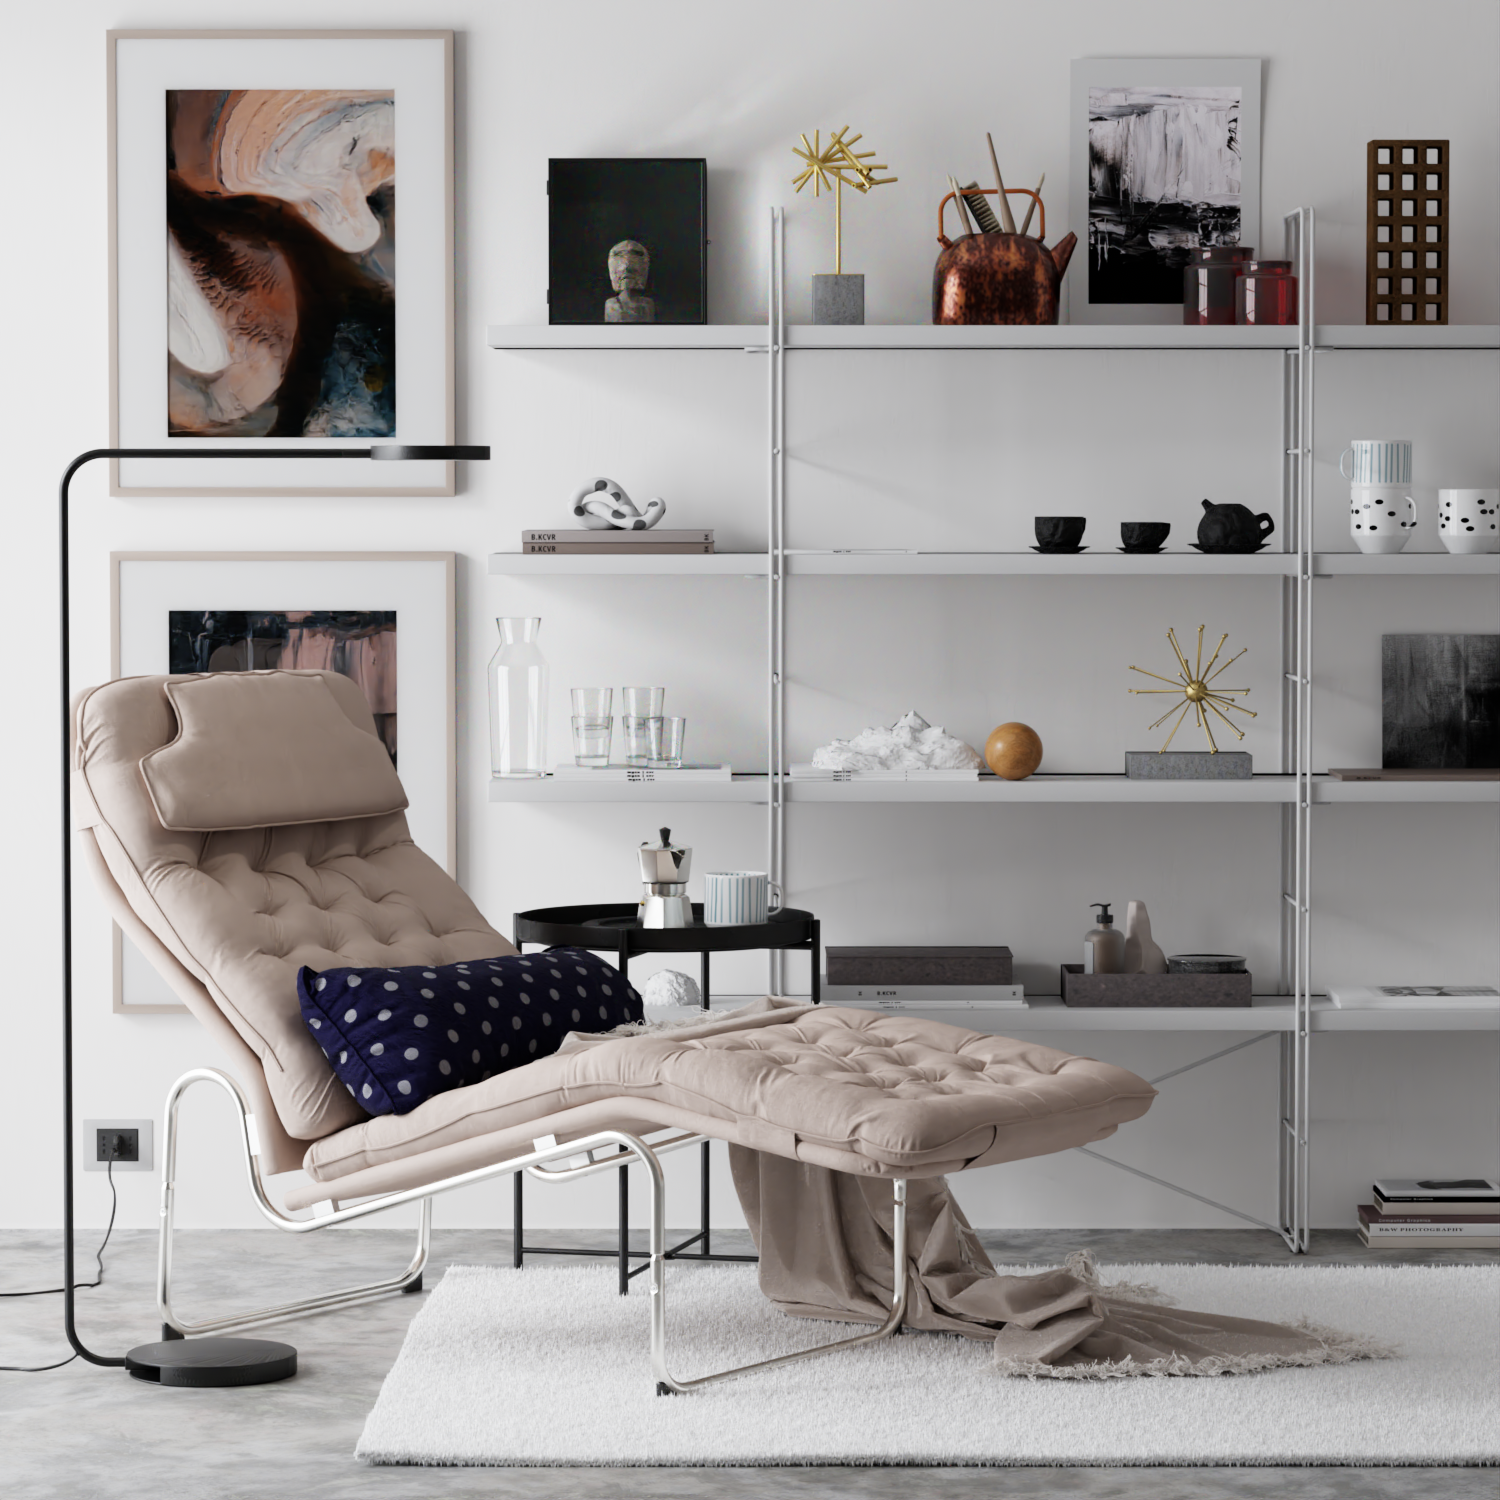
\includegraphics[width=0.95\textwidth]{images/pbr renders/fancy_render_pbr2.png}
    \caption{Rendering capabilities of ray tracing. Courtesy of the PBR book \cite{pbr4}}
    \label{fig:pbr4_render}
\end{figure}

\section{Ray tracing}

Ray tracing is a physically based rendering technique used to render images by simulating the propagation of light in a scene made up of primitives (typically triangles). The fundamental idea is to trace rays from the camera through each pixel into the scene, finding their interactions with geometry and materials. Compared to traditional rasterization methods, ray tracing naturally supports effects such as reflections, refractions, and shadows, making it particularly suitable for realistic image synthesis. Figure \ref{fig:pbr4_render} shows the capabilities of this rendering technique.

A basic approach to ray tracing was introduced by Whitted~\cite{W80}, who proposed a recursive algorithm for handling reflection and refraction. In this model, primary rays are cast from the camera into the scene to determine visible surfaces. At each intersection point, additional rays are generated to simulate reflected and refracted light, as well as shadow rays to determine the visibility of light sources (if the intersection point receives energy from them). This recursive process enables the simulation of complex optical effects, although it is limited in its ability to model diffuse global illumination.~\cite{W80}

A more general formulation of light transport is given by the rendering equation, introduced by Kajiya~\cite{K86}. The rendering equation expresses the outgoing radiance at a point as the sum of emitted and reflected radiance over all incoming directions. It is defined as~\cite{K86}:
\begin{equation}
L_o(x, \omega_o) = L_e(x, \omega_o) + \int_{\Omega} f_r(x, \omega_i, \omega_o) \, L_i(x, \omega_i) \, (\omega_i \cdot n) \, d\omega_i,
\end{equation}
where $L_o$ is the outgoing radiance, $L_e$ is the emitted radiance, $f_r$ is the bidirectional reflectance distribution function (BRDF), and $L_i$ is the incoming radiance. The integral is taken over the hemisphere $\Omega$ above the surface point. This equation provides a physically accurate description of light transport but does not have a closed-form solution in the general case, requiring numerical approximation methods such as Monte Carlo integration.~\cite{K86}

The high computational complexity of ray tracing stems from the need to evaluate ray-scene intersections for a large number of rays. For a scene consisting of $N$ geometric primitives, a naive ray tracing approach requires testing each ray against all primitives, resulting in $O(N)$ intersection tests per ray. Since realistic rendering requires tracing millions to billions of rays, the overall complexity becomes unbearable. Furthermore, recursive ray generation (e.g., for reflections and global illumination) increases the number of rays exponentially with recursion depth.

To address this issue, acceleration data structures (ADS), such as bounding volume hierarchies (BVH), are employed to reduce the number of intersection tests. These structures divide the scene geometry in a hierarchical manner (either by dividing space or objects), allowing large groups of primitives to be culled with a single intersection test. As a result, the expected complexity of ray traversal can be reduced to approximately $O(\log N)$ for well-constructed hierarchies, making ray tracing feasable for complex scenes.

The challenges of ray tracing are further amplified on modern parallel architectures such as GPUs. The irregular memory access patterns, control flow divergence, and varying workloads per ray complicate efficient parallel implementation. In particular, traversal of hierarchical data structures such as BVHs introduces branch divergence and incoherent memory access, which can significantly degrade performance. These challenges motivate the development of specialized data structures and algorithms optimized for GPU execution, which are the focus of this thesis.

% ----------------------------------------
\newpage
\clearpage
\section{Acceleration data structures}
% - Základní typy datových struktur používaných pro ray tracing

\begin{figure}[h!tb]
    \centering
    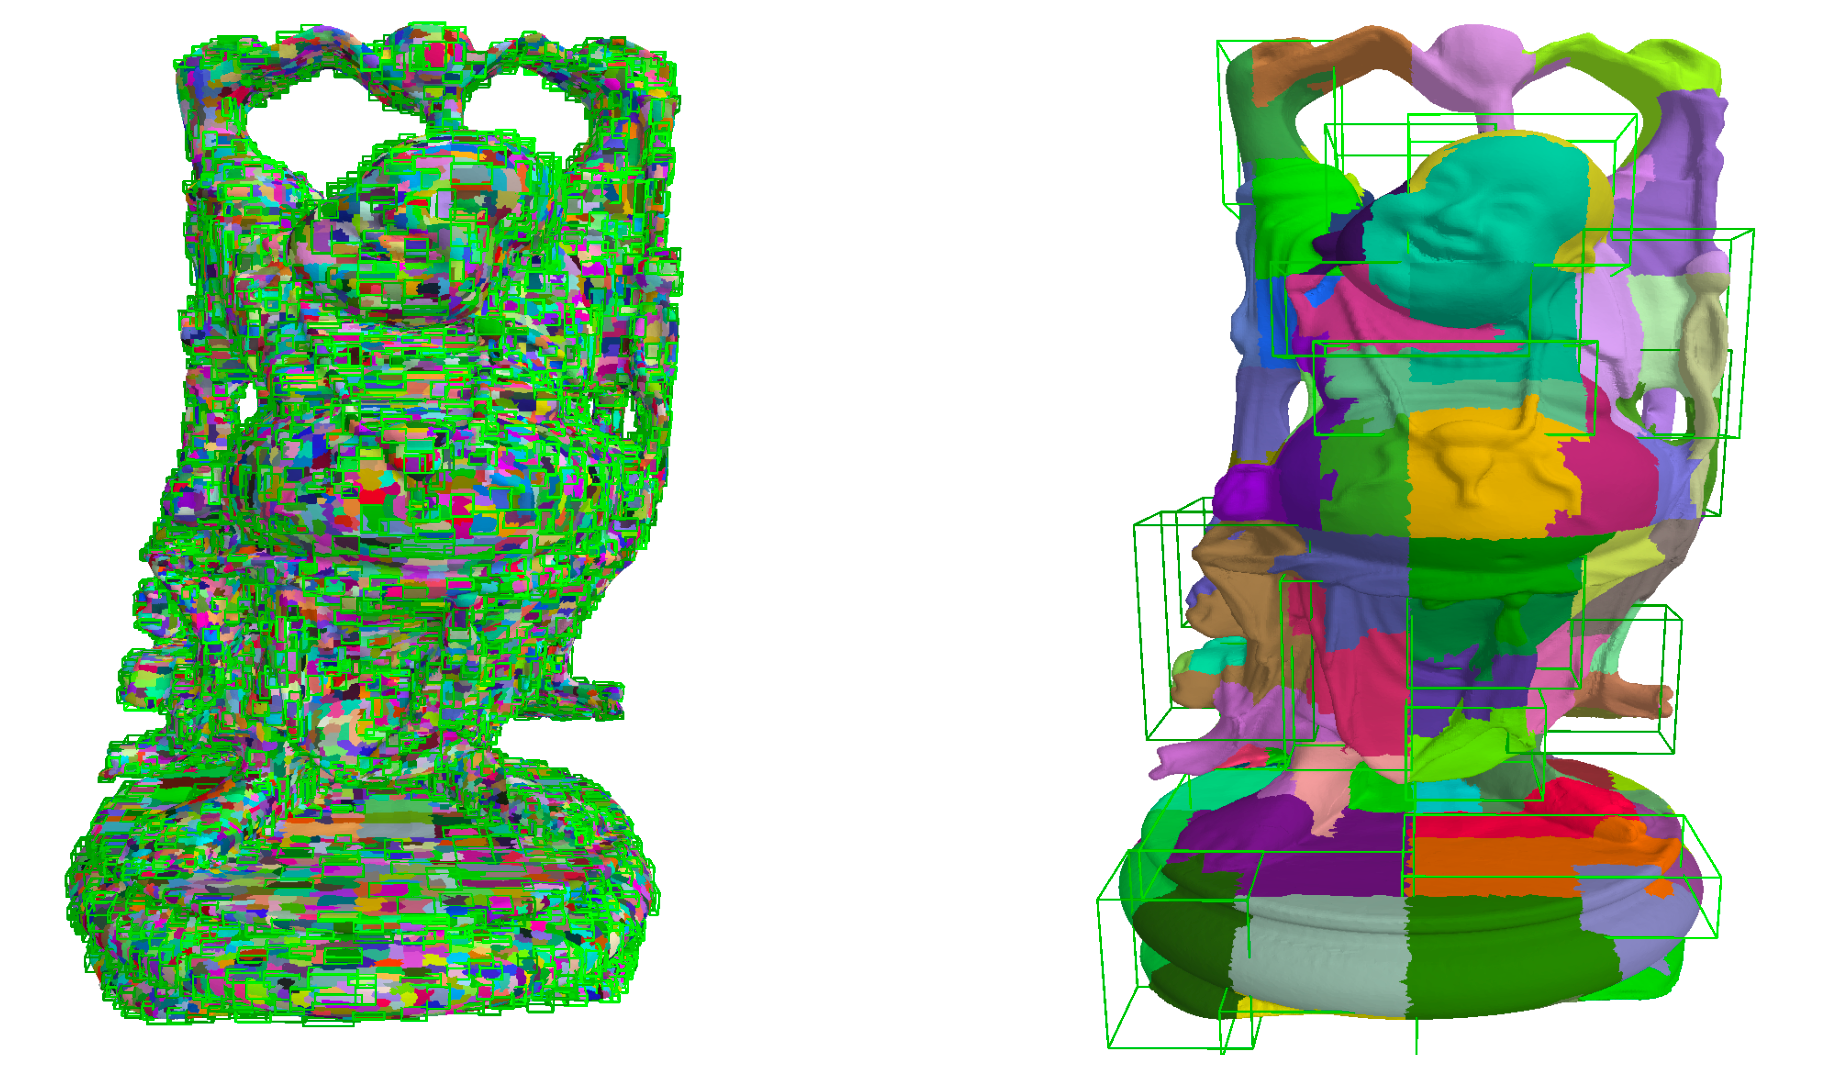
\includegraphics[width=0.95\textwidth]{images/BVH_visualisation_PLOC.png}
    \caption{Visualization of the different stages of BVH construction. \cite{MB17}}
    \label{fig:ploc_clusterint_example}
\end{figure}

The problem of realistic image synthesis using ray tracing is the sheer number of rays needed that must be traced to get plausible results. Otherwise, the resulting images are plagued with high-frequency noise. The light transport simulation is based on a basic geometric operation, \textit{finding the nearest intersection} of a given ray with the scene. We might also want to find \textit{any intersection} or \textit{all intersections} with the scene. The query into the scene is usually described as a \textit{ray} with an \textit{origin} and a \textit{direction}. Without any optimizations, we would have to compute the ray-scene intersections one by one for each ray-primitive pair. This becomes computationally unfeasible very quickly as scenes might consist of millions of primitives, and the number of rays is at least as large as the number of pixels in the desired image. \cite{Meister2021}

The simulation of light transport can be accelerated, for example, by sorting scene primitives into efficient spatial data structures, namely acceleration data structures. In the last decades, the most popular acceleration data structure for ray tracing is the bounding volume hierarchy \cite{Cla76}. For that reason, this section will focus on it in favor of other ADS.

This thesis will focus on the bounding volume hierarchy data structures that are used for ray tracing. There are many other data structures used for ray tracing, but over the years BVH has become the de facto industry standard when it comes to ray tracing acceleration. 

Other data structures include, for example, Octrees that were first introduced in 1982 \cite{M82} and first used for ray tracing in 1984 \cite{G84} and KD-trees that were first introduced in 1975 \cite{B75} and first used for ray tracing in 1990 \cite{MB90} using the surface area heuristic \cite{GS87} (more on this later). However, these data structures are not within the scope of this thesis.

\subsection{Bounding volume hierarchy}
A \textit{bounding volume hierarchy} is a rooted tree with a branching factor (denoted \textit{k}). Individual nodes have two types: interior nodes, which hold pointers to child nodes, and leaf nodes, which hold references to scene primitives. All nodes contain a bounding volume that tightly wraps around the geometry in the leaves. BVH was originally a binary tree, but in recent years a higher branching factor has become favorable. In the context of ray tracing, the bounding volume of choice is almost exclusively an \textit{axis aligned bounding box} (AABB). It is used for its small memory footprint and computationally easy intersection with rays. Other bounding volumes are sometimes used for specific cases. For example, \textit{bounding spheres}, \textit{oriented bounding boxes} (OBB), or, more recently, more experimental \textit{skewed oriented bounding boxes} (SOBB) — more on them in a later Section \ref{sec:sobb} — are being used. BVH can theoretically be used with an arbitrary number of dimensions, but in rendering, where scene primitives are 3D entities, more than 3 dimensions are rarely needed.

The popularity of BVHs comes from the following advantages:

\paragraph{Predictable memory footprint} The number of primitives directly influences the memory footprint. Scene primitives are usually referenced only once. In that case, the BVH is made up of at most $2n-1$ nodes (where $n$ is the number of primitives). This corresponds to a binary BVH with a single primitive in each leaf. If the branching factor \textit{k} is higher, the number of internal nodes decreases. The same applies, but for leaf nodes, when more than one primitive is stored in a single leaf node. \cite{Meister2021}

\paragraph{Robust and efficient query} Due to the hierarchical structure and the use of objects instead of spatial splitting, the BVH is robust to any scene distribution. For example, the \textit{"teapot in the stadium problem"}\footnote{ is a very small and detailed object inside a large object — a vast difference in scale can lead to poor splitting.}. Using spatial splitting data structures, we would not cull the space efficiently enough, but using BVH, we are able to efficiently prune branches when traversing the tree and quickly get rid of the branches that do not intersect a given ray. BVH traversal algorithms typically have a small and compact traversal state and can be efficiently parallelized \cite{Meister2021}. This results in great ray tracing performance, in most cases at least as good as KD-trees \cite{VHB16}, taking their place as the best data structure for ray tracing \cite{Hav00}.

\paragraph{Scalable construction} Various construction algorithms for BVH exist, ranging from very fast to complex algorithms, providing high quality results in exchange for longer build times. With this flexibility, we can tailor the balance to our needs between construction speed and BVH quality. The most straightforward metric for BVH quality in the field of ray tracing is the speed in millions of rays cast per second (MRays/s). We usually optimize the total time to render the image, which is the sum of the ray casting and the constuction time. In real-time applications, we usually have a small budget for both these phases, thus we have to limit ourselves to a medium quality BVH in exchange for faster construction. This works because the number of rays that can be cast is lower and it is not worth investing more time into constructing a higher quality BVH. On the other hand, in offline rendering, where the time budget is not as tight, we can afford to invest more time in construction because the number of rays cast is significantly higher than in real-time rendering, yielding a net performance gain. \cite{Meister2021}

\paragraph{Dynamic geometry} Spatial subdivision suffers from the inability to easily refit bounding volumes (such as the KD-tree). Compared to BVH, where the reffitting can be done by a simple bottom up pass. Also, since fast BVH construction methods are available, it is suitable for use with dynamic geometry through straightforward rebuilding. \cite{Meister2021}

\paragraph{}A basic top down construction of BVH can be done recursively by splitting the set of primitives info subsets. The pseudocode is shown in Algorithm \ref{alg:top-down-bvh}.

\begin{algorithm}[h!tb]
\caption{Basic top-down BVH construction algorithm\cite{Meister2021}.}
\label{alg:top-down-bvh}
\begin{algorithmic}[1]
\While{stack is not empty}
    \State pop \textit{node} from the top of the stack
    \If{termination criteria for \textit{node} are met}
        \State make \textit{node} info leaf
    \Else
        \State split primitives in \textit{node} into \textit{children}
        \State assign \textit{children} as child nodes of \textit{node}
        \For{child in node}
            \State push \textit{child} onto the stack
        \EndFor
    \EndIf
\EndWhile
\end{algorithmic}
\end{algorithm}

\paragraph{} To find the nearest neighbor, the BVH can be traversed in a top down manner, starting from the root. A depth-first-search approach is usually used, storing interior nodes in a stack during traversal and traversing first the nodes that potentially contain the nearest intersection. We store the distance to the nearest intersection found so far and cull the nodes that are further. A basic traversal algorithm is illustrated in Figure \ref{fig:bvh-traversal} and its pseudocode is shown in Algorithm \ref{alg:bvh-traversal}.

\begin{figure}[h!tb]
    \centering
    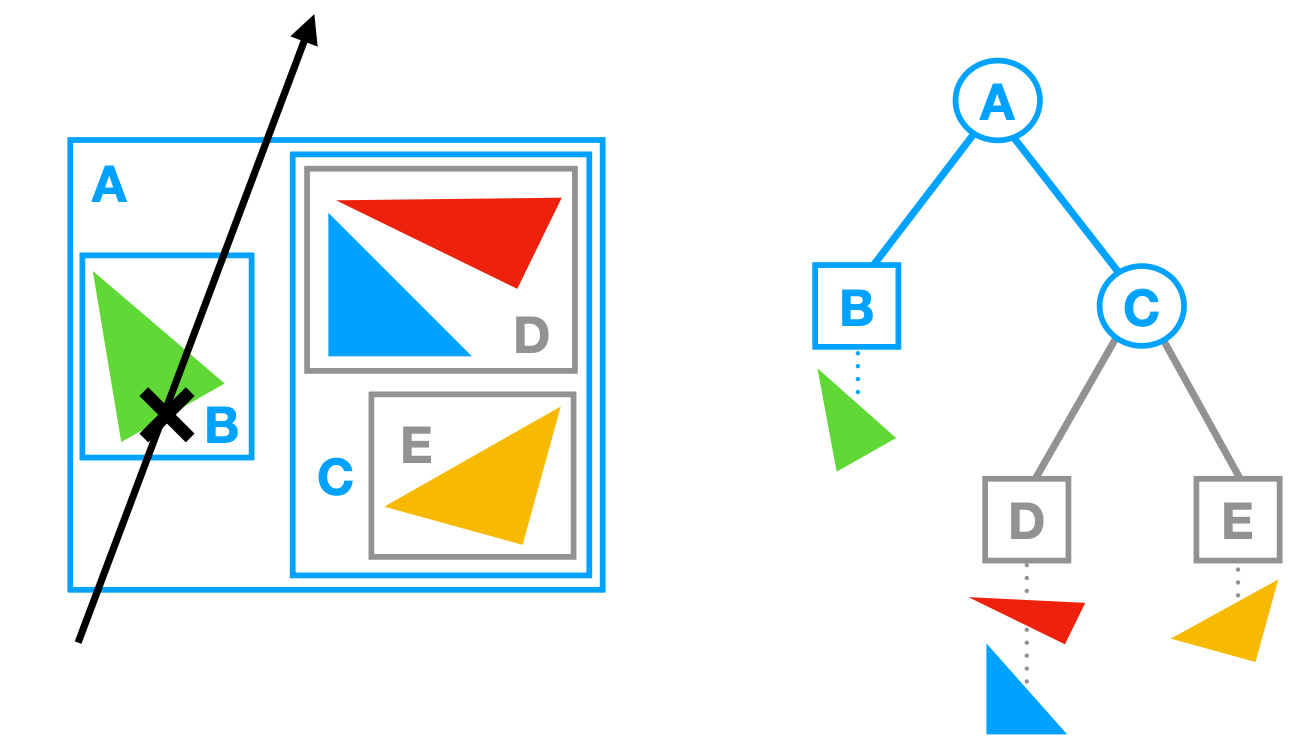
\includegraphics[width=0.9\linewidth]{images/BVHTraversal.png}
    \caption{Example BVH over 4 primitives. Constructed tree includes bounding volumes (AABBs). While traversing the scene we cull the entire subtree of node C since the ray does not intersect its bounding box\cite{Meister2021}.}
    \label{fig:bvh-traversal}
\end{figure}

\begin{algorithm}[h!tb]
\caption{Basic stack-based BVH traversal algorithm\cite{Meister2021}.}
\label{alg:bvh-traversal}
\begin{algorithmic}[1]
\State push \textit{root} onto the stack
\While{stack is not empty}
    \State pop \textit{node} from the top of the stack
    \If{\textit{ray} intersects \textit{node}}
        \If{\textit{node} is not a leaf}
            \For{\textit{child} in \textit{node}}
                \State push \textit{child} onto stack
            \EndFor
        \Else
            \For{\textit{prim} in \textit{node}}
                \State test whether \textit{ray} intersects \textit{prim}
            \EndFor
        \EndIf
    \EndIf
\EndWhile
\end{algorithmic}
\end{algorithm}

\subsubsection{Cost function}
\label{sec:cost-function}

The quality of a BVH can be estimated using a cost function. Cost functions attempt to capture the expected number of operations needed for finding the nearest intersection with a given ray. The cost of a BVH rooted in node $N$ is described by the equation \cite{Meister2021}:
\begin{equation}
    c(N) =
    \begin{cases}
        c_T + \displaystyle\sum_{N_c} P(N_c \mid N) c(N_c) & \text{if } N \text{ is interior node}, \\
        c_I \lvert N \rvert & \text{otherwise},
    \end{cases}
    \label{eq:cost-function}
\end{equation}
where $c(N)$ is the cost of a subtree with root $N$, $N_c$ is a child of $N$, $P(N_c|N)$ is the conditional probability of traversing node $N_c$ when already in node $N$. $|N|$ is then the number of scene primitives in a subtree with root node $N$. The average cost of a traversal step is denoted by $c_T$ and the average cost of a ray-primitive intersection is expressed by $c_I$. The concrete values of these constants are very roughly estimated instead of a precise number of computation steps. In practice, only the ratio of these constants is important, not the absolute values.

\paragraph{Surface area heuristic (SAH) \cite{GS87}} can be used to express conditional probability as geometric probabilities, than means that the ratio of the surface areas of child and parent nodes can be used instead of the conditional probability:
\begin{equation}
    P(N_c \mid N)^{SAH} = \frac{SA(N_c)}{SA(N)},
    \label{eq:sah-conditional-propability}
\end{equation}
where $SA(N)$ denotes the surface area of the bounding volume of node $N$. By substituting Equation \ref{eq:sah-conditional-propability} into Equation \ref{eq:cost-function} and unrolling to remove the recurrence, we get the following:
\begin{equation}
    c(N)^{SAH} = \frac{1}{SA(N)} \left[ c_T \sum_{N_i} SA(N_i) + c_I \sum_{N_l} SA(N_l) |N_l| \right], 
    \label{eq:placeholder_label}
\end{equation}
The problem of finding an optimal BVH is believed to be NP-hard \cite{AK13}.

\paragraph{Other cost functions} exist. The SAH assumes that the rays are uniformly distributed around the scene, with their origins outside. That is unrealistic, and so other cost functions or SAH corrections were suggested. For example, Bittner and Havran \cite{BH09} proposed a method that takes into account the distribution of rays in a scene and then used the ratio of ray hits instead of surface areas, they called it \textit{ray distribution heuristic}. Vinkler et al \cite{VHS12} proposed using the ratio of visible scene primitives, called \textit{occlusion heuristic}. Many more SAH upgrades or completely new methods exist, but that is outside of the scope of this thesis.

\subsubsection{Construction}

In this section, we will summarize the basic construction methods. Basic methods include top-down methods, bottom-up methods, and incremental construction methods. When we already have the BVH tree, it can be transformed or optimized into a wide BVH, for example, by increasing its branching factor by subtree collapsing.

\paragraph{Top-down construction} was adapted from KD-tree construction methods \cite{Wal07}. It starts with the root node that contains the whole scene. In each recursive step, the scene primitives are split into two (or more, based on \textit{k}) disjoint sets that are assigned to the two (or \textit{k}) children of the current node. This continues until the termination conditions are met. The termination conditions usually are the maximum number of primitives in a node/leaf, the maximum depth, or a memory bound. In general, there are exponentially many ways to split scene primitives into disjoint subsets. Even if we perform an optimal split at every step, the final BVH might not be optimal and is very likely to be just a local optimum of the cost function. \cite{Meister2021}

In practice, we split the scene primitives using axis-aligned planes. Each scene primitive is referenced only once, it lives in only one leaf node. We approximate the scene primitive by a single point in space (typically the centroid of the bounding box), of which we can then determine into which disjoint set it belongs. First, we select the best splitting axis either by the spatial median, object median, a cost function, or artificially, such as round-robin or by largest extent. The spatial median splits the bounding box in the middle. The object median selects a splitting point in a way that half of the scene primitives are on each side (this can also be used as a backup splitting method). The cost function split tries to minimize the cost locally, treating the children as leaves.

We can also use the local costs as a termination condition. If the split created has a higher cost than a leaf, we do not split further and create a leaf from the current node.

\paragraph{Bottom-up construction} is an opposite approach to top-down construction by agglomerative clustering \cite{WBKP08}. At first, all scene primitives are clusters of size one. In each iteration, the closest pairs of clusters are merged into larger clusters. The algorithm terminates when there is only one cluster left, the root. The distance of pairs is the surface area of the bounding box that tightly encloses both clusters. In general, agglomerative clustering creates lower cost BVHs, but the construction takes longer. This cost may be deceiving because the optimizations are mostly at the bottom levels of the tree, so, the upper levels might be poorly optimized (unlike in top-down methods). This may lead to worse performance due to the fact that most traversal time is spent in the upper levels. The most expensive part of the method is the nearest neighbor search that has to be done in each iteration for each cluster pair. \cite{Meister2021} 

\paragraph{Incremental construction} works similarly to a heap sort. We start with an empty BVH tree and insert scene primitives one by one. Each primitive is inserted  into an appropriate leaf node that is found by traversing the BVH from the root. If a leaf has too many primitives, it is split into two new leaf nodes and becomes an internal node. This method is useful for streaming and other circumstances where we do not know the full extent of the scene at the beginning of the construction. However, this approach produces lower quality BVHs in general. \cite{Meister2021}

\paragraph{Subtree collapsing} serves to optimize memory overhead, create denser trees, or increase the branching factor of an existing BVH. Bottom-up construction and some other construction or optimization techniques produce BVHs with only one primitive per leaf. Larger leaves might have a better cost (depending on the constants $c_T$ and $c_I$). The collapse of the subtree starts from the leaves up and continues to the root, comparing whether the node cost would be better by merging the child nodes into a larger leaf. If the cost is less than or equal to the current cost, the subtree collapses into a larger leaf. \cite{Meister2021}

\paragraph{Wide BVH} is known as a BVH with a higher branching factor $k$, sometimes denoted as BVH$k$ (e.g., BVH4 or BVH8). Wide BVHs can utilize more computing resources by parallelizing using SIMD/SIMT units, thus enabling a more efficient traversal by testing multiple bounding volumes against the given ray at the same time. Along with that, they are also stored more efficiently in memory since they have fewer interior nodes than binary BVHs (depending on the fullness of the tree).

The caveat is that the wide BVHs have to deal with empty slots (unlike binary BVHs) since it is highly unlikely that each interior node has all its children utilized, especially around the leaf levels of the tree.

Two classes of algorithms exist for wide BVH construction. The first class depends on an already constructed BVH, which it converts into a BVH$k$ by culling interior nodes. The second class builds the wide BVH during construction. \cite{Meister2021}

\subsubsection{Traversal}

\begin{figure*}[h!tb]
    \centering
    \begin{subfigure}{.33\textwidth}
        \centering
        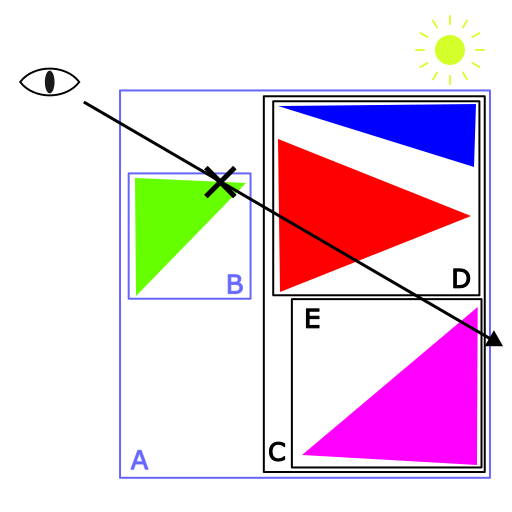
\includegraphics[width=.9\linewidth]{images/FirstHit.png}
        \caption{First-hit traversal.}
        \label{fig:traversal-first-hit}
    \end{subfigure}%
    \begin{subfigure}{.33\textwidth}
        \centering
        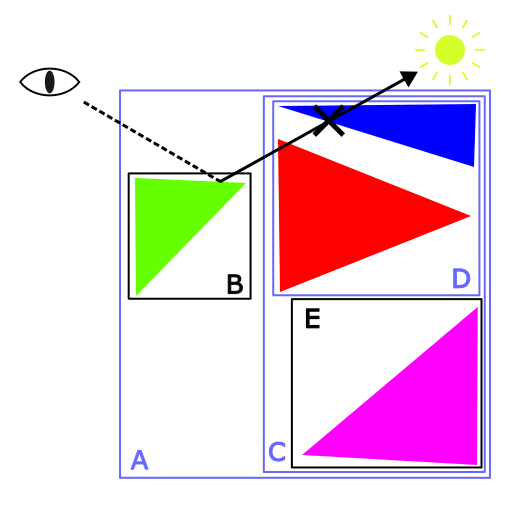
\includegraphics[width=.9\linewidth]{images/AnyHit.png}
        \caption{Any-hit traversal.}
        \label{fig:traversal-any-hit}
    \end{subfigure}%
    \begin{subfigure}{.33\textwidth}
        \centering
        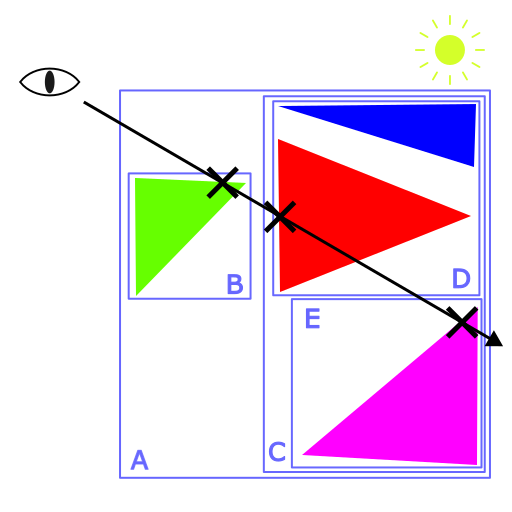
\includegraphics[width=.9\linewidth]{images/MultiHit.png}
        \caption{Multi-hit traversal.}
        \label{fig:traversal-multi-hit}
    \end{subfigure}
    \label{fig:traversal-hit-types}
    \caption{Hit traversal types demonstrated on a simple scene with triangles as primitives, bounding volumes, a camera, and a light source.}
\end{figure*}

The whole point of spatial acceleration data structures for ray tracing is to reduce the number of ray-primitive intersections at the cost of traversing the data structure. In this section the thesis describes the basic types of traversal.

\newpage
\paragraph{}There are three main types of traversal:
\begin{itemize}
    \item First-hit traversal (closest hit); finds the object nearest to the ray origin in the ray direction. The typical use case are primary and secondary rays in ray/path tracing. Figure \ref{fig:traversal-first-hit} shows this hit type.
    \item Any-hit traversal (occlusion test); finds any object in the ray direction starting from the ray origin. This is useful for shadow computation or ambient occlusion. Figure \ref{fig:traversal-any-hit} shows this hit type.
    \item Multi-hit traversal; finds all or \textit{h} closest intersections from the viewpoint. Used when dealing with non-refractive transparent surfaces, it avoids the need to retrace another ray from the root each time a ray hits an object. Figure \ref{fig:traversal-multi-hit} shows this hit type.
\end{itemize}

\paragraph{First-hit traversal} is most used for computing radiance at a shading point and most ray tracing engines are optimized for this kind of traversal. For binary BVHs it is straightforward to efficiently implement this just by pushing the farther child onto the stack and traversing the closer one first. When it comes to wide BVHs, there are $k!$ orders of traversal for branching factor $k$, and each ray may intersect any number of child nodes. Due to this, the child nodes must be ordered from front to back to be efficient. There are two common heuristics for sorting. One option is to simply use the sign of the ray direction and the split axes used during construction. The other option is to use the ray distance to the bounding volumes of the child nodes and sort according to it. When traversing wide BVHs, generally only 0 to 3 child nodes are intersecting, for any $k$, so it is possible to code a preset path to sort this small number of nodes and perform a complete sort only if there are 4 or more intersecting child nodes. \cite{Meister2021}

\paragraph{Any-hit traversal} or occlusion rays account for a large portion of the total rays used for ray tracing, for example when computing soft shadows from area lights, illumination from many lights or evaluating ambient occlusion. There is no need to visit all intersections front to back when calculating occlusion in a scene without any transparent geometry. Traversal can terminate the moment a ray intersects with any object. Any-hit traversal can have its own dedicated BVH with different metrics than first-hit traversal. \cite{Meister2021}

\paragraph{Multi-hit traversal} finds all intersections or $h$ nearest intersections inside a scene along a given ray. It is a generalization of first-hit traversal. Multi-hit traversal addresses the issues that first-hit traversal has with planar objects — self-intersection, particularly when handling two transparent materials next to each other (such as glass and water). Another use case is with reflected and refracted rays. When these rays are traced with a negative $\epsilon$-offset or a positive $\epsilon$-offset, the correct primitive intersections might be repeated or missed completely. There are two types of multi-hit traversal: those that find a limited number of intersections, where we can use a pre-allocated buffer to store the required intersections, and those that need to find all of them. When all intersections are required, it is usually not possible to predict their number. In this case, a method that works without dynamically allocating the list/buffer is preferred due to the overhead of reallocation. The same applies when a lot of intersections are needed. \cite{Meister2021}

\subsubsection{GPU traversal}

Traversal on GPUs is challenging because GPUs execute 32 threads in a parallel SIMD block called a \textit{warp}. This causes issues with non-locality of data access and control flow when using any acceleration data structure. To decrease the wait time of threads in a warp that have already completely traversed the given rays, new rays are loaded from a global work queue using \textit{persistent threads}. The traversal loop can be broken up into two independent loops to mitigate the control flow divergence.  The two loops are: iterating over the hierarchy and iterating over the primitives\cite{AL09}. To distribute the threads between these two loops, each on is implemented as either an \textit{if} block or a \textit{while} block. The So called \textit{if-if} traversal alternates the testing of nodes and primitives if \textbf{any} of those threads need to process an inner or a leaf node, respectively. On the other side in the \textit{while-while} traversal the hierarchy is traversed until all threads reach a leaf node, before all thread switch to iterating over primitives, This might lead to only a single thread being active in a warp, the switch to the other block is conditioned by a waiting thread count threshold instead of waiting for all of them. In addition, to increase the memory throughput at the cost of a few more traversed inner nodes, the traversal is continued, in the case of \textit{while-while} traversal, until a second leaf node is reached. The \textit{persistent speculative while-while} algorithm, which you can find in Algorithm \ref{alg:while-while}, shows the traversal algorithm with all discussed optimizations. \cite{Meister2021}

\definecolor{darkgreen}{RGB}{0,150,0}

\begin{algorithm}[h!tb]
\caption{Persistent speculative while-while traversal algorithm. Speculative traversal of inner nodes is marked in blue and ray fetching for persistent threads in green.\cite{Meister2021}}
\label{alg:while-while}
\begin{algorithmic}[1]
\State \textit{ray} = fetch\_ray()
\State \textit{node} = \textit{root}
{\color{blue}\State \textit{leaf} = $\varnothing$}
\While{{\color{darkgreen}\textit{ray} $\neq \varnothing$}}
    \State /* \textsc{Iteration over the hierarchy} */
    \While{\textit{node} does not contain primitives}
        \State traverse to the next \textit{node}
        \color{blue}
        \If{\textit{node} contains primitives \textbf{and} \textit{leaf} = $\varnothing$}
            \State \textit{leaf} = \textit{node}
            \State traverse to the next \textit{node}
        \EndIf
        \If{number of (\textit{leaf} $ \neq \varnothing$) per warp $>$ \textit{threshold}}
            \State break
        \EndIf
        \color{black}
    \EndWhile
    \State /* \textsc{Iteration over the primitives} */
    \While{\textit{leaf} or \textit{node} contain untested primitives}
        \State perform a ray-primitive intersection test
        \color{darkgreen}
        \If{\textit{ray} is terminated}
            \State \textit{ray} = fetch\_ray()
            \State \textit{node} = \textit{root}
        \color{black}
        \EndIf
    \EndWhile
\EndWhile
\end{algorithmic}
\end{algorithm}

The main performance limiter of GPU traversal is latency \cite{Guthe14} and not memory bandwidth or computation operation speed. There are more optimizations available. For example, loop unrolling can provide more instructions that the GPU is able to reorder, or having a wider BVH can help make individual instructions more independent. Sorting children using a predefined sorting network instead of a full sorting algorithm can also help to have more independent instructions. \cite{Meister2021}


% ----------------------------------------
\clearpage
\section{Parallel locally ordered clustering for BVHs}

The authors \cite{MB17} propose an algorithm using parallel locally-ordered clustering (PLOC) for BVH construction. The algorithm consists of two main ideas: First, locally-ordered clustering on a large number of clusters is performed in parallel. Second, to identify the nearest neighbors for clusters, Morton codes are used to sort and search the sorted sequence with local exploration instead of a complete nearest neighbor search.

Firstly, the thesis will describe these two ideas in more depth in the coming sections, and then it will provide a description of the original authors complete algorithm.

\subsection{Parallel locally ordered clustering}
\label{sec:ploc-aglomerative-clustering}

The starting point of the agglomerative clustering algorithm is a scene with primitives (triangles) forming $n$ clusters with a single primitive per cluster ($n$ being the number of primitives). These starting clusters are the leaves of the BVH. The algorithm then builds the higher levels by merging the clusters from the lower levels.

The distance function $d$ between two clusters $C_1$ and $C_2$ is defined as the surface area $A$ of an AABB that tightly encloses $C_1$ and $C_2$ \cite{WBKP08}:

\begin{equation}
    d(C_1, C_2) = A(\mathcal{B}(C_1 \cup C_2)) = A(\mathcal{B}(\cup(C_1, C_2))),
\end{equation}

where $\cup(C_1, C_2)$ is the clustering operator and $\mathcal{B}(C)$ is the AABB tightly enclosing cluster $C$. The function $d$ conforms to a non-decreasing property:

\begin{equation}
    d(C_1, C_2) \leq d(C_1 \cup C_3, C_2) : \forall C_1, C_2, C_3. 
\end{equation}

Walter et al. \cite{WBKP08} used the non-decreasing property and proposed the \textit{locally-ordered} agglomerative clustering algorithm. No better neighbor will emerge in the future if the nearest neighbors of two clusters \textit{mutually correspond} (both are each others nearest neighbors). The algorithm can then safely merge the mutually corresponding clusters together. This property is exploited in the following algorithm and is applied to all pairs of mutually corresponding clusters in parallel.

\subsection{Approximate nearest neighbor search}

\begin{figure*}[h!tb]
    \centering
    \begin{subfigure}{.5\textwidth}
        \centering
        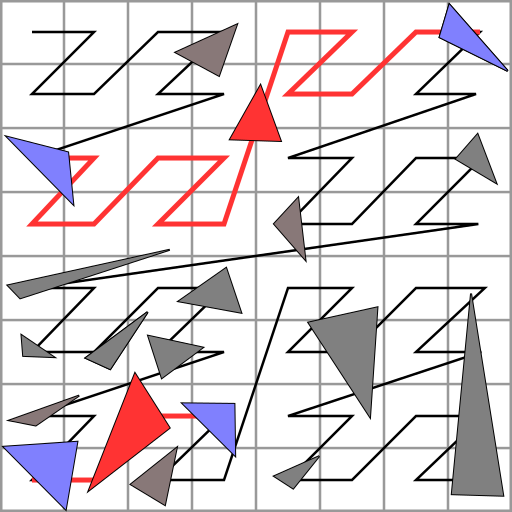
\includegraphics[width=.8\linewidth]{images/PLOC_nnsearch_r1.png}
    \end{subfigure}%
    \begin{subfigure}{.5\textwidth}
        \centering
        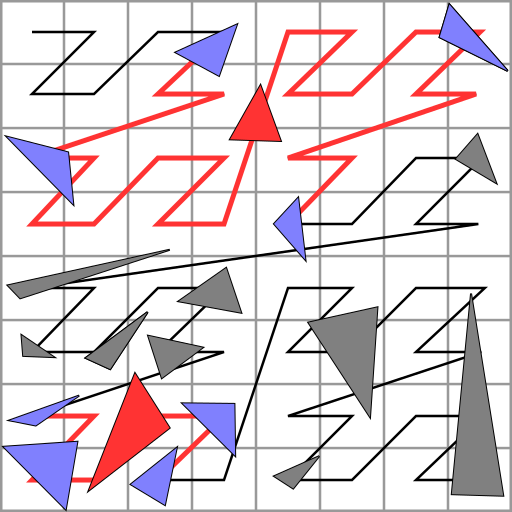
\includegraphics[width=.8\linewidth]{images/PLOC_nnsearch_r2.png}
    \end{subfigure}
    \caption{PLOC nearest neighbor search for $r = 1$ (left) and $r = 2$ (right). Clusters (red) search for their nearest neighbor (blue) along the Morton curve. \cite{MB17}}
    \label{fig:ploc-nn}
\end{figure*}

Each cluster needs to identify its nearest neighbors. Naïve evaluation would take $\mathcal{O}(n^2)$ time for $n$ clusters, which is inefficient and insufficient for large $n$.

The authors propose an alternative way to identify the nearest neighbors for all clusters. The clusters are sorted based on their centroids Morton codes. Then, for each nearest neighbor search, the algorithm just needs to use the 1D range search of the Morton curve to identify the nearest neighbor. To search for the nearest neighbors of cluster $C_i$ with index $i$, it searches the sorted sequence in the interval $\langle i-r,i+r \rangle$, where $r$ is the search radius. For every cluster $C_j, j \in \langle i-r,i+r \rangle \setminus {i}$, the algorithm evaluates the distance between the two clusters $d(C_i,C_j)$. The candidate $C_j$ with the smallest distance $d$ is selected as the nearest neighbor. An illustration can be seen in Figure \ref{fig:ploc-nn}. \cite{MB17}

Even though this method only finds the approximate nearest neighbors, it seems to be enough, as the actual nearest cluster pairs are found using the mutual cluster correspondence described in Section \ref{sec:ploc-aglomerative-clustering}. Authors \cite{MB17} claim that the approximate nearest neighbor search actually has a slightly positive influence on the BVH trace performance for some scenes due to the Morton codes providing implicit spatial subdivision corresponding with hierarchical spatial median splits. This stems from a better cluster separation for the top part of the BVH tree, resembling top-down methods and providing better correlation of the SAH cost and trace time \cite{AK13}. 

\subsection{Algorithm details}

\begin{figure}[h!tb]
    \centering
    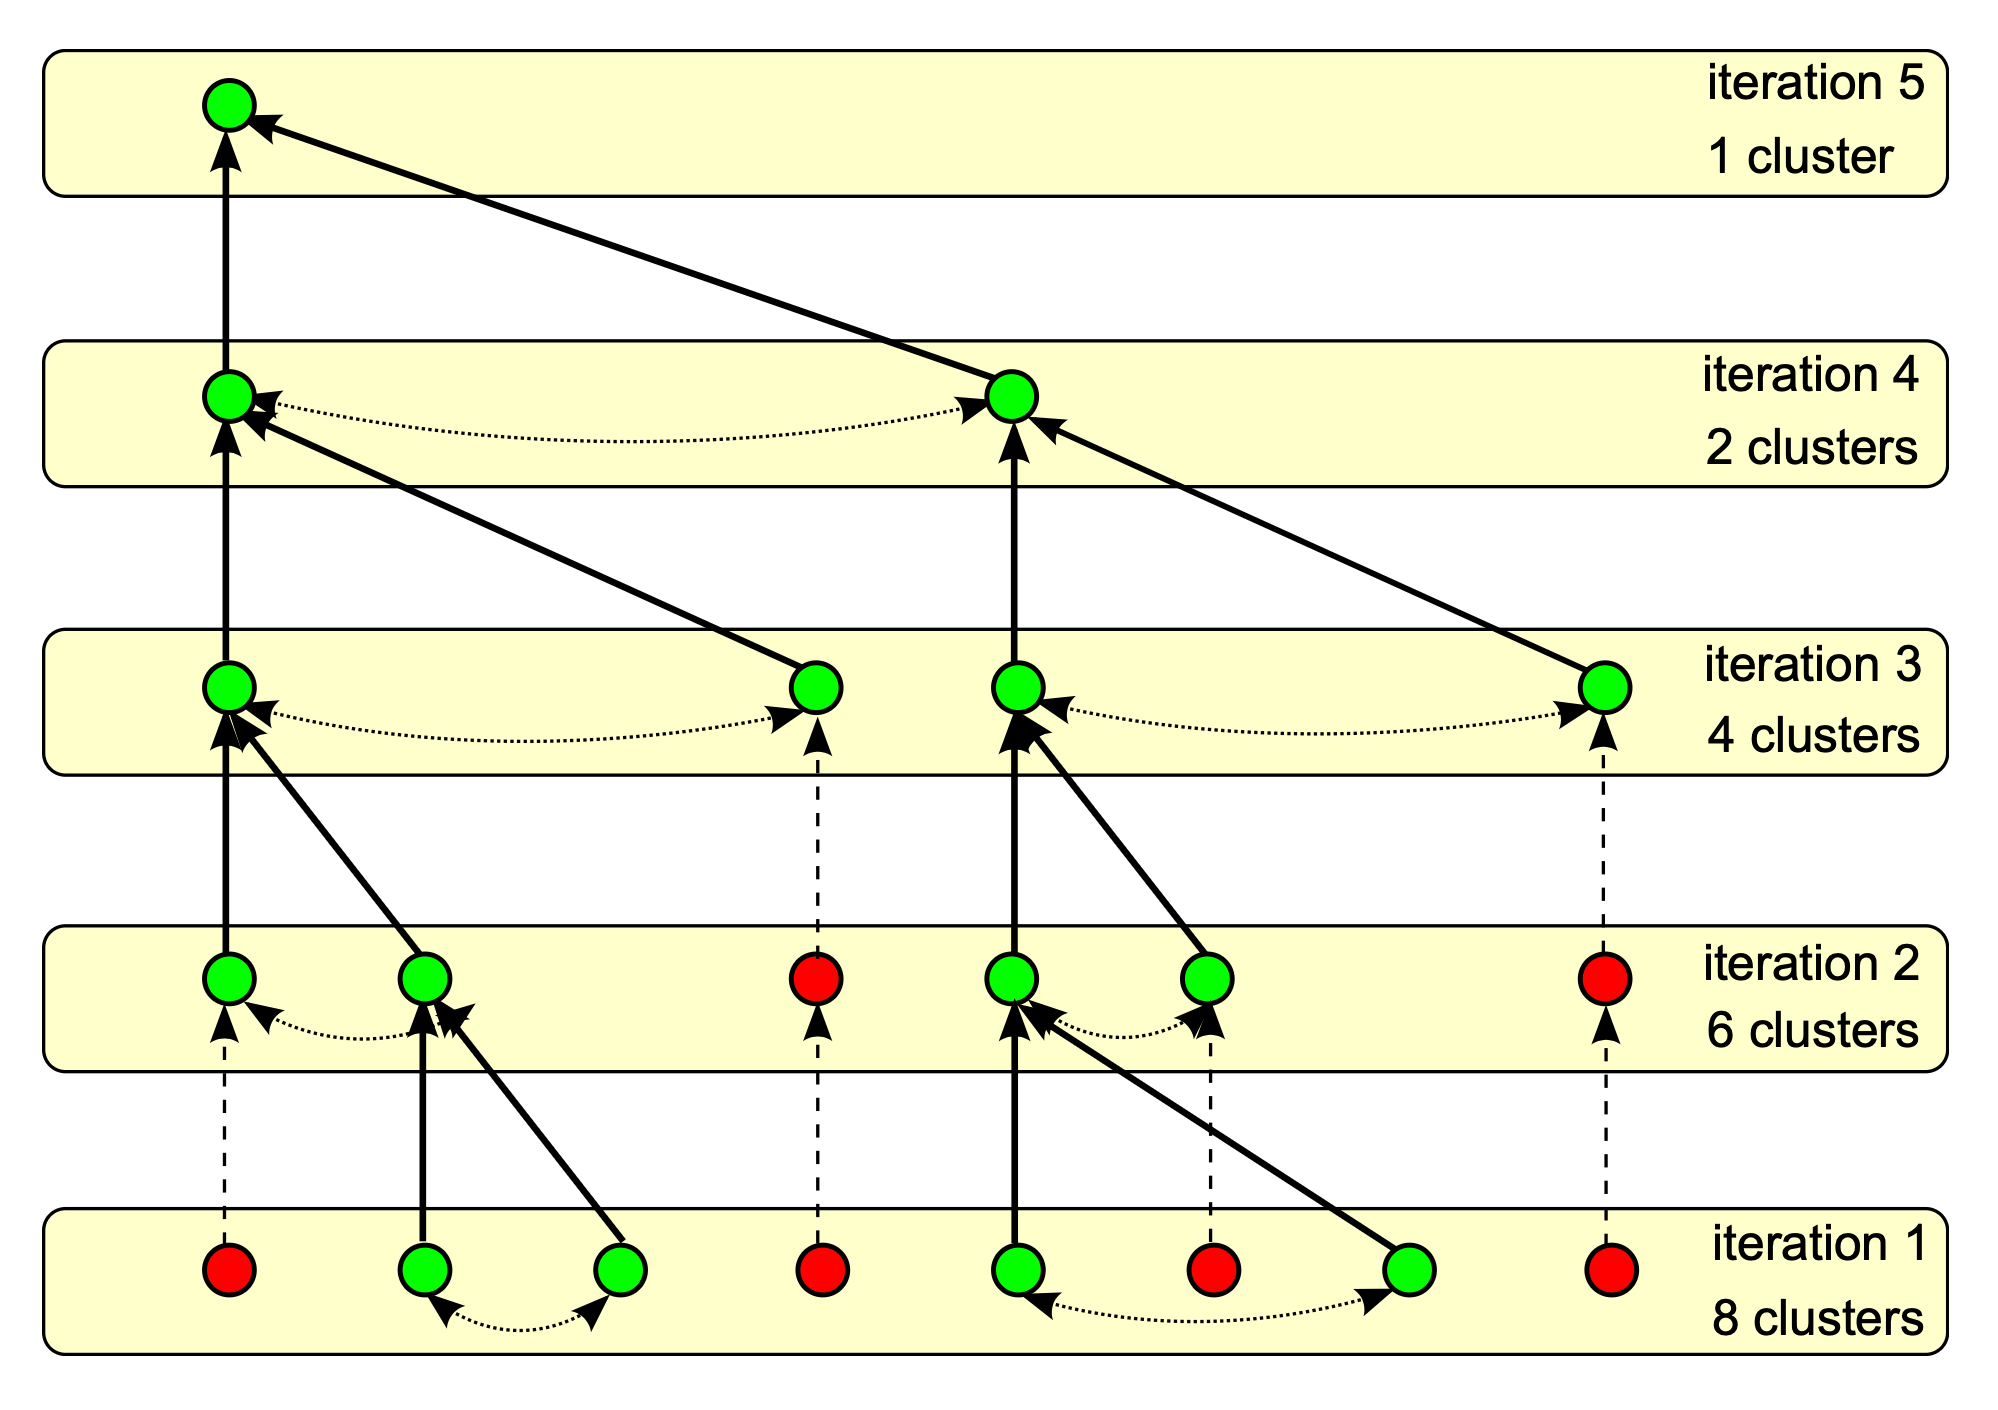
\includegraphics[width=0.8\linewidth]{images/PlocIterations.png}
    \caption{PLOC iterations. In each iteration, mutually corresponding clusters are merged (green nodes connected by dots). Newly merged clusters (green nodes deriving from two nodes from the previous iteration) and untouched clusters (red nodes) enter the next iteration. \cite{MB17}}
    \label{fig:ploc-iterations}
\end{figure}

\definecolor{nncolor}{RGB}{180,0,0}
\definecolor{mergecolor}{RGB}{0,180,0}
\definecolor{compactcolor}{RGB}{0,0,180}

Clusters are stored in two buffers (input and output), along with additional buffers to store the nodes of the resulting BVH, triangle indices, and several temporary buffers.

The algorithm starts by precomputing the bounding boxes and the Morton codes of scene primitives. It then sorts the primitives to order them along the Morton curve. Initially, all clusters are of size one, with one triangle in each.

The main loop starts and runs through a number of iterations. In each iteration, all nearest neighbor cluster pairs are merged. The main loop is made up of three phases: nearest neighbor search, merging, and compaction. After finishing each iteration, the input and output buffers are swapped. This repeats until there is only one cluster left. To guarantee that the main loop finishes and to solve the rare case of completely equidistant clusters, the algorithm prioritizes the nearest neighbor with the lower index. A depiction of several iterations of the algorithm can be seen in Figure \ref{fig:ploc-iterations}. \cite{MB17}

The pseudocode is shown in Algorithm \ref{alg:ploc}. The highlighted three main phases of the algorithm are:

\begin{itemize}
    \item The \textit{nearest neighbor search} phase (shown in {\color{nncolor} red}) searches for each cluster's nearest neighbor along the Morton curve in parallel using the 1D interval of clusters in the input buffer. Parameter $r$ denotes the interval, and it is clipped to prevent \textit{out-of-bounds} memory access. Each cluster keeps the nearest neighbor found (based on distance function $d$).
    \item The \textit{merging} phase (shown in {\color{mergecolor} green}) checks if each cluster is equal to its nearest neighbors nearest neighbor in parallel. If that is true, then both clusters are merged into one. To avoid conflict, the cluster with the lower index performs the merge. The first cluster (lower index) is replaced with the newly merged cluster, and the second cluster (higher index) is marked as invalid. At the same time, the algorithm creates a corresponding interior node for the new cluster. To determine the indices of the new interior nodes, a parallel prefix scan is performed on the new clusters. By adding the prefix scan value to the node counter, we can determine the actual node indices.
    \item The \textit{compaction} phase (shown in {\color{compactcolor} blue}) performs an exclusive parallel prefix scan to remove invalid clusters. The position of the node indices is determined by the prefix scan values and written to the output buffer. After some of the clusters have been merged and gaps appear in the Moron curve, a global prefix scan is needed to remove them. Note that the new clusters are not sorted again according to the Morton codes of their centroids. The authors observed that the clusters keep their ordering, which is sufficient enough for the nearest neighbor search algorithm, and so costly sorting can be avoided.
\end{itemize} 

\begin{algorithm}[h!tb]
\caption{PLOC algorithm pseudocode. The input of the algorithm is a sequence of $n$ clusters $C_0, C_1, \dots , C_{n-1}$ sorted along the Morton curve. Two auxiliary arrays are used: $\mathcal{N}$ (nearest neighbor indices) and $\mathcal{P}$ (exclusive prefix scan). The symbol $\emptyset$ denotes an invalid cluster. \cite{MB17}}
\label{alg:ploc}
\begin{algorithmic}[1]
    
\State $\mathcal{C}_{in} \gets \mathcal{C}_{out} \gets [C_0,\dots,C_{n-1}]$
\State $\mathcal{N} \gets \mathcal{P} \gets [0,\dots,n-1]$
\State $c \gets n$

\While{$c>1$}
    \For{$i \gets 0$ to $c-1$ \textbf{in parallel}}
        
        \color{nncolor}
        \State /* \textsc{Nearest Neighbor Search} */
        \State $d_{\min} \gets \infty$
        \For{$j \gets \max(i-r,0)$ to $\min(i+r,c-1)$}
            \If{$i \ne j \land d_{\min} > d(\mathcal{C}_{in}[i],\mathcal{C}_{in}[j])$}
                \State $d_{\min} \gets d(\mathcal{C}_{in}[i],\mathcal{C}_{in}[j])$
                \State $\mathcal{N}[i] \gets j$
            \EndIf
        \EndFor
        
        \color{black}
        \State $\textsc{Barrier}()$
        
        \color{mergecolor}
        \State /* \textsc{Merging} */
        \If{$\mathcal{N}[\mathcal{N}[i]] = i \land i < \mathcal{N}[i]$}
            \State $\mathcal{C}_{in}[i] \gets \textsc{Cluster}(\mathcal{C}_{in}[i],\mathcal{C}_{in}[\mathcal{N}[i]])$
            \State $\mathcal{C}_{in}[\mathcal{N}[i]] \gets %\color{black}\emptyset\color{compactcolor}$
            \emptyset$
        \EndIf
        
        \color{black}
        \State $\textsc{Barrier}()$
        
        \color{compactcolor}
        \State /* \textsc{Compaction} */
        \State $\mathcal{P}[i] \gets \textsc{PrefixScan}(\mathcal{C}_{in}[i] \ne %\color{black}\emptyset\color{compactcolor}$
        \emptyset)$
        %\If{$\mathcal{C}_{in}[i] \ne \color{black}\emptyset\color{compactcolor}$}
        \If{$\mathcal{C}_{in}[i] \ne \emptyset$}
            \State $\mathcal{C}_{out}[\mathcal{P}[i]] \gets \mathcal{C}_{in}[i]$
        \EndIf
        
        \color{black}
        \State $\textsc{Barrier}()$
        
    \EndFor
    
    \State $c \gets \mathcal{P}[c-1]$
    
    \If{$\mathcal{C}_{in}[c-1] \ne \emptyset$}
        \State $c \gets c+1$
    \EndIf
    
    \State $\textsc{Swap}(\mathcal{C}_{in},\mathcal{C}_{out})$
    
\EndWhile

\end{algorithmic}
\end{algorithm}


% ----------------------------------------
\clearpage
\section{Extended Morton codes for BVH construction}

Extended Morton codes \cite{Vinkler2017} propose to extend Morton codes, which are used for spatial sorting of scene primitives. These extensions increase the clustering and coherence from object sorting. They improve the primitive sorting especially well in non-uniformly distributed scenes. The proposed extensions enhance the basic Morton code by encoding object size, applying adaptive ordering of the individual bits, and using variable bit counts for different axes. Extended Morton codes lead to higher quality BVH, particularly for BVH build algorithms that heavily rely on spatial coherence of Morton code sorting. The method is easy to implement into algorithms that already use Morton codes and does not increase the build time significantly.

\subsection{Morton code based spatial sorting}

\subsubsection{Morton codes}

Morton code is a space filling curve that provides relatively coherent ordering of quantized vectors, meaning that continuous Morton code sequences are spatially close together. Morton code maps quantized n-dimensional vectors into integer scalar values - codes. The resulting curve of consecutive codes is also known as the Z-curve because of its shape when used with 2D data (see Figure \ref{fig:morton-space-filling}). Many more space filling curves exist and some with even more coherent spatial ordering \cite{Samet2006}, but Morton code became popular due to its simplicity and cheap computation time using only bit interleaving operations.

The Morton code is made up of a set number of bits that serves as its major parameter, along with the number of dimensions. An \(n\) bit Morton code of a three dimensional vector $v = (v_x, v_y, v_z) \in \langle 0, 1 \rangle^3$ is computed by first quantizing the coordinates $v^* = \{ v^*_x, v^*_y, v^*_z \} \in \langle 0,2^{n/3} \rangle \times \langle 0,2^{n/3} \rangle \times \langle 0,2^{n/3} \rangle$ and then the code is then constructed by interleaving bits of the components of $v^*$ \cite{Vinkler2017}. 

The bit interleaving operation can be performed using multiplication and sums as first conceived \cite{Morton1966}. Alternatively, precomputed lookup tables can be used for certain bit ranges and then combined by additions and shifts.

\begin{figure}[h!tb]
\centering
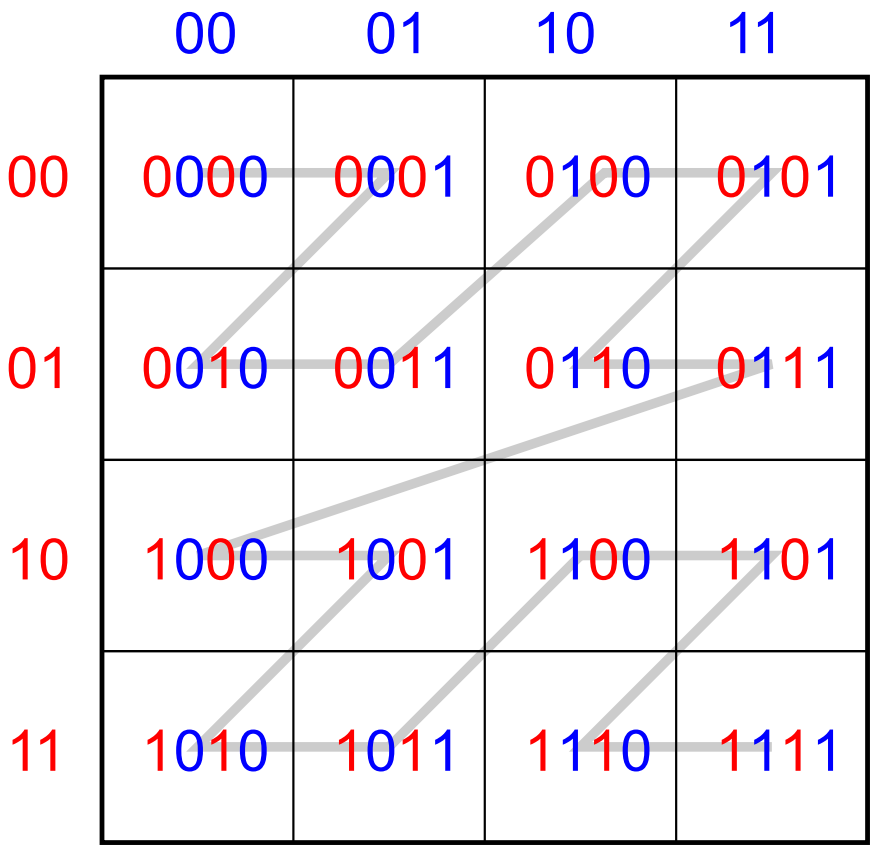
\includegraphics[width=0.8\textwidth]{images/MortonCodeSpaceFilling.png}
\caption{Space-filling curve representation of Morton codes in 2D space 
\cite{Vinkler2017}.}
\label{fig:morton-space-filling}
\end{figure}

\subsubsection{Constructing BVH using Morton codes}

Since Morton codes encode the spatial location of positions in 3D space, they can be easily used for the construction of spatial data structures. Scene primitives are represented as points and sorted according to their individual Morton codes, by doing this multi-scale clusters of primitives can form. Boundaries between clusters are defined by changes in bit positions. \cite{Vinkler2017}

This property is exploited by spatial data structures that use Morton codes. For example, the LBVH method \cite{Lauterbach2009} sorts primitives according to the Morton codes of their centroids. Starting from the most significant bit, the BVH tree is formed by splitting the current node (starting from the root with all primitives) in two according to the value of the bit in the centroid of the primitive at that position. Thus, the BVH topology is solely given by the computed Morton codes.

\subsection{Extended Morton codes}

This section summarizes the individual extensions proposed to the standard Morton Codes. These extensions modify the encoded data, their ordering, and the number of bits dedicated to each axis (or other encoded data).

\subsubsection{Encoding object size}

Real-world scenes typically contain geometric primitives with widely varying sizes. When primitives are sorted only by their centroid positions, spatial clustering can become inefficient. Although centroids may be spatially close, the resulting common bounding volume may be poorly fitted, particularly affecting smaller objects in the cluster. Large primitives propagate their larger bounding volumes not just at individual leaf nodes, but along the entire path from leaf to root, degrading overall BVH quality. Therefore, it is better to isolate such large objects and potentially position them at higher tree levels to minimize their influence on the remaining hierarchy. \cite{Vinkler2017}

The authors propose encoding the primitive size directly into the Morton code by injecting additional bits representing the diagonal length of the object. In the simplest configuration, the size information uses the same bit allocation as the three spatial axes, resulting in a 4-dimensional Morton code constructed by interleaving quantized coordinates $(x, y, z, s)$, where $s$ represents the primitive size normalized to the scene bounding box diagonal. With regular bit interleaving pattern (e.g., $xyzsxyzs...$), the resulting code structure mirrors octree-like subdivision, where each triple of spatial splits subdivides volumes into eight equal sub-volumes with half the original diagonal size. The size bits can then directly determine whether an object is larger or smaller than the current volume primitives. If the size bit is set to 1, the bounding box exceeds the dimensions of the current box and is separated into a distinct subtree, as can be seen in Figure~\ref{fig:morton-construction}. The authors also experimented with encoding the surface area instead of the diagonal length, but the diagonal length produced slightly better overall performance in their evaluation \cite{Vinkler2017}.

\begin{figure}[h!tb]
\centering
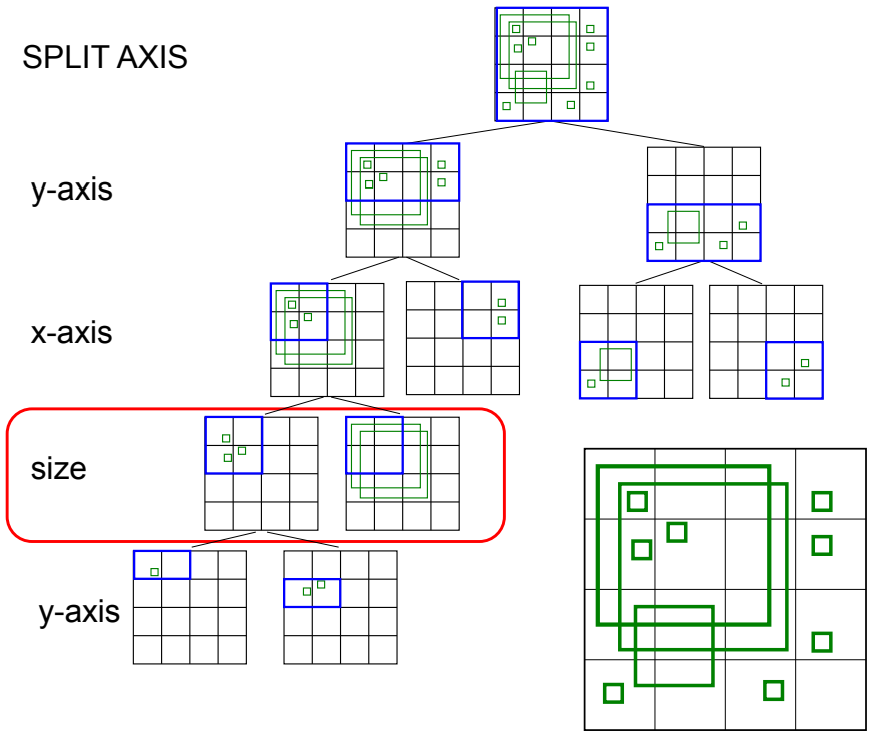
\includegraphics[width=0.8\textwidth]{images/MortonCodeConstruction.png}
\caption{Visual representation of Morton code construction in 3D space 
\cite{Vinkler2017}. Size bit is used to subdivide objects in the third level.}
\label{fig:morton-construction}
\end{figure}

\paragraph{Using fewer size bits} is beneficial in certain scenarios, particularly with shorter bit codes (32-bit Morton codes) or large scenes with many millions of primitives. Encoding object size in a coarser manner can be enough to preserve the primary subdivision potential of spatial positions. The authors propose reducing size bit allocation by injecting size bits only every 7th bit position - after two complete cycles of splits along each spatial axis - while maintaining the ability to separate small and large objects at appropriate tree levels. \cite{Vinkler2017}

\subsubsection{Adaptive axis order}

The authors discovered through experimentation that the ordering of spatial axis bits within the Morton code significantly influences BVH quality. Specifically, arranging axes in descending order by scene extent - placing the largest dimension first - consistently improved results, as splitting along larger axes first produces centroid clusters that are more cuboid-shaped and spatially compact compared to fixed $(xyz)$ ordering. \cite{Vinkler2017}

\subsubsection{Variable bit count}

The adaptive axis ordering concept can be generalized further by allowing variable bit allocation across different axes, which is particularly beneficial for scenes with non-uniform extents in individual axes, such as terrain or city models that extend primarily along two dimensions. The authors propose a major-axis-based method, where the largest axis is selected for each bit position, and the bounding box is halved along that axis before the next bit selection. Injection of optional size bits is made at regular intervals (every 4th or 7th bit). Once all bits are assigned, the bit counts per-axis determine the appropriate quantization scales. \cite{Vinkler2017}

\subsubsection{Extension combinations}

Two versions are suggested by the original article. The pseudocode for version~1: the 64-bit EMC generation using adaptive axis order and size bits injected every 4th bit can be seen in Algorithm~\ref{alg:emc64var1}.The pseudocode for version~2: the 64-bit EMC generation using variable bit order, adaptive axis order, and size bits injected every 7th bit can be seen in Algorithm~\ref{alg:emc64var2}. The \textsc{Expand} function inserts a variable number of zeroes before each bit of the input number. Notation: $X \ll Y$ corresponds to the left shift bitwise operation of integer $X$ by $Y$ bits, $\mid$ corresponds to the bitwise binary operation OR, and $\&$ corresponds to the bitwise binary operation AND. \cite{Vinkler2017}

% EMC Variant 1
\begin{algorithm}[H]
\caption{Pseudocode of the 64-bit EMC variant 2 generation. \cite{Vinkler2017}}
\label{alg:emc64var1}
\begin{algorithmic}[1]

\Function{Init}{$scene$}
  \State $a_0 = x,\; a_1 = y,\; a_2 = z,\; a_3 = size$
  \State \Call{sort}{$a_0..a_2$} \Comment{descending axis order using scene dimensions}
  \Comment{compute quantization scales}
  \State $s_0 = 2^{16} / scene.box.size[a_0]$
  \State $s_1 = 2^{16} / scene.box.size[a_1]$
  \State $s_2 = 2^{16} / scene.box.size[a_2]$
  \State $s_3 = 2^{16} / scene.diagonal.length$
\EndFunction

\Function{Expand}{$X$}
  \State $v = 0,\; mask = 1$
  \For{$i = 0$ to $15$ step $1$}
    \State $v = v \mid ((X \& mask) \ll (3 \cdot  i))$
    \State $mask = mask \ll 1$
  \EndFor
  \State \Return $v$
\EndFunction

\Function{Code}{$triangle$}
  \State $v = triangle.box.center-scene.box.min$
  \State $size = triangle.box.diagonal.length$
  \State $v^*_0 = s_0 \cdot v[a_0]$
  \State $v^*_1 = s_1 \cdot v[a_1]$
  \State $v^*_2 = s_2 \cdot v[a_2]$
  \State $v^*_3 = s_3 \cdot size$
  \State \Return 
    $(\Call{Expand}{v^*_0} \ll~3) \;\mid\; 
      (\Call{Expand}{v^*_1} \ll 2) \;\mid\; 
      (\Call{Expand}{v^*_2} \ll 1) \;\mid\; 
      \Call{Expand}{v^*_3}$
\EndFunction

\end{algorithmic}
\end{algorithm}


\begin{algorithm}[h!tb]
\caption{Pseudocode of the 64-bit EMC variant 2 generation. \cite{Vinkler2017}}
\label{alg:emc64var2}
\begin{algorithmic}[1]

\Function{Init}{$scene$}
  \For{$i = 0$ to $63$}
    \If{$i$ is the 7th bit}
      \State $axes[i] = 3$ \Comment{insert size bit}
    \Else
      \State $axes[i] = scene.box.size.maxAxis$ \Comment{pick the largest axis}
      \State $scene.box.size.maxAxis /= 2$ \Comment{halve the largest axis}
    \EndIf
  \EndFor
  \State $bits_{0..3} = axes.sum(0..3)$ \Comment{number of bits in each axis}
  \State $shifts_{0..3} = axes.shifts(0..3)$ \Comment{shifts between bits in each axis}
  \Comment{compute quantization scales}
  \State $s_0 = 2^{bits_0} / scene.box.size[a_0]$
  \State $s_1 = 2^{bits_1} / scene.box.size[a_1]$
  \State $s_2 = 2^{bits_2} / scene.box.size[a_2]$
  \State $s_3 = 2^{bits_3} / scene.box.diagonal.length$
\EndFunction

\Function{Expand}{$axis,\; X$}
  \State $v = 0,\; mask = 1$
  \For{$i = 0$ to $bits_{axis}-1$}
    \State $v = v \mid ((X\ \&\ mask) \ll (shifts_{axis}[i]))$
    \State $mask = mask \ll 1$
  \EndFor
  \State \Return $v$
\EndFunction

\Function{Code}{$triangle$}
  \State $v = triangle.box.center - scene.box.min$
  \State $size = triangle.box.diagonal.length$
  \State $v^*_0 = s_0 \cdot v[a_0]$
  \State $v^*_1 = s_1 \cdot v[a_1]$
  \State $v^*_2 = s_2 \cdot v[a_2]$
  \State $v^*_3 = s_3 \cdot size$
  \State \Return
    $(\Call{Expand}{a_0, v^*_0}  \ll 3) \;\mid\;
      (\Call{Expand}{a_1, v^*_1} \ll 2) \;\mid\;
      (\Call{Expand}{a_2, v^*_2} \ll 1) \;\mid\;
      \Call{Expand}{a_3, v^*_3}$
\EndFunction
  
\end{algorithmic}
\end{algorithm}


% ----------------------------------------
\clearpage
\section{Skewed oriented bounding boxes}
\label{sec:sobb}

In the context of ray tracing, vast majority of BVH axis aligned bounding boxes (AABB) are used as the bounding primitives. Recently, tighter bounding volumes such as oriented bounding boxes (OBB) \cite{OR85} or discrete orientation polytopes (DOP) \cite{KZ97} have been discovered to improve the performance of ray tracing at the cost of increasing the BVH constriction time \cite{KB24}.

In the this section of the thesis, the Skewed oriented bounding boxes (SOBB) \cite{KB25} are introduced as a generalization of the oriented bounding box with the skew transformation. The resulting bounding primitive corresponds to a parallelepiped defined by three slabs. In the following sections, you can read about the geometry, surface area calculations, ray intersection, and BVH application of the SOBB.

\subsection{Definition of SOBB}

This section explains the SOBB as a shape. Firstly its geometric definition and then how to compute its surface area -- an essential operation for tightly fitting the primitives and clusters of primitives during BVH construction.

\subsubsection{Geometry of SOBB}

Skewed oriented bounding box is a bounding volume for a set of scene primitives, its geometrical representation corresponds to a \textit{parallelepiped}. A parallelepiped is an object comprised of three pairs of parallel faces, each being a parallelogram. Well known 3D objects, such as a cube or a rectangular cuboid, are general parallelepipeds with a set of edge and angle constraints. Cuboid shapes are especially important as bounding volumes for entities in computer graphics, either as AABBs or OBBs. \cite{KB25}

Multiple representations can be used to describe a parallelepiped: (1) The \textit{edge-based representation} consists of three edge vectors. These vectors are a basis for a vector space with parallelepiped edges with unit lengths aligned with the axes. (2) The \textit{slab-based representation} forms the parallelepiped as an intersection of three slabs, each comprised of two parallel planes defined by a normal vector and distances from origin. Both representations are illustrated in Figure \ref{fig:sobb-geometry}. For different computational tasks, one representation may be more beneficial than the other. \cite{KB25}

It is beneficial to maintain a single representation throughout the entire pipeline for efficiency. Slab representation is often favored because of the efficient ray-object intersection. \cite{KB25}

\begin{figure}[h!tb]
    \centering
    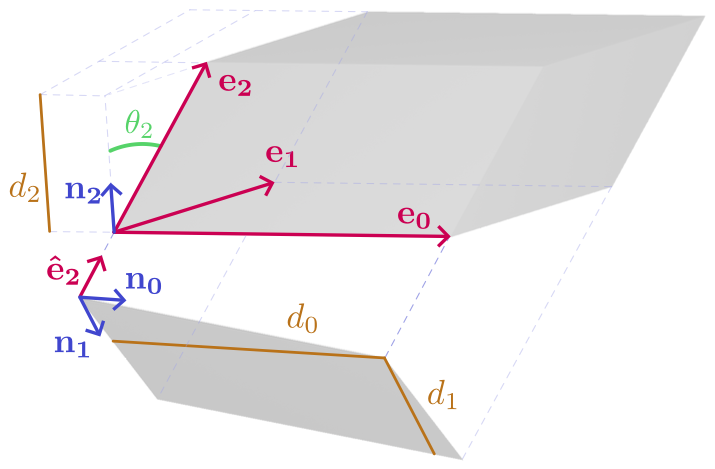
\includegraphics[width=0.8\linewidth]{images/SOBB_geometry.png}
    \caption{Parallelepiped with edges $e_0$, $e_1$ and $e_2$. Slab representation with slab normals $n_0$, $n_1$ and $n_2$ combined with their respective widths $d_0$, $d_1$ and $d_2$ \cite{KB25}.}
    \label{fig:sobb-geometry}
\end{figure}

\subsubsection{Surface area of SOBB}

Surface area is on the other hand (unlike ray-object intersection) more easily formulated in the edge representation. The surface area formula for a parallelepiped with edges $e_0$, $e_1$ and $e_2$ (as shown in Figure \ref{fig:sobb-geometry}) is formed by summing the area of the face parallelograms \cite{KB25}:
\begin{align}
    A_{pp}(\mathbf{e}_0, \mathbf{e}_1, \mathbf{e}_2)
        &= 2 \big( A_{pg}^0(\mathbf{e}_0, \mathbf{e}_1)
        + A_{pg}^1(\mathbf{e}_1, \mathbf{e}_2)
        + A_{pg}^2(\mathbf{e}_2, \mathbf{e}_0) \big) \notag \\
        &= 2 \big( \lvert \mathbf{e}_0 \times \mathbf{e}_1 \rvert
        + \lvert \mathbf{e}_1 \times \mathbf{e}_2 \rvert
        + \lvert \mathbf{e}_2 \times \mathbf{e}_0 \rvert \big)
    \label{eq:sobb-edge-surface-area}
\end{align}

To compute each parallelogram's surface area, the following formula can be used \cite{KB25}:
\begin{equation}
    A_{Pg}^{0}(\mathbf{e}_{0}, \mathbf{e}_{1}) = \lvert \mathbf{e}_{0} \times \mathbf{e}_{1} \rvert = \lvert \mathbf{e}_{0} \rvert \lvert \mathbf{e}_{1} \rvert \sin \alpha_{0} = \lvert \mathbf{e}_{0} \rvert \lvert \mathbf{e}_{1} \rvert \lvert \hat{\mathbf{e}}_{0} \times \hat{\mathbf{e}}_{1} \rvert
    \label{eq:pg-edge-surface-area}
\end{equation}
or transformed to the slab notation and simplified using the scalar triple product\cite{KB25}:
\begin{equation}
    A_{pg}^{0}(\mathbf{n}_{0}, \mathbf{n}_{1}, \mathbf{n}_{2}, d_{0}, d_{1}) = \ldots = \frac{d_{0} d_{1}}{\left| \det \big[ \mathbf{n}_{0} \ \mathbf{n}_{1} \ \mathbf{n}_{2} \big] \right|}
    \label{eq:pg-slab-surface-area}
\end{equation}

Surface area computation is especially important for BVH construction, so to avoid transitioning between slab and edge representations, the authors derived a formula for surface area computation for the slab representation \cite{KB25}:
\begin{equation}
    A_{pp}(n_0, n_1, n_2, d_0, d_1, d_2)
    = 2 \left( \frac{d_0 d_1 + d_1 d_2 + d_2 d_0}{\left|\det\left[\,n_0 \quad n_1 \quad n_2\,\right]\right|} \right)
    \label{eq:sobb-slab-surface-area}
\end{equation}

Equation \ref{eq:sobb-slab-surface-area} indicates that the surface area of a parallelepiped is inversely related to both the absolute value of the determinant of the matrix formed from the normal vectors of the slab and the volume of the unit parallelepiped generated by the normals of the slabs that determine the original parallelepiped. This volume (the value of the determinant) can serve as an indicator of orthogonality of the basis of the parallelepiped. \cite{KB25}

\subsection{Construction and traversal of SOBB BVH}

This section reveals the algorithm for building SOBB and SOBB BVH. It also talks about the traversal of such BVH and about the associated memory consumption and layouts.

\subsubsection{SOBB construction using $k$-DOPs}

Each processed set of primitives is fitted with a high degree $k$-DOP, which is then sampled for a triplet of slabs. These three chosen slabs form the newly created SOBB and are stored in the final hierarchy. \cite{KB25}

As hinted earlier, a $k$-DOP consists of $k$ parallel planes defined by $k/2$ pairs of collinear but opposing normals. The candidate SOBB set is based on the discrete set of $k$-DOP normals, consisting of all combinations of three normals. Generally, a uniform distribution of normals should be aimed for. However, it may be practical to ensure that certain normal directions are available, such as those of an orthogonal AABB basis. The discrete sets of normals are obtained by the relaxation of random samples on the surface of a unit hemisphere. The size of the candidate set increases with the rate of $(k/2)^3$ (assuming that all normals are linearly independent). This has the effect that, even though higher $k$ values are likely to create better fitting SOBB, the space of candidates grows rapidly outside of computable feasibility. \cite{KB25}

The surface area of the SOBB is used to choose the best fitting SOBB. Candidate SOBBs are generated using the intermediate $k$-DOP representation and one of the following strategies:

\paragraph{$O(k^3)$ strategy.} Brute force can be used to find the optimal SOBB for the given $k$-DOP by iterating over all SOBBs generated by the $k$-DOP triples, evaluating Equation \ref{eq:sobb-slab-surface-area} for each triplet. Then the triplet with the smallest surface area is chosen. The construction performance is significantly affected by the three nested loops, but provides the best possible BVH for given $k$-DOP. \cite{KB25}

\paragraph{$O(k^2)$ strategy.} To speed up construction, it is possible to make a trade-off: A basis vector is preselected, and then all available normal pairs are evaluated for surface area using Equation \ref{eq:sobb-slab-surface-area}. Since the goal is to minimize the total area, the normal with the narrowest slab present in the $k$-DOP is selected as the first axis. \cite{KB25}

\paragraph{$O(k)$ strategy.} If the previous strategy is still too expensive (for high $k$ values) an even faster heuristic can be used. The three vectors are picked one by one, using the limited information for each step. The first axis is chosen in the same way as in the $O(k)^2$ strategy, by choosing the normal with the narrowest slab. The second axis is chosen in a way to minimize the area of the resulting parallelogram formed by the two normals. It can be computed with the inverted Equation \ref{eq:pg-edge-surface-area}, so while working in the slab representation: $A_{pg} = d_0d_1 / sin\theta$, with $d$ being the slab width and $\theta$ the angle between the tested normals. As the first normal has already been set at this time, the equation can be simplified to $A_{pg} = d^2 / (1 - (n_0 \cdot n_1)^2)$. The final surface area of the SOBB face will be scaled proportionally using the last axis of the basis, which is unknown at this point. To select the last vector and form the final SOBB, we again iterate through the available normals and choose the one that minimizes the surface area generated by the triplet. \cite{KB25}

\subsection{SOBB BVH construction}

The construction is based on an existing AABB hierarchy, which is transformed into an SOBB hierarchy in a single bottom-up pass. The correctness of the bottom-up pass is guaranteed by using atomic operations and the fact that all child nodes are always processed before their parent. \cite{KB25}

The main task is to transform the AABB bounding volume into an SOBB bounding volume for each node. 

The transformation algorithm works like this. For each leaf node, a $k$-DOP is fitted to the geometry stored in the node by projecting the geometry on the $k$-DOP normals. Then the space of possible SOBBs generated by the $k$-DOP fitting is explored, and the best candidate is chosen to create the final SOBB of the leaf. For internal nodes, the bottom-up traversal continues by applying almost the same process, except to construct the node's $k$-DOP the algorithm merges the children $k$-DOPs instead of fitting all included geometries. \cite{KB25}

\subsubsection{Memory layout and intersection test}

The SOBB representation right after construction comprises the triples normals, each associated with a minimal and maximal projection. This totals $15$ floating-point values, which can be stored in multiple ways. Each storage strategy directly impacts the intersection test performed during traversal. \cite{KB25}

\paragraph{Direct slab normals layout.} Each slab is represented as four floating-point values by scaling the normal and storing the factor \cite{KB25}:
\begin{equation}
    \rho = \frac{1}{\max(p_{\max} - p_{\min}, \epsilon)}, \quad
    \mathbf{s} = \rho \cdot \begin{bmatrix} n_x & n_y & n_z & p_{\min} \end{bmatrix}^{T}
    \label{eq:sobb-direct-slab-layout}
\end{equation}

The intersection test then uses the standard branchless slab-based ray clipping test, with decoded slab values using the computed scaling. The SOBB with its three basis vectors can be stored using $12$ floating-point values, $48$ bytes per volume (in single precision). \cite{KB25}

\paragraph{Transformation matrix layout.} A bijective linear transformation from one parallelepiped to another can be found (assuming non-degenerate volumes). From this transformation it is possible to find a linear transformation of the SOBB to a unifrom $[-0.5, 0.5]^3$ AABB. The representation then stores the inverse of the affine transformation matrix as a $3 \times 4$ matrix representation of the SOBB. During traversal the transformation matrix is utilized to transform the given ray and perform the intersection test in the space of the unit AABB \cite{SVCNM21}. Like the slab normals, one bounding volume requires $48$ bytes of memory (again in single precision). \cite{KB25}

\paragraph{Indirect slab normals layout.} This representation saves significantly on used memory by not storing the three normals per SOBB explicitly, but instead storing only an index into a shared buffer of precomputed normals. Each slab is then represented only by its minimum and maximum projection values together with the corresponding normal index.

The normal indices require only a small number of bits (depending on $k$), resulting in $24$ bytes for storing the single-precision slab spans, with an additional $2$ bytes used to store the three normal indices. For example, for ($k = 64$), each index requires $5$ bits, i.e., 15 bits in total, which can be compactly stored in 2 bytes.

During ray--SOBB intersection, the corresponding normals must be fetched from the shared buffer. After this indirection, the standard branchless slab-based ray clipping test can be used without any further modifications.



% Measurement methodology
%---------------------------------------------------------------
\chapter{Acceleration data structure comparison and measurement}
\label{chap:measurement}
%---------------------------------------------------------------

\begin{chapterabstract}
This chapter explains the currently used methodology to measure and compare acceleration data structures, specifically bounding volume hierarchies. The measurement and testing done inside of this thesis, that you can find in later chapters, is based on the methodology explained in this chapter. 
\end{chapterabstract}

\section{Cost model for wide BVHs}

As explained in Section \ref{sec:cost-function}, cost models and functions are used to estimate the quality of a particular BVH. The quality is in terms of the expected number of operations needed to find the nearest ray-triangle intersection. The surface area heuristic \cite{GS87} is used the most. To remind the reader, here is the formula for the cost function:
\begin{equation}
    c(N) =
    \begin{cases}
        c_T + \displaystyle\sum_{N_c} \dfrac{SA(N_c)}{SA(N)}\,c(N_c) & \text{if } N \text{ is an interior node}, \\[6pt]
        c_I \lvert N \rvert & \text{otherwise},
    \end{cases}
    \label{eq:SAH-cost-model}
\end{equation}
where $c(N)$ is the cost of a subtree with root $N$, $N_c$ is a child node of $N$, $SA(N)$ is the surface area of the bounding volume of node $N$, and $|N|$ is the number of primitives on node $N$. To simplify the cost of traversal and intersection, constants $c_T$ and $c_I$ are used, respectively.

The recurrence is removed by unrolling:
\begin{equation}
    c(N) = \frac{1}{SA(N)} \left[ c_T \sum_{N_i} SA(N_i) + c_I \sum_{N_l} SA(N_l) \lvert N_l \rvert \right], 
    \label{eq:SAH-cost-model-unrolled}
\end{equation}
where $N_i$ are the interior nodes and $N_l$ are the leaf nodes.

However, this model is far from reality, as it does not take into account other factors such as the ray distribution, occlusions, the used rendering algorithm of the underlying hardware architecture. Nevertheless, most construction algorithms nowadays use this cost model to maximize the ray performance. Some construction algorithms exploit the fact that if only one primitive per leaf is used, then the cost function reduces simply to the sum of the surface areas of the bounding volumes in interior nodes. \cite{MB22}

The standard surface area heuristic does not take into account SIMD units, which most modern hardware architectures are equipped with, that allow multiple intersection tests to be processed at once. This is used for example in wide BVHs, where multiple bounding volumes at once can be tested against a single ray. Primitives in leaves are processed in a similar fashion, so it is advantageous to align the number of primitives per leaf with the SIMD width. To take into account this fact, a modified version of the cost model was created \cite{WBB08}:
\begin{equation}
    \label{eq:SAH-cost-model-SIMD}
    c(N) = \frac{1}{SA(N)}
    \left[
        c_T \sum_{N_i} SA(N_i)
        + c_I \sum_{N_l} SA(N_l)\, k \left\lceil \frac{|N_l|}{k} \right\rceil
    \right],
\end{equation}
where $k$ the SIMD width or the branching factor. This modified version of the cost model punishes leaves if their size is not aligned with $k$. $c_T$ is made independent of $k$ by multiplying the term by $k$. \cite{MB22}

\section{Construction time}

% Toto jsem si vymyslel sám, přesunout jinam?

The time required to construct the BVH is also important. That is especially true for real time ray/path tracing, where the frame budget is critically low. Construction time may be distributed among multiple frames if the complete reconstruction is not frequent, for example in static scenes, or the BVH can be adjusted when there are only small deformations to the scene. Of course, that is almost impossible for highly dynamic scenes, where the BVH is rebuilt on every frame. Build times are most commonly measured in milliseconds.

\section{Trace performance}

% Toto jsem si vymyslel sám, přesunout jinam?

To make trace performance measurement better for comparison, rays per second ($Mray/s$) are more easily compared between algorithms. Pure time to render a scene is not as explainable and hides details. Rays per second for each ray type provide a more detailed description. representation of the work distribution. This is a standard method for measuring trace performance \cite{MB22}. The types include primary rays (only a small number), secondary rays (most divergent), and occlusion/shadow rays (most abundant). 

\section{Cost and trace performance corelation}

There is a discrepancy between the BVH cost and the actual trace performance \cite{AK13}. The cost reduction of a BVH tree does not guaranty an improvement in trace performance. Top-down builders, such as the ones using SAH for local improvement during construction, provide locally well optimized top levels, which gives good results, because almost all rays visit them, even though they have a higher cost than other approaches. To measure this fact, a ratio between trace time and cost is computed, which expresses the time needed for a unit cost. This value can be considered as a correction to the actual cost values. The corrected cost, which actually corresponds to the trace times, can be obtained by multiplying the cost by these values. \cite{MB22}

%- BVH
%   - DFS/BFS order
%   - node size/layout
%   - AoS/SoA data layout
%   - same traversal algorithm
%   - Morton code bit length
%   - search radius
%   - same width of wide BVH / SIMD
%- the same raytracing/pathtracing algorithm
%   - samples per pixel
%   - resolution
%   - maximum recursion depth
%- diverse scenes
%   - architecture/object, flat/terrain, inside/outisde
%   - increasing complexity (# of triangles, shapes of triangles)
%- hardware
%- cost model evaluation
%   - advaced model with SIMD
%   - traversal cost
%   - incidence cost

% Design, implementation and tools for deugging
%---------------------------------------------------------------
\chapter{Implementation}
\label{chap:implementation}
%---------------------------------------------------------------

\begin{chapterabstract}
This chapter describes the implementation of the GPU-based BVH data structures this thesis focused on along with the ray tracing framework designed for the evaluationthe data structure variants. The system is built as a configurable pipeline that supports multiple BVH construction algorithms and their combinations, including Parallel Locally Ordered Clustering, Extended Morton Codes, Skewed Oriented Bounding Boxes and their combinations.
\end{chapterabstract}

%---------------------------------------------------------------
\section{Overview of the implementation}

The implementation is designed as a configurable pipeline that allows for the systematic evaluation of different BVH construction methods and their extensions. The behavior of the system is controlled through a JSON configuration file, which defines the input scene, selected rendering approach, and the specific BVH variant to be used.

The execution pipeline begins with loading the scene geometry from standard OBJ and MTL files, complemented by a custom metadata file that specifies additional scene properties such as camera parameters and light sources. Based on the configuration, the system initializes the corresponding renderer and BVH construction method.

All scene data are subsequently uploaded to the GPU, where the necessary memory for rendering and statistical evaluation is allocated. The BVH is then constructed entirely on the GPU, with performance metrics collected during this phase to enable later analysis.

Following BVH construction, the ray tracing stage is executed. The scene is rendered into a framebuffer using the constructed hierarchy, while additional statistics related to traversal are recorded. After completion, both the rendered image and the collected data are transferred back to the CPU.

The final image is exported in PPM format, and the recorded statistics are either printed to the console or saved to a JSON file, depending on the configuration. This pipeline enables reproducible experiments and systematic comparison of different BVH variants.

%---------------------------------------------------------------
\section{System setup}

The implementation is developed using \textbf{C++20} with the Clang compiler. C++ was chosen as the primary host language due to its low-level control over memory and performance, as well as its mature standard library, which simplifies orchestration of the overall system.

The GPU components are implemented using the \textbf{CUDA Toolkit 12} and compiled with the NVCC compiler. CUDA was selected based on prior experience and its widespread use in both industry and research for high-performance parallel computing. Its programming model provides direct control over GPU execution and memory hierarchy, which is essential for efficient implementation of acceleration data structures.

Scene geometry is loaded from the widely used \textbf{OBJ} and \textbf{MTL} formats \cite{mtl_obj} using the \textit{rapidobj} library \cite{rapidobj}. These formats were chosen due to their simplicity, human-readable structure, and ease of editing. To support additional scene properties not covered by these formats, such as camera parameters and point light sources, a custom metadata format is used.

Configuration is handled through \textbf{JSON} files, parsed using the \textit{nlohmann/json} library \cite{nlohmann_json}. This approach enables flexible and easily modifiable experiment setup without requiring recompilation.

The project is built using the \textbf{CMake} build system, which provides a platform-independent and maintainable way to manage compilation and dependencies.

For large-scale testing and performance evaluation, a set of \textbf{Python} scripts is used to automate execution of experiments and to collect measurement data. The results are aggregated and stored in CSV format, enabling further analysis and visualization.
%---------------------------------------------------------------
\section{Data representation}

This section describes the data representations used throughout the implementation. The design of these structures is primarily driven by the requirements of efficient GPU execution, in particular memory coalescing, compactness, and simplicity of access patterns.

\subsection{Scene representation}

The scene is represented using a \textit{structure-of-arrays} (SoA) layout. This design was chosen to improve memory access efficiency on the GPU, as it enables coalesced memory accesses when processing large numbers of primitives in parallel.

The representation separates geometric data, material properties, and light sources into independent arrays. Triangles are stored as individual vertex positions and normals, together with material indices. Materials are represented by their standard shading parameters, and light sources are divided into point lights and area lights. The camera is defined separately through metadata loaded alongside the scene.

\begin{lstlisting}[language=C++, caption=Scene representation]
struct Scene {
    // Triangles
    float3* tri_v0_pos;
    float3* tri_v1_pos;
    float3* tri_v2_pos;
    float3* tri_v0_norm;
    float3* tri_v1_norm;
    float3* tri_v2_norm;
    float3* tri_geom_norm;
    uint8_t* tri_has_vn;
    int* tri_mat_id;
    int tri_cnt;

    // Materials
    float3* mat_ambient;
    float3* mat_diffuse;
    float3* mat_specular;
    float3* mat_transmittance;
    float3* mat_emission;
    float* mat_shininess;
    float* mat_ior;
    float* mat_r_ior;
    float* mat_dissolve;
    int mat_cnt;

    // PointLights
    float3* pl_pos;
    float3* pl_color;
    int pl_cnt;

    // AreaLights
    float3* al_color;
    int* al_tri_id;
    float* al_surface_area;
    float* al_power;
    int al_cnt;
};
\end{lstlisting}

\subsection{Axis-aligned bounding boxes}

AABBs are used as the baseline bounding volume representation. Each AABB stores the minimum and maximum extent along each axis, resulting in a total size of 24 bytes.

\begin{lstlisting}[language=C++, caption=AABB representation]
struct Aabb {
    float3 min;
    float3 max;
};
\end{lstlisting}

\subsection{32-DOP bounding volume}

A 32-direction discrete oriented polytope (32-DOP) is used as an intermediate representation during SOBB construction. It consists of 16 fixed normal directions (stored separately), each defining a pair of parallel planes (slabs). For each normal, the minimum and maximum projection values are stored.

\begin{lstlisting}[language=C++, caption=32-DOP representation]
struct Dop {
    float2 slab[16];
};
\end{lstlisting}

\subsection{Skewed oriented bounding boxes}

The SOBB is represented using an indirect encoding based on a subset of directions from the 32-DOP representation. This variant was selected due to its favorable trade-off between construction cost and traversal performance, as reported in \cite{KB24}.

The bounding volume is defined by three selected normal directions, whose identifiers are stored in a compact form as explained in the previous chapter. For each direction, the corresponding minimum and maximum extents are stored.

\begin{lstlisting}[language=C++, caption=SOBB representation]
struct Sobb {
    float3 b_mins;
    float3 b_maxs;
    uint32_t n_ids;
};
\end{lstlisting}

\subsection{BVH layout}

The BVH is stored as an array of nodes, accompanied by an array of primitive indices referencing the underlying scene data. Each node contains its bounding volume, references to its children, and additional metadata such as the parent index and a leaf indicator.

While more compact and memory-efficient layouts are possible (e.g., implicit layouts or compressed node representations), a straightforward structure was chosen to simplify implementation and debugging.

\begin{lstlisting}[language=C++, caption=BVH node representation]
struct BvhNode<BoundingVolumeType> {
    BoundingVolumeType bounds;
    int32_t parent;
    int32_t left; 
    int32_t right;
    int32_t is_leaf;
};
\end{lstlisting}

\subsection{Morton codes}

Morton codes are represented as 64-bit unsigned integers, with 63 bits effectively used for encoding spatial positions (21 bits per axis). The implementation is designed in a generic manner using a traits-based approach, allowing different Morton code variants, including extended Morton codes, to be implemented within a unified interface.

Each Morton variant defines its own initialization and encoding procedure, encapsulated within a dedicated trait class. Bit interleaving is performed using shift operations and precomputed constants.

\begin{lstlisting}[language=C++, caption=Morton code trait representation]
class MortonTrait<MortonType> {
public:
    using CodeT = uint64_t;

    struct Setup {}; // Custom data per Morton implementation

    static Setup Init();      // Initialization
    static CodeT Encode(const Setup&); // Encode primitive
};
\end{lstlisting}
\section{BVH construction algorithms}

This section describes the implementation of the BVH construction algorithms based on the selected research papers, as well as their mutual combinations. The focus is on implementation-specific aspects and deviations from the original descriptions where applicable.

\subsection{Parallel locally Ordered clustering}

The PLOC algorithm is implemented following the pseudocode presented in \cite{MB17} and described in Algorithm~\ref{alg:ploc}. The neighborhood search radius is configurable, allowing control over the locality of clustering.

The implementation proceeds in several stages:

\begin{enumerate}
    \item \textbf{Preprocessing:} Scene bounds, primitive centroids, and Morton codes are computed in a single GPU kernel launch.
    
    \item \textbf{Sorting:} Primitives are sorted according to their Morton codes using a radix sort. The implementation provided by the \textit{CCCL} library~\cite{nvidia_cccl} is used.
    
    \item \textbf{Initialization:} Each primitive initially forms a separate cluster. A cluster is represented by its bounding volume (AABB at this stage) and an index, rather than a full BVH node, to reduce memory usage.
    
    \item \textbf{Iterative clustering:} The main loop continues until a single cluster remains. Each iteration consists of the following steps:
    
    \begin{enumerate}
        \item \textbf{Nearest neighborhood search:} A single GPU kernel is launched, which identifies nearest neighbors for each cluster using the ordering induced by Morton codes.
        
        \item \textbf{Matching and classification:} Mutual nearest neighbors are identified and marked for merging in a single GPU kernel launch. For each pair, the cluster with the lower index becomes the leader, while the other is merged into it. Clusters without a mutual match are marked as singles.
        
        \item \textbf{Prefix scan:} Two exclusive prefix scans (implemented using the \textit{CCCL} library~\cite{nvidia_cccl}) are performed: one for single clusters and one for merging leaders. This enables correct computation of new cluster and node positions and ensures proper compaction.
        
        \item \textbf{Merge and compaction:} Clusters are merged and written into a new buffer based on the computed offsets. At this stage, corresponding BVH nodes are also created and inserted into the final hierarchy.
        
        \item \textbf{Update:} Cluster counts and node offsets are updated for the next iteration.
    \end{enumerate}
\end{enumerate}

The original article~\cite{MB17} mentions a subtree collapsing phase. However, it is not formally included in the main algorithm description. Due to time constraints, this phase is not implemented. While this omission may increase traversal costs due to a less optimal hierarchy, it is consistently excluded across all evaluated variants, ensuring a fair comparison.

\subsection{Extended Morton codes}

Two EMC variants are implemented based on the descriptions in \cite{Vinkler2017} and detailed in Algorithms~\ref{alg:emc64var1} and~\ref{alg:emc64var2}.

The implementation follows a unified design using a traits-based template abstraction, described in the previous section, allowing different Morton code variants to be seamlessly integrated into the construction pipeline.

The two implemented variants can be selected through the configuration and differ as follows:

\begin{itemize}
    \item \textbf{Variant 1:} Implements adaptive axis ordering and inserts a size bit after every fourth bit.
    
    \item \textbf{Variant 2:} Extends Variant 1 by introducing variable bit allocation per axis and inserting size bits as every seventh bit, with up to six size bits in total.
\end{itemize}

During implementation, ambiguities and inconsistencies were identified in the original pseudocode. These issues required interpretation and adjustment to obtain a consistent and functional implementation.

\subsection{Skewed oriented bounding boxes refitting}

Skewed Oriented Bounding Boxes (SOBBs) are implemented as a post-processing refitting step applied to a BVH initially constructed using AABBs.

The refitting is performed bottom-up in a single GPU kernel launch. Leaf nodes are first fitted using primitive geometry, where a 32-DOP representation is used as an intermediate step for computing the final SOBB. Internal nodes are then processed by combining the 32-DOP representations of their children and deriving the resulting SOBB.

A parallel traversal strategy is used, where threads propagate from leaves towards the root. Synchronization is achieved using an atomic counter per node: only the second thread reaching a node performs the refitting, ensuring that both children have already been processed. Memory consistency between threads is enforced using the \texttt{\_\_threadfence()} CUDA primitive.

The use of 32-DOP as an intermediate representation simplifies the combination of child bounding volumes and improves numerical robustness of the resulting SOBBs.

The use of SOBBs is configurable and can be enabled or disabled independently of other extensions.

\subsection{Combined variants}

The EMC and SOBB extensions affect different stages of the BVH construction pipeline. EMC modifies the spatial ordering of primitives prior to clustering, while SOBB is applied as a post-construction refitting step. As a result, their combination does not introduce significant implementation complexity.

To avoid runtime overhead, the selection of variants (e.g., AABB, SOBB, EMC Variant 1, EMC Variant 2, and their combinations) is implemented using C++ templates. This approach shifts branching decisions to compile time, improving performance by eliminating conditional logic in GPU kernels.

All combinations of supported variants can be selected through the configuration system.

%---------------------------------------------------------------
\section{Ray tracing framework}

A lightweight yet efficient ray tracing framework was implemented to evaluate the constructed BVH variants. The framework follows the classical Whitted-style ray tracing approach~\cite{W80}, which is sufficient for validating correctness and measuring traversal performance.

For each pixel, multiple primary rays are generated according to a configurable sample count. Each ray is intersected with the scene using the constructed BVH. If no intersection is found, a configurable background color is returned.

In the case of a valid intersection, shading is computed using a direct illumination model. Visibility is determined by casting shadow rays toward light sources, including both point lights and sampled area lights. The number of samples for area lights is configurable.

For visible light sources, the contribution is computed using the Phong reflection model \cite{P75} combined with the material properties of the intersected primitive. The contributions of all light samples are accumulated and weighted by the current ray throughput.

For materials with reflective or refractive properties, secondary rays are generated. Reflection and refraction directions are computed and one is chosen using the Fresnel-Schlick \cite{FS94} approximation, with stochastic selection. Only one secondary ray is generated per interaction to avoid the exponential growth of rays and recursion on the GPU. The ray throughput is updated according to the material properties.

The recursion depth is limited by a configurable maximum number of bounces. The final pixel color is obtained by averaging over all samples and applying gamma correction.

The framework prioritizes deterministic execution and reproducibility over physical accuracy. All random value generation is done through avalanche hashing using the seed from the configuration in combination with the changing local variables to ensure reproducible results.

\subsection{Megakernel ray tracer}

The entire ray tracing pipeline is implemented as a single GPU megakernel, where one thread is assigned to each pixel. This design was chosen for its simplicity and ease of integration with the BVH evaluation framework, as the primary focus of this thesis is on acceleration structures rather than rendering architectures.

While straightforward, the megakernel approach has known limitations. In particular, it may lead to reduced warp coherence and suboptimal workload distribution compared to more advanced approaches such as wavefront path tracing or persistent-thread traversal schemes discussed in previous chapters. These alternatives could provide better utilization of GPU resources and are considered as potential directions for future work.

%---------------------------------------------------------------
\section{Configuration and scene description}

The behavior of the system is controlled through a JSON-based configuration file, which is parsed using the \textit{nlohmann/json} library~\cite{nlohmann_json}. This approach allows flexible specification of experimental parameters without requiring recompilation, enabling efficient testing of multiple configurations.

The configuration is divided into two main groups: parameters related to BVH construction and parameters controlling the rendering process. There are other parts of the configuration, e.g., input and output configuration, but details of those are not that interesting.

\paragraph{BVH configuration} The BVH construction is controlled by the following parameters:

\begin{itemize}
    \item \texttt{acceleration\_structure\_type}: Specifies the BVH variant to be constructed (e.g., baseline, EMC variants, SOBB variants, or their combinations).
    \item \texttt{nn\_search\_radius}: Defines the radius used during the nearest-neighbor search phase of the PLOC algorithm.
\end{itemize}

\paragraph{Rendering configuration} The ray tracing framework is controlled by the following parameters:

\begin{itemize}
    \item \texttt{renderer\_type}: Selects the rendering method.
    \item \texttt{width}, \texttt{height}: Define the resolution of the output image.
    \item \texttt{background\_color}: Specifies the color returned when no intersection is found.
    \item \texttt{area\_light\_sample\_cnt}: Number of samples used for area light evaluation.
    \item \texttt{pixel\_sample\_cnt}: Number of samples per pixel.
    \item \texttt{seed}: Seed for random number generation, ensuring reproducibility.
    \item \texttt{gamma\_correction}: Gamma value applied to the final image.
\end{itemize}

The scene itself is defined using standard OBJ and MTL files, extended with a custom metadata file that specifies camera parameters and light sources. The configuration file references these inputs and determines how they are processed within the pipeline.

The complete configuration schema, including all supported parameters and their exact structure, is provided in the accompanying codebase attached to this thesis.

%---------------------------------------------------------------
\section{Measurement and instrumentation}

To enable detailed evaluation of the implemented algorithms, statistics are collected during both BVH construction and ray tracing. The instrumentation is designed to provide insight into individual stages of the pipeline, allowing fine-grained performance analysis and comparison of different variants. The statistics collected were chosen based of the measurement methodology discussed in Chapter \ref{chap:measurement}.

\paragraph{Construction statistics} During BVH construction, timing and structural metrics are recorded for each major stage of the pipeline:

\begin{itemize}
    \item \texttt{build\_time}: Total BVH construction time (ms).
    \item \texttt{init\_time}: Initialization time (ns).
    \item \texttt{memcopy\_time}: Time spent on CPU--GPU memory transfers (ns).
    \item \texttt{morton\_construction\_time}: Morton code computation time (ns).
    \item \texttt{morton\_sort\_time}: Sorting time using radix sort (ns).
    \item \texttt{nn\_search\_time}: Nearest neighbor search time (ns).
    \item \texttt{match\_and\_classify\_time}: Cluster matching and classification time (ns).
    \item \texttt{prefix\_scan\_time}: Prefix scan time (ns).
    \item \texttt{merge\_and\_compact\_time}: Cluster merging and compaction time (ns).
    \item \texttt{sobb\_refit\_time}: Time required for SOBB refitting (ns).
    \item \texttt{kernel\_time}: Total GPU kernel execution time measured from the host (ns).
    \item \texttt{node\_count}: Total number of BVH nodes.
    \item \texttt{inner\_node\_count}, \texttt{leaf\_node\_count}: Number of internal and leaf nodes.
    \item \texttt{bvh\_cost}: Estimated BVH cost (e.g., SAH-based metric).
    \item \texttt{memory\_consumption}: Total memory usage of the BVH structure.
\end{itemize}

\paragraph{Ray tracing statistics} During rendering, the following metrics are collected:

\begin{itemize}
    \item \texttt{frame\_time}: Total frame time (ms).
    \item \texttt{raytracing\_time}: Time spent in the ray tracing kernel (ms).
    \item \texttt{primary\_ray\_count}: Number of primary rays.
    \item \texttt{secondary\_ray\_count}: Number of generated reflection/refraction rays.
    \item \texttt{shadow\_ray\_count}: Number of shadow rays.
\end{itemize}

\paragraph{Traversal Statistics} To analyze BVH traversal efficiency, additional query-related metrics are recorded:

\begin{itemize}
    \item \texttt{query\_count}: Total number of traversal queries.
    \item \texttt{intersection\_count}: Number of ray-primitive intersection tests.
    \item \texttt{traversal\_count}: Number of BVH node traversal steps.
\end{itemize}

\paragraph{Data collection and processing}

The collected statistics are exported either as console output or serialized into a JSON file, depending on the configuration. This enables flexible post-processing and integration with external analysis tools.

To support large-scale experiments, a set of Python scripts is used to automate execution across multiple configurations and scenes. The scripts aggregate the results into CSV files, which are subsequently processed to compute derived metrics and generate plots used in the evaluation chapter.

%---------------------------------------------------------------
\section{Tools for debugging and testing}

The development of GPU-based acceleration data structures, such as bounding volume hierarchies, presents significant challenges in terms of debugging, validation, and performance evaluation. Due to the massively parallel execution model of modern GPUs, identifying errors and performance bottlenecks is considerably more difficult than in CPU-based implementations. This chapter provides an overview of selected tools that support visualization, debugging, and performance analysis of GPU programs in the context of ray tracing.

\subsection{NVIDIA Nsight Tools}

The NVIDIA Nsight tool suite provides a comprehensive set of utilities for debugging, profiling, and analyzing CUDA applications. It includes tools such as \textbf{Nsight Compute} and \textbf{Nsight Systems} for performance analysis, as well as \textbf{cuda-gdb} and \textbf{Compute Sanitizer} for debugging and correctness verification. These tools enable developers to inspect kernel execution, analyze memory access patterns, and identify performance bottlenecks at various levels of abstraction. \cite{nvidia_nsight,nvidia_cuda_gdb,nvidia_compute_sanitizer}

\paragraph{cuda-gdb} The debugger extends the functionality of the GNU Debugger (GDB) to CUDA applications, allowing developers to set breakpoints, step through kernel execution, and inspect variables on both the host and device. This is particularly useful when debugging complex GPU algorithms such as BVH construction or traversal, where errors may only manifest under specific parallel execution conditions\cite{nvidia_cuda_gdb}.

It is especially useful for debugging and accessing memory while inside kernel execution.

\paragraph{Compute Sanitizer} The tool provides dynamic analysis capabilities for detecting memory access errors, race conditions, and synchronization issues in CUDA kernels. \cite{nvidia_compute_sanitizer}

\paragraph{}
In this thesis, \textbf{cuda-gdb} was used to debug kernel execution and verify the correctness of the implemented ADS algorithms, particularly during the development of GPU-based BVH construction and traversal. The \textbf{Compute Sanitizer} tool was employed to detect invalid memory accesses and ensure the correctness of parallel memory operations, which are critical for reliable ADS implementations.

\subsection{RenderDoc}

RenderDoc is an open-source graphics debugger designed for capturing and analyzing frames rendered using modern graphics APIs such as Vulkan, Direct3D, and OpenGL. It allows developers to inspect GPU resources, including buffers, textures, and shader inputs, and to step through individual rendering or compute operations. This makes it a valuable tool for understanding and debugging complex rendering pipelines. \cite{renderdoc}

In the context of ray tracing and ADS development, RenderDoc can be used to inspect intermediate data structures stored in GPU memory, such as bounding volume hierarchies or geometry buffers. It provides detailed visualization of GPU state and resource contents, which can help identify issues related to incorrect data layout, invalid memory contents, or unexpected transformations. Furthermore, the ability to analyze individual draw or dispatch calls enables fine-grained debugging of rendering and compute workloads. \cite{renderdoc}

\paragraph{}
Although RenderDoc was not directly used in this work, it represents a valuable tool for debugging GPU-based rendering systems. In particular, its ability to visualize GPU resources and execution states can significantly simplify the analysis of ray tracing and acceleration data structures.


% Result from testing
%---------------------------------------------------------------
\chapter{Results and Discussion}
\label{chap:results}
%---------------------------------------------------------------

\begin{chapterabstract}
This chapter presents the experimental evaluation of the implemented algorithms. It begins with a description of the input scenes used for benchmarking, followed by a detailed overview of the hardware and software setup to ensure reproducibility and proper interpretation of the results. The chapter then presents the measured results and provides a detailed discussion of the observed performance characteristics.
\end{chapterabstract}

%---------------------------------------------------------------
\section{Setup}

All experiments were performed using a physically based ray tracer with a fixed rendering configuration to ensure consistency across all measurements. The output resolution was set to $1024 \times 768$ pixels. A megakernel ray tracing approach was used, with a maximum recursion depth of 8 for each ray. No ray culling based on a Russian roulette system was used, so in indoor scenes, the depth is used to its maximum. For direct illumination, 2 shadow rays were cast per area light source, and each pixel was evaluated using 32 samples per pixel to reduce noise and improve image quality. 

BVH cost was computed using the cost function from Section \ref{sec:cost-function}, using the $c_I=2$ for the cost of intersection, $c_T=3$ for the cost of traversal of AABB bounding volumes, and $c_T=4.5$ for the SOBB bounding volumes as constants in the formula as suggested in the articles by Meister et. al \cite{MB22} and Káčerik et. al \cite{KB25}.

A total of 6 algorithmic variants were evaluated:
\begin{itemize}
    \item PLOC (baseline method),
    \item PLOC combined with Extended Morton Codes variant 1 (EMC v1),
    \item PLOC combined with Extended Morton Codes variant 2 (EMC v2),
    \item PLOC combined with Skewed Oriented Bounding Boxes (SOBB),
    \item PLOC + SOBB + EMC variant 1 (SOBB EMC v1),
    \item PLOC + SOBB + EMC variant 2 (SOBB EMC v2).
\end{itemize}
For the PLOC foundation, a radius of 25 was chosen for the neighborhood search, as it had the best trade-off between build time and trace performance in the original article \cite{MB17}. The Morton code length is 4 bits for all variants to give a fair comparison and to accommodate for large scenes with many primitives. Extended Morton Codes variant 1 and variant 2 are implemented from the suggested version in the original article \cite{Vinkler2017}. The SOBB representation uses the $32\text{-}DOP$ bounding volume with the $k^2$ method for choosing the best SOBB slab combination. The SOBB representation uses the indirect method. This SOBB variant was chosen because it had the best trade-off between build time and trace performance in the original article \cite{KB24}. From these chosen variants of the original algorithms, the combinations naturally arose to be tested.

\begin{figure}[h!tb]
\centering
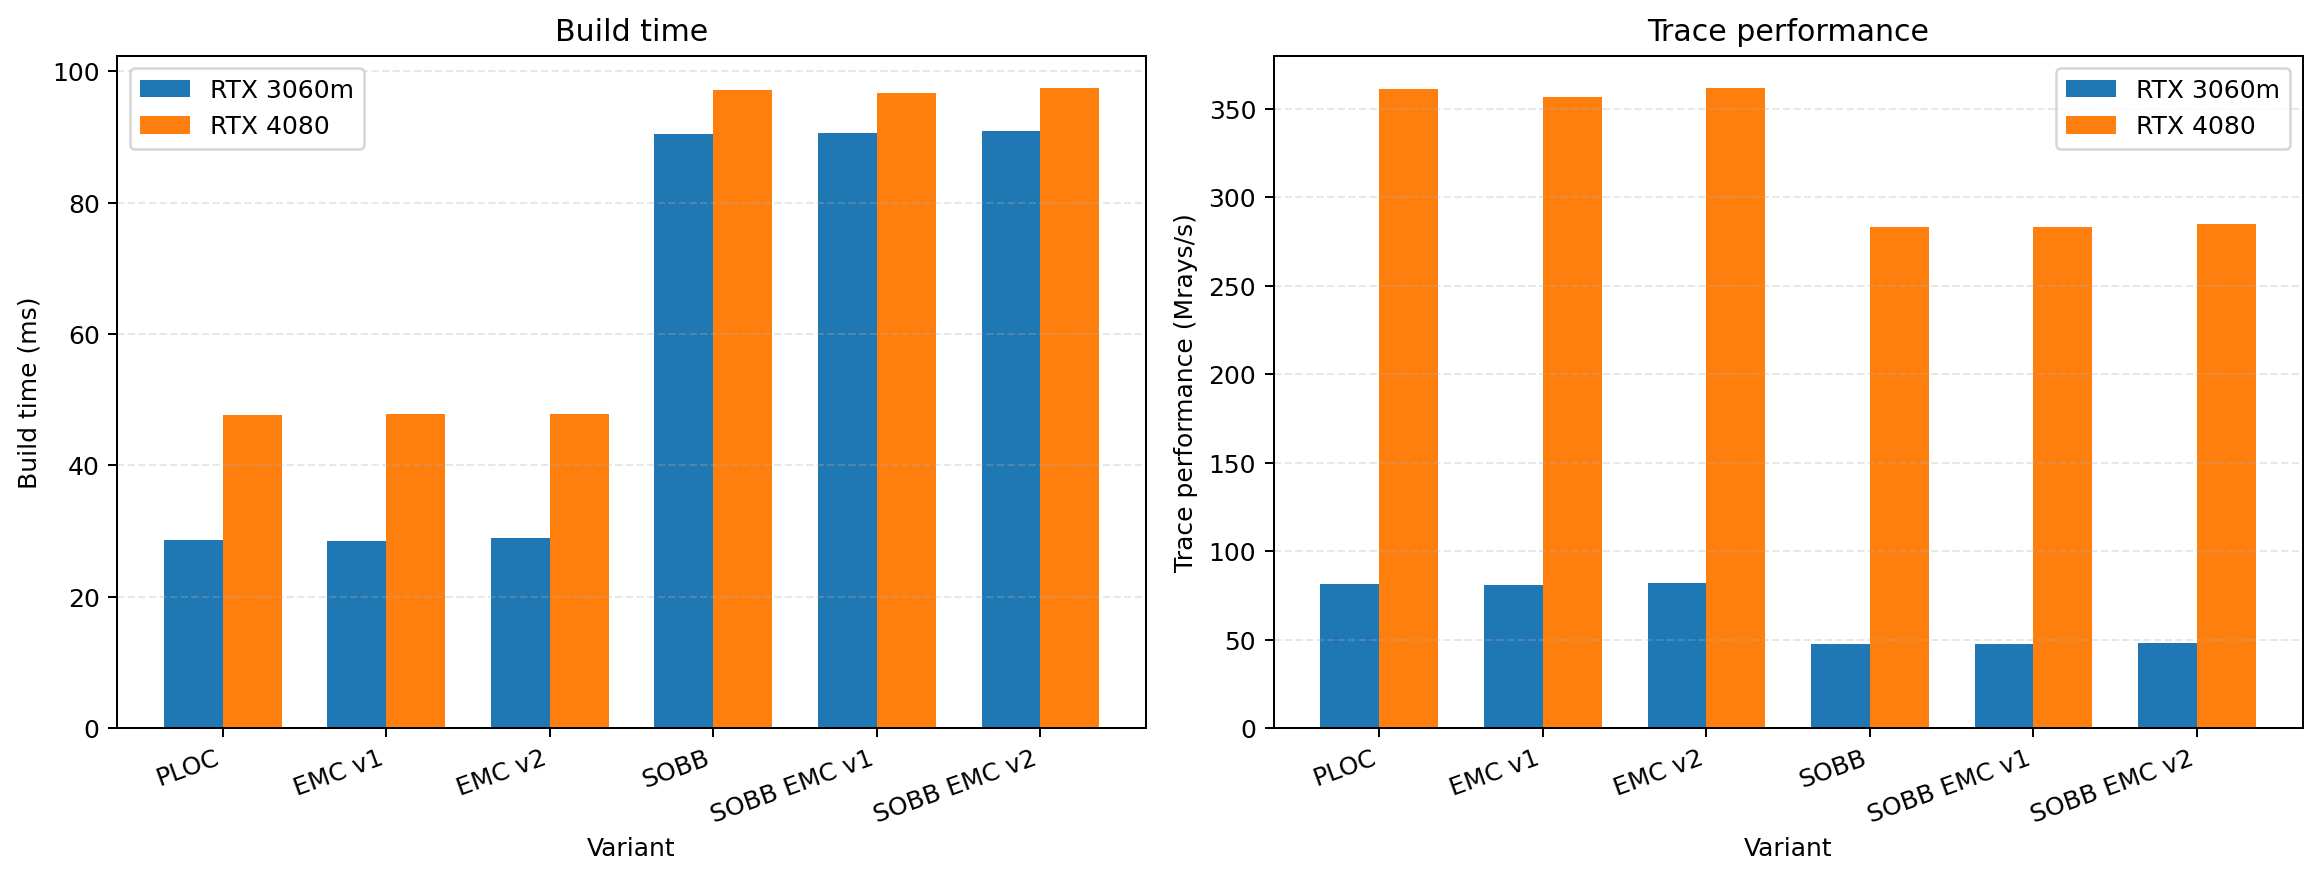
\includegraphics[width=0.95\textwidth]{images/results/graph_gpu_power_comparison.png}
\caption{Comparison of the raw power of the different GPUs and its effect on build time and trace performance.}
\label{fig:gpu-comparison-power}
\end{figure}

The experiments were conducted on two different systems to highlight the impact of hardware performance on the evaluated methods.

The first system was a laptop equipped with an Nvidia GeForce RTX 3060 Mobile GPU with 6~GB of VRAM and an AMD Ryzen 5 5600H CPU. The second system was a desktop workstation featuring an Nvidia GeForce RTX 4080 GPU with 16~GB of VRAM and an Intel Core i7-14700KF CPU.

This dual-platform evaluation allows for a comparison of both absolute performance and scalability across different hardware classes. The differences in BVH construction times and ray tracing throughput (measured in millions of rays per second, MRay/s) between the two systems are illustrated in Figure~\ref{fig:gpu-comparison-power}, where results are averaged across all scenes and camera configurations.

%---------------------------------------------------------------
\section{Scenes}

\begin{table}[!ht]
    \centering
    \small
    \resizebox{\textwidth}{!}{%
    \begin{tabular}{cccc}
        \hline
         Dragon & Hairball & PowerPlant & Rungholt \\
         800k & 2.9M & 12.8M & 5.8M \\
        
        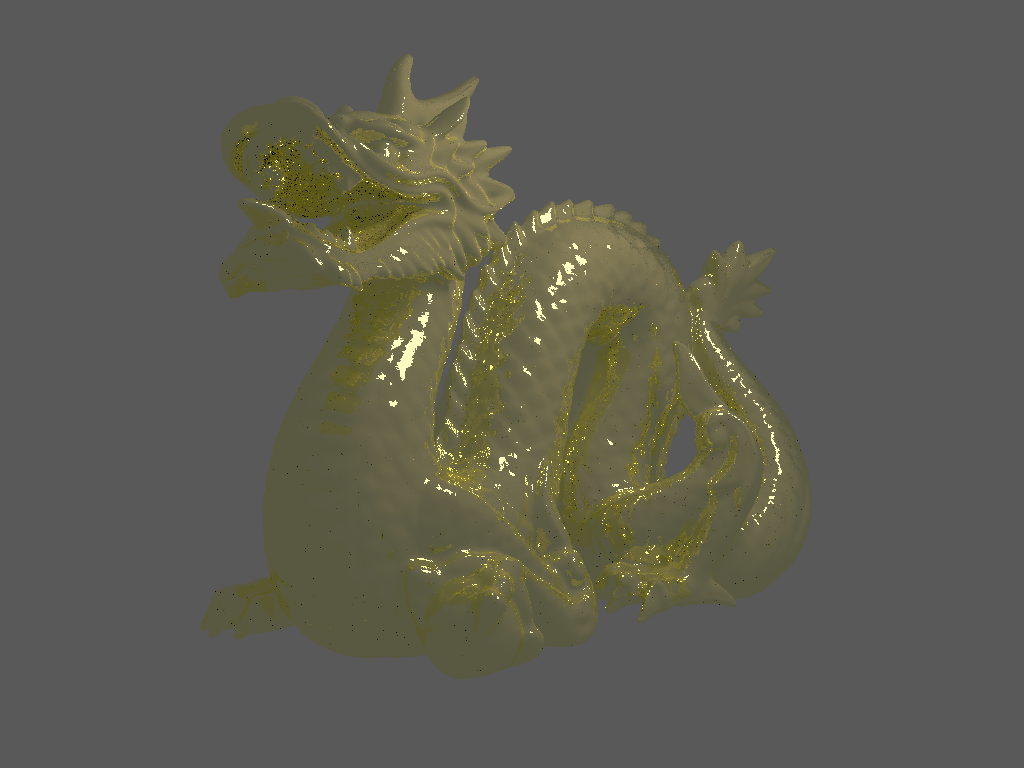
\includegraphics[width=0.25\textwidth]{images/renders/DragonCam0.png} &
        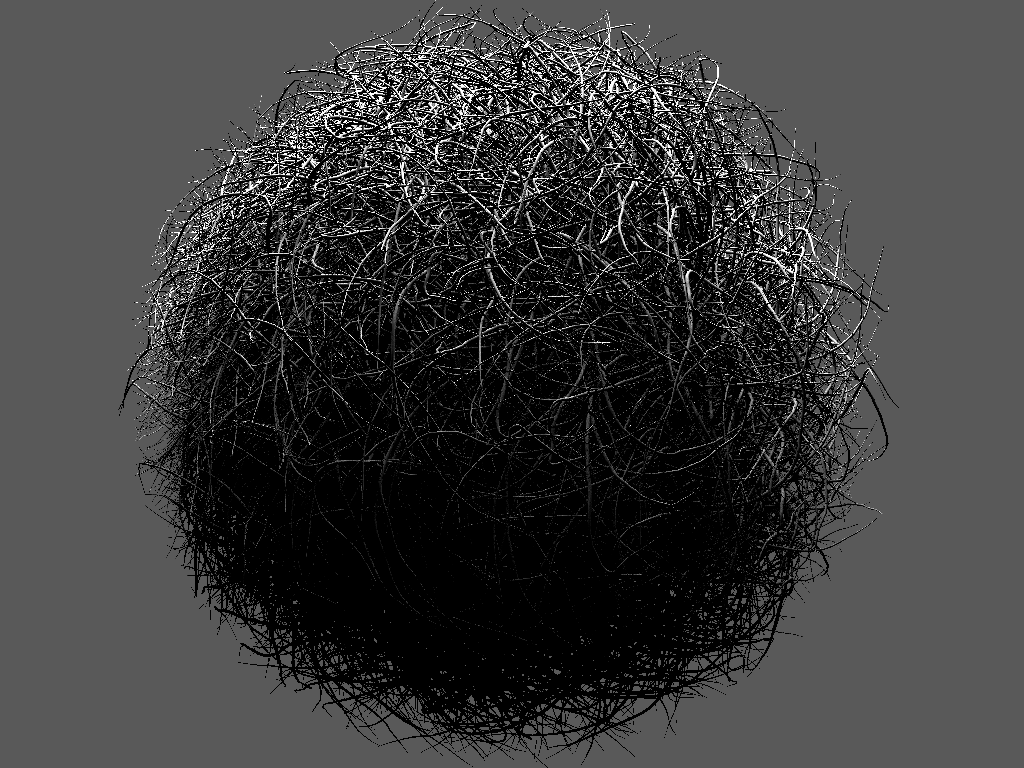
\includegraphics[width=0.25\textwidth]{images/renders/HairballCam0.png} &
        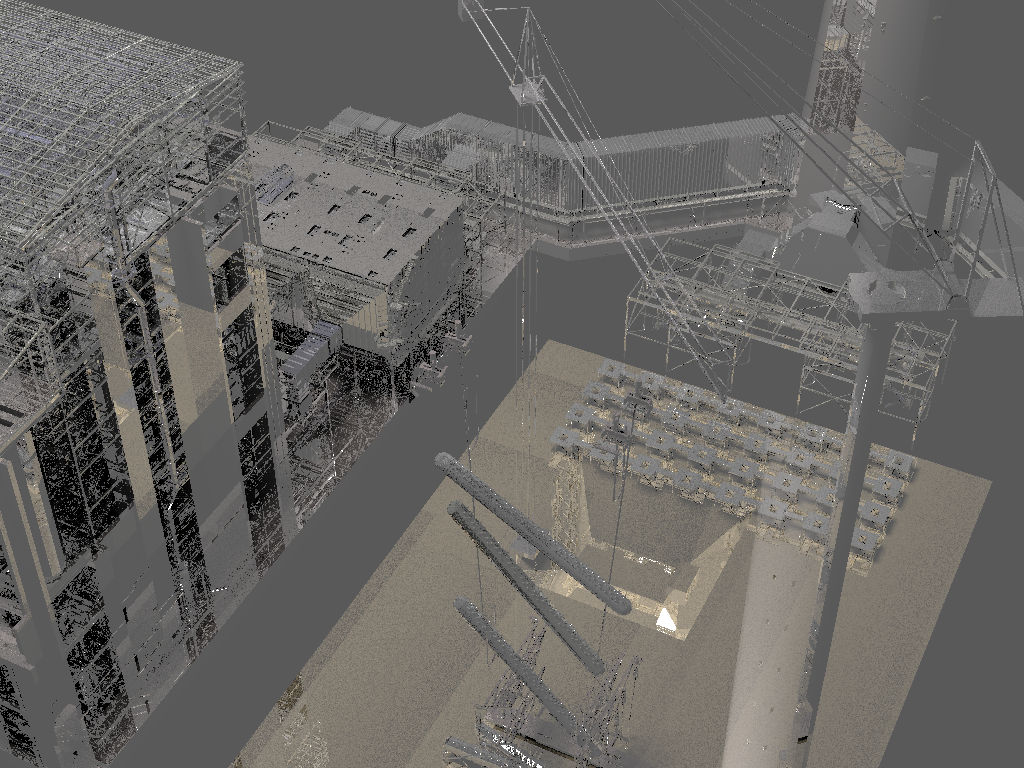
\includegraphics[width=0.25\textwidth]{images/renders/PowerPlantCam0.png} &
        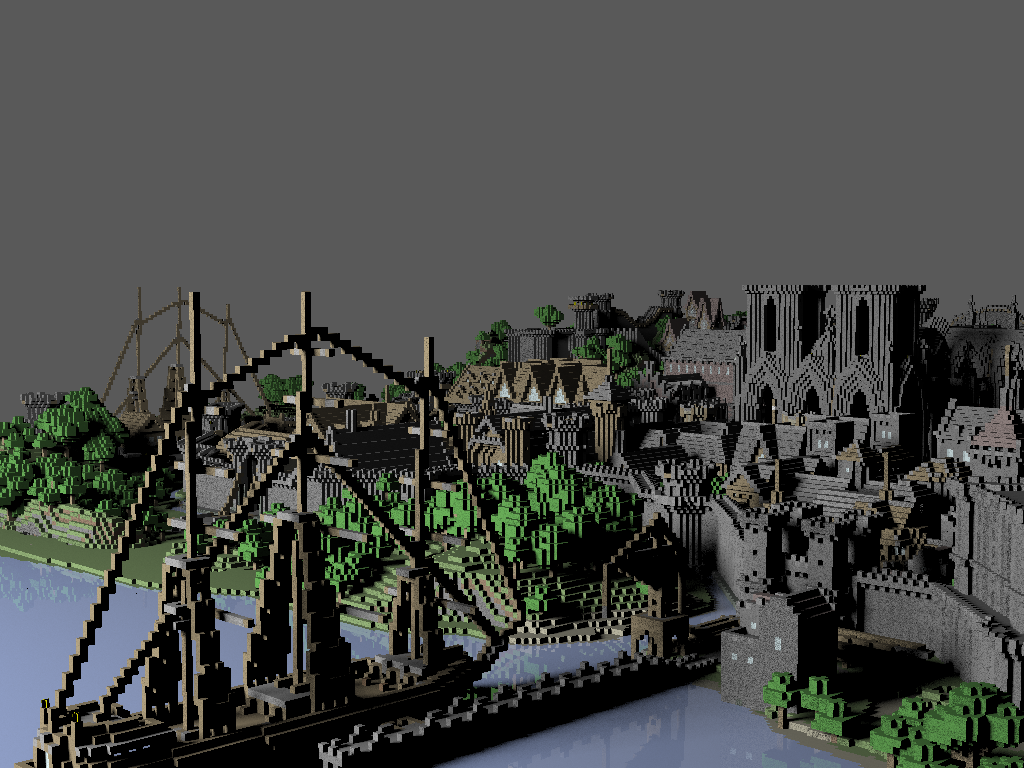
\includegraphics[width=0.25\textwidth]{images/renders/RungholtCam0.png} \\
        
        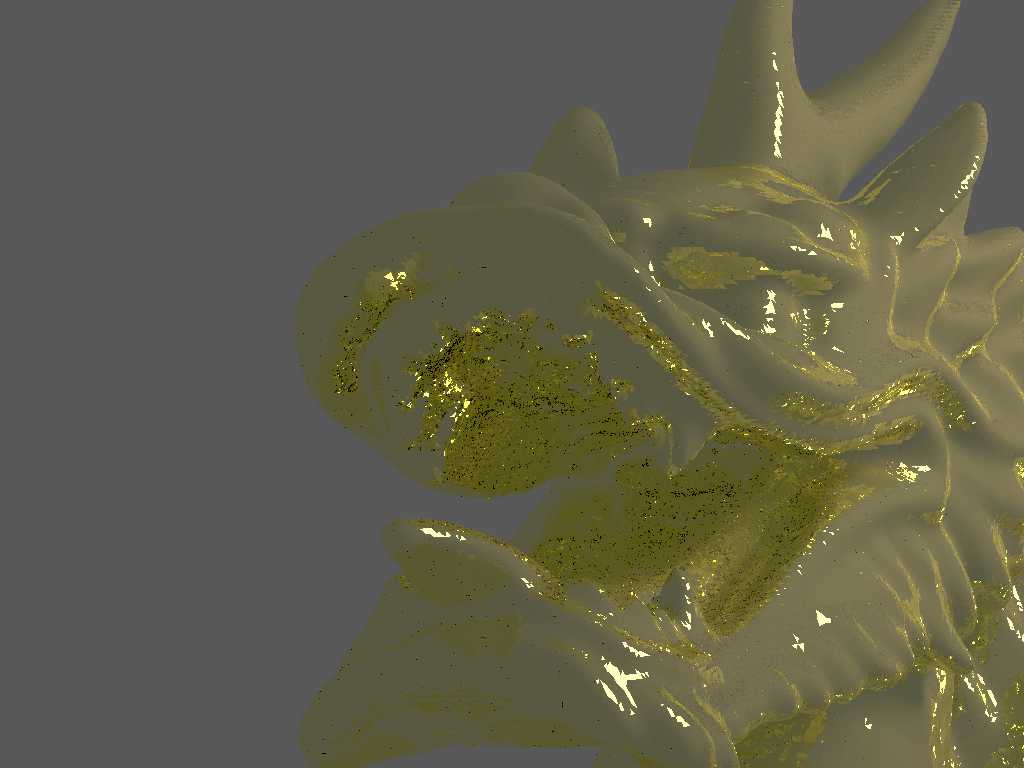
\includegraphics[width=0.25\textwidth]{images/renders/DragonCam1.png} &
        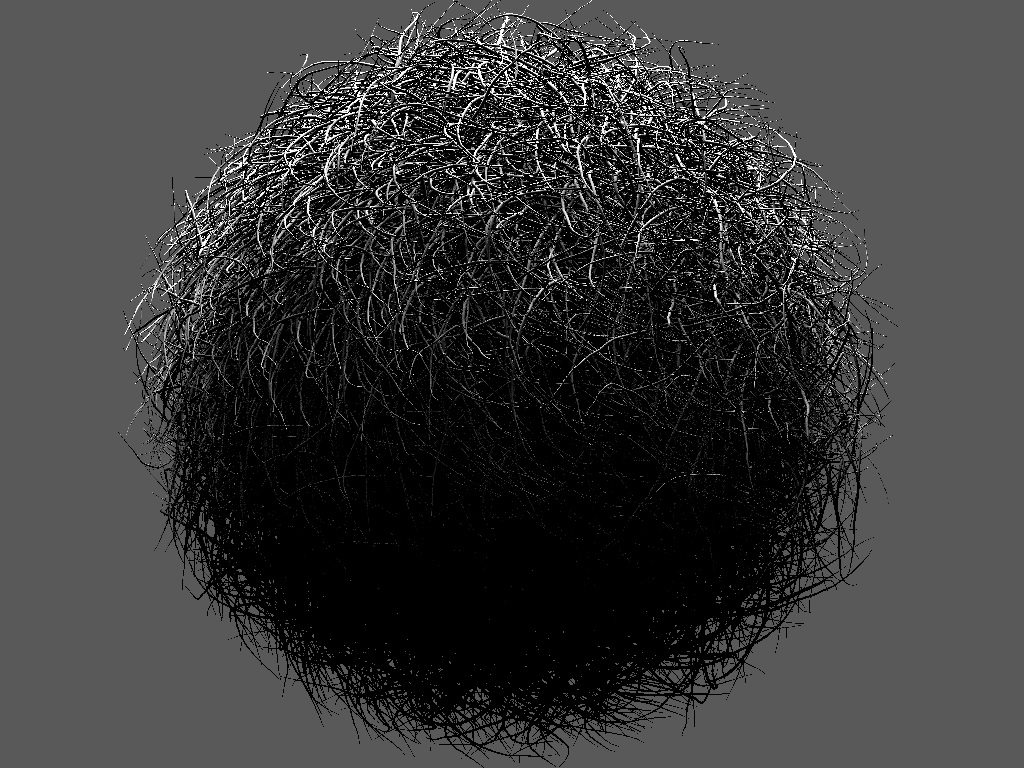
\includegraphics[width=0.25\textwidth]{images/renders/HairballCam1.png} &
        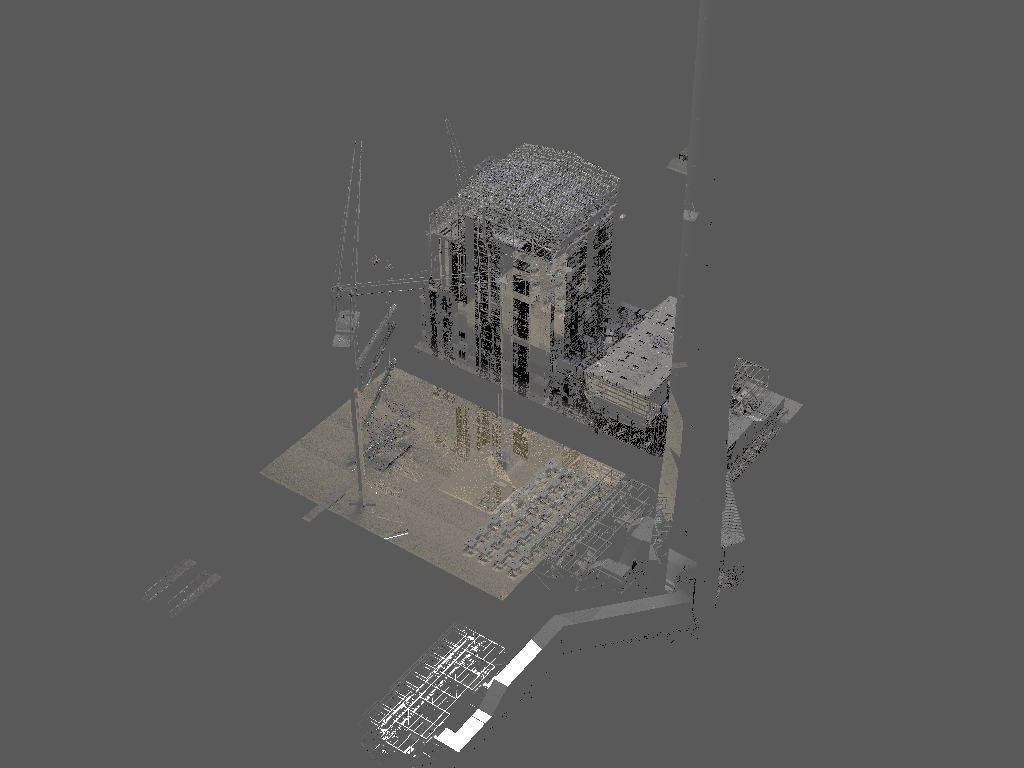
\includegraphics[width=0.25\textwidth]{images/renders/PowerPlantCam1.png} &
        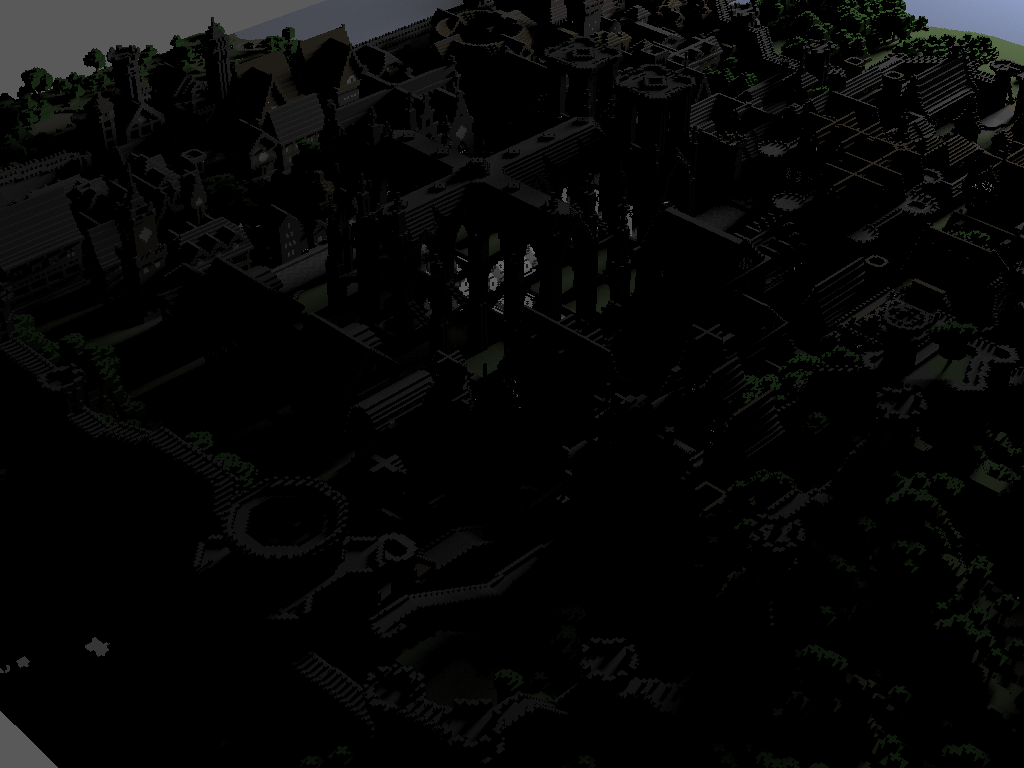
\includegraphics[width=0.25\textwidth]{images/renders/RungholtCam1.png} \\
        
        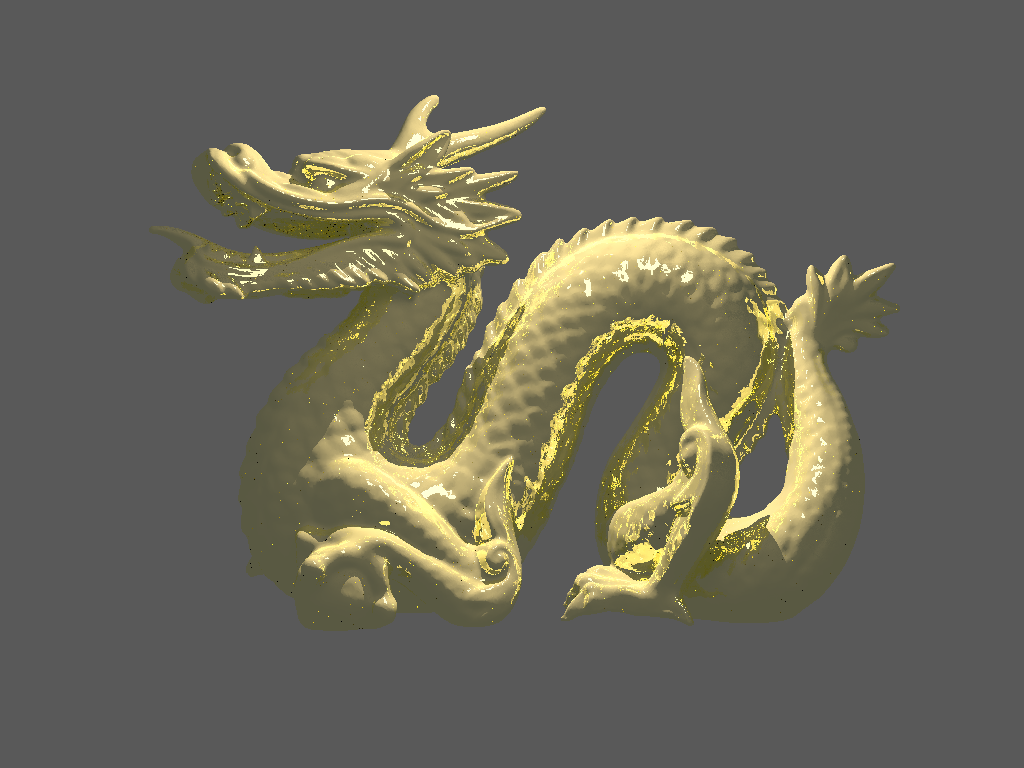
\includegraphics[width=0.25\textwidth]{images/renders/DragonCam2.png} &
        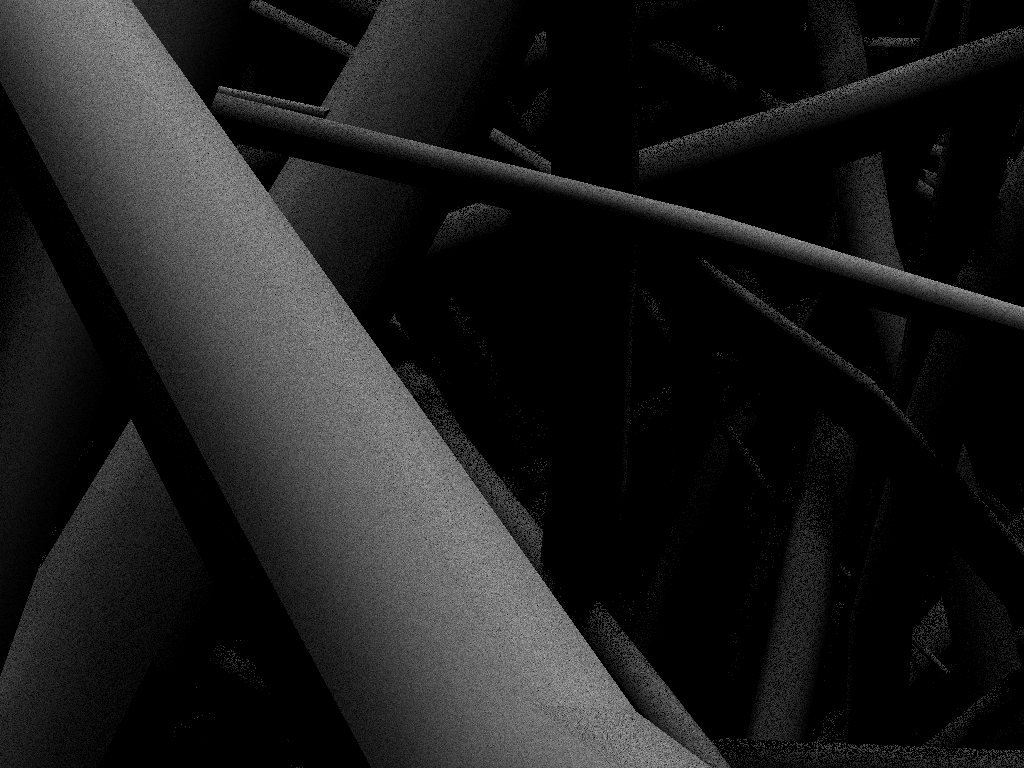
\includegraphics[width=0.25\textwidth]{images/renders/HairballCam2.png} &
        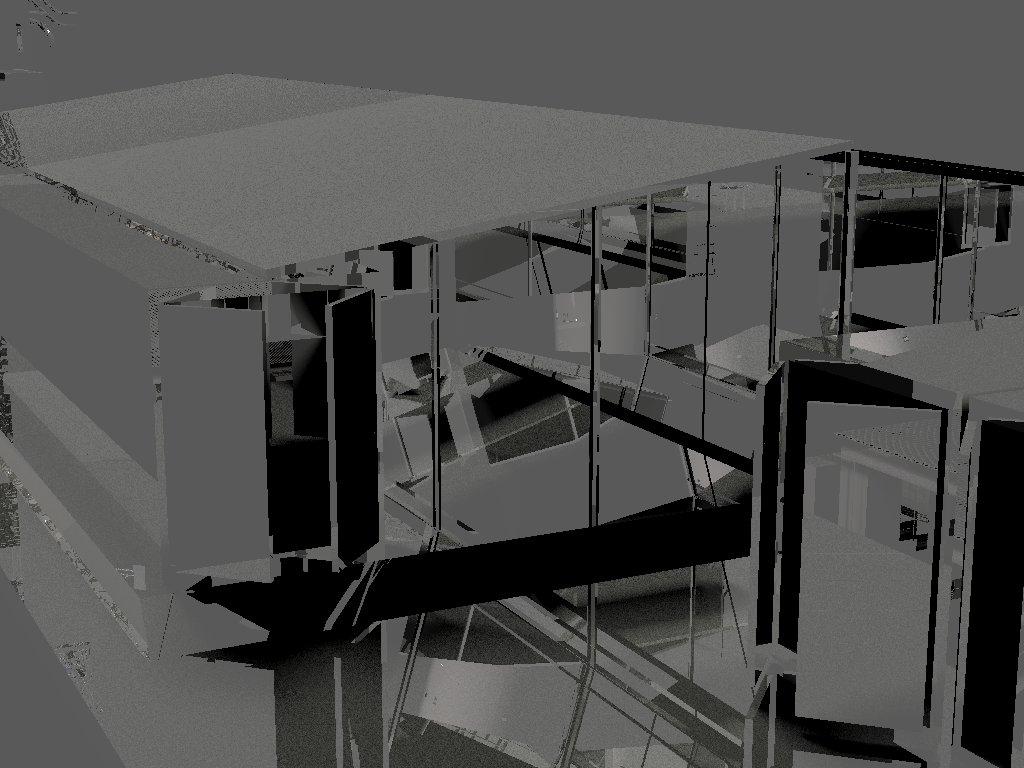
\includegraphics[width=0.25\textwidth]{images/renders/PowerPlantCam2.png} &
        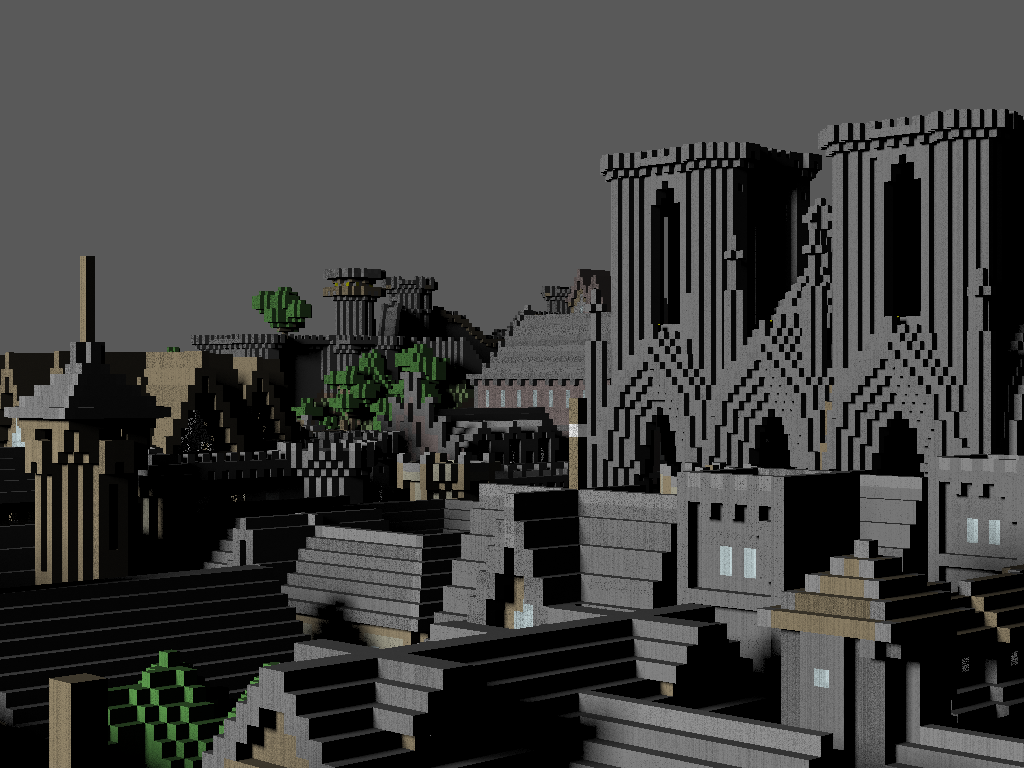
\includegraphics[width=0.25\textwidth]{images/renders/RungholtCam2.png} \\
         Skydemo & Sponza & Stegosaurus & Venlo \\
         3.7M & 262k & 5.7M & 1.3M \\
        
        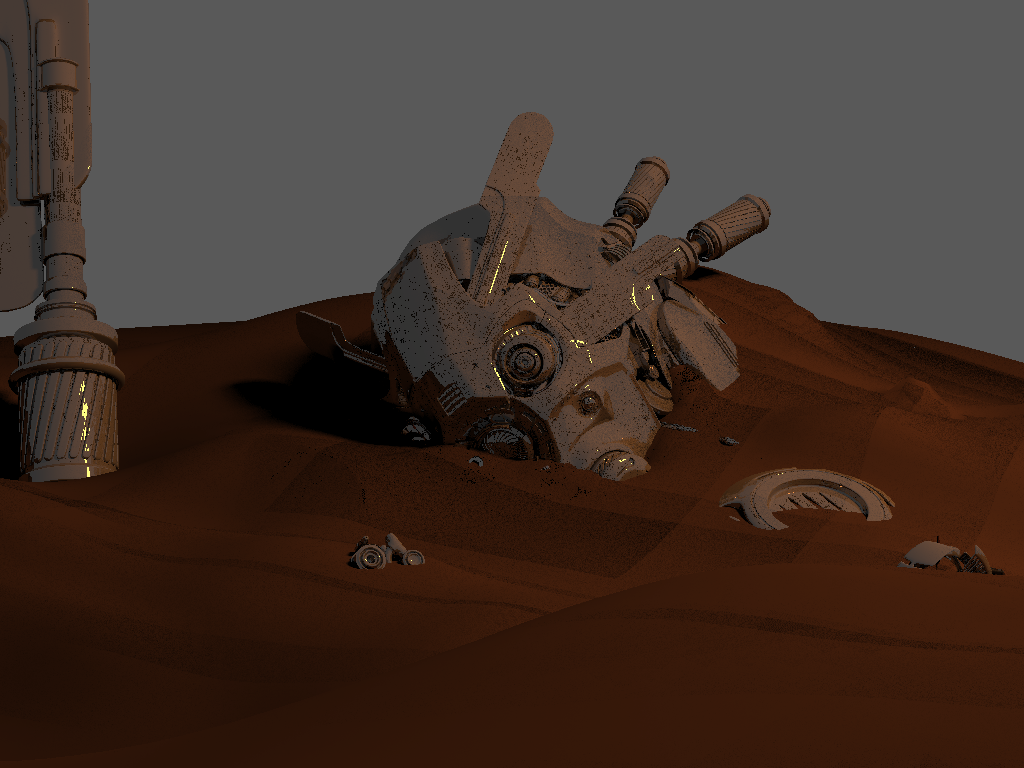
\includegraphics[width=0.25\textwidth]{images/renders/SkydemoCam0.png} &
        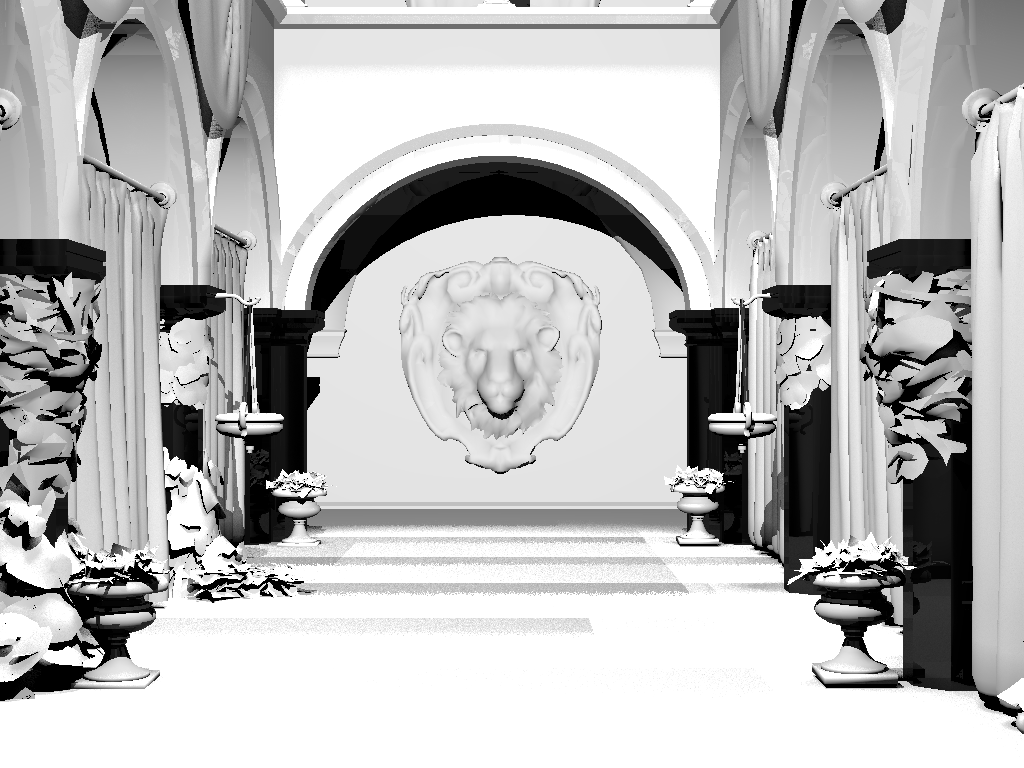
\includegraphics[width=0.25\textwidth]{images/renders/SponzaCam0.png} &
        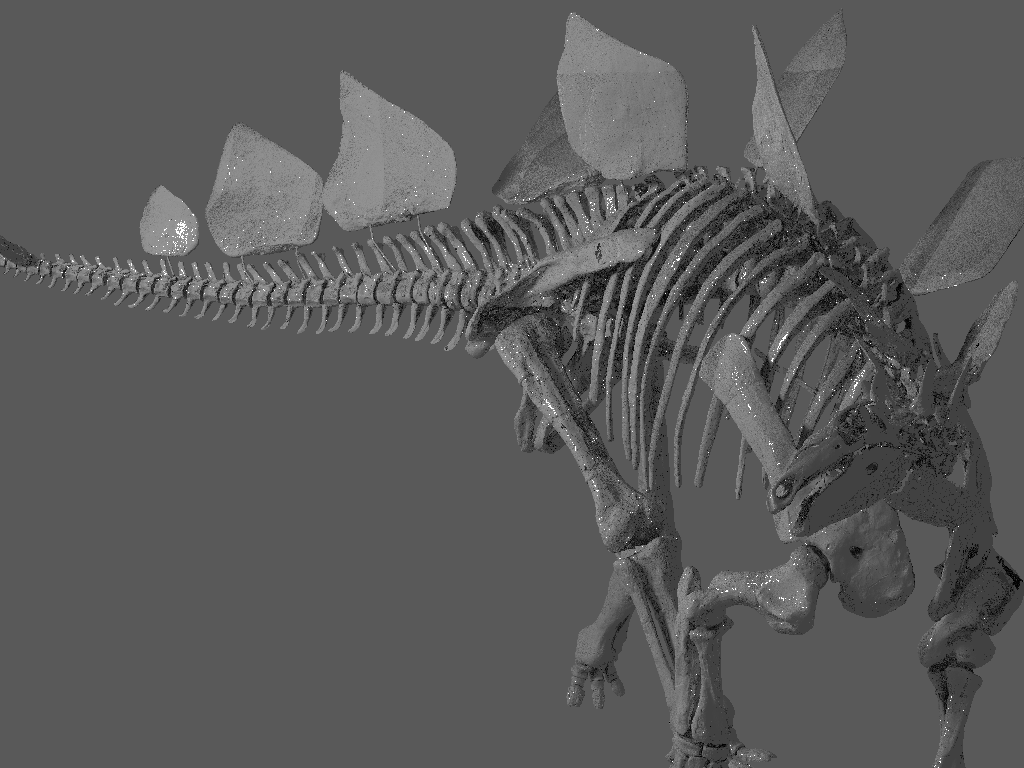
\includegraphics[width=0.25\textwidth]{images/renders/StegosaurusCam0.png} &
        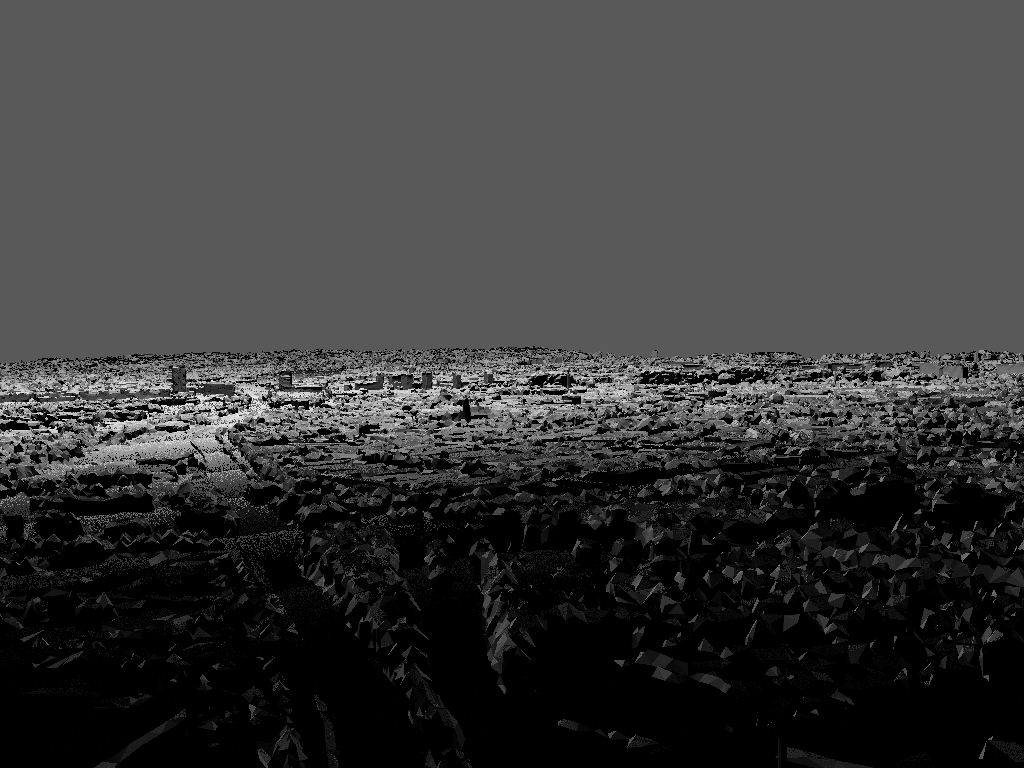
\includegraphics[width=0.25\textwidth]{images/renders/VenloCam0.png} \\
        
        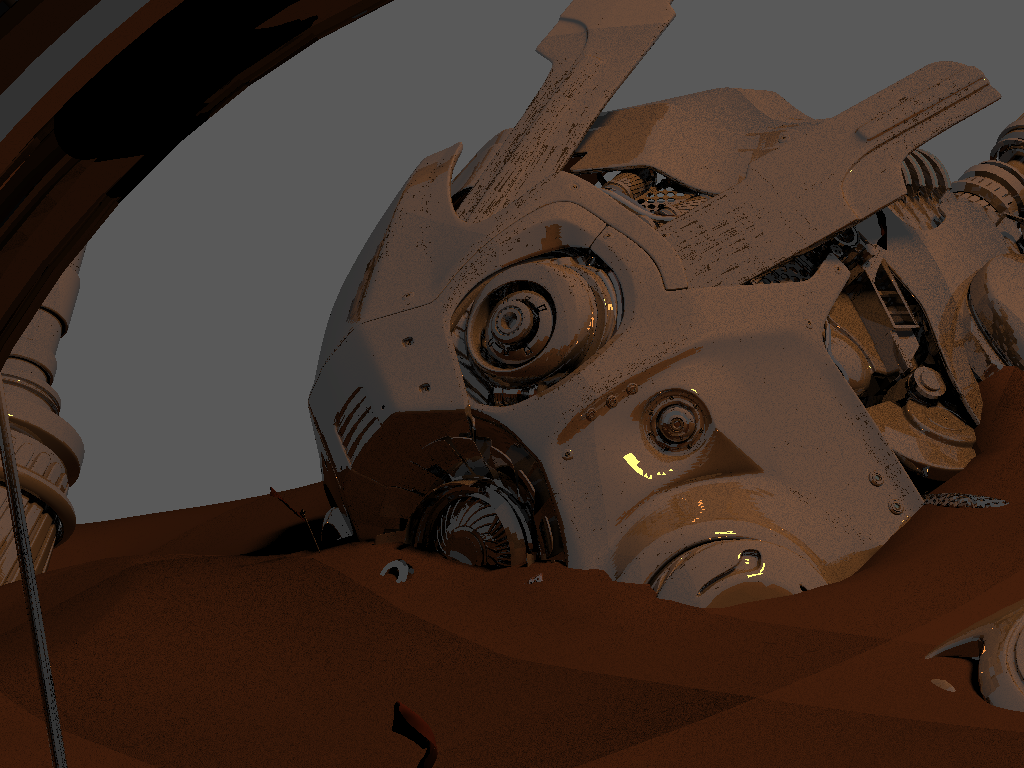
\includegraphics[width=0.25\textwidth]{images/renders/SkydemoCam1.png} &
        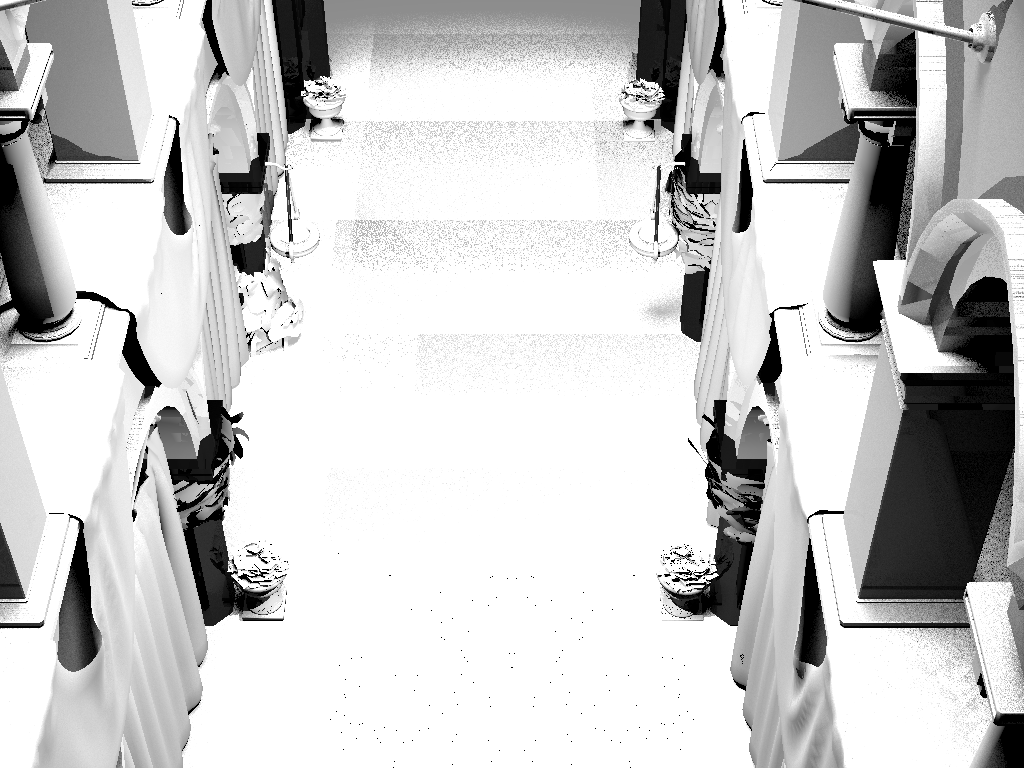
\includegraphics[width=0.25\textwidth]{images/renders/SponzaCam1.png} &
        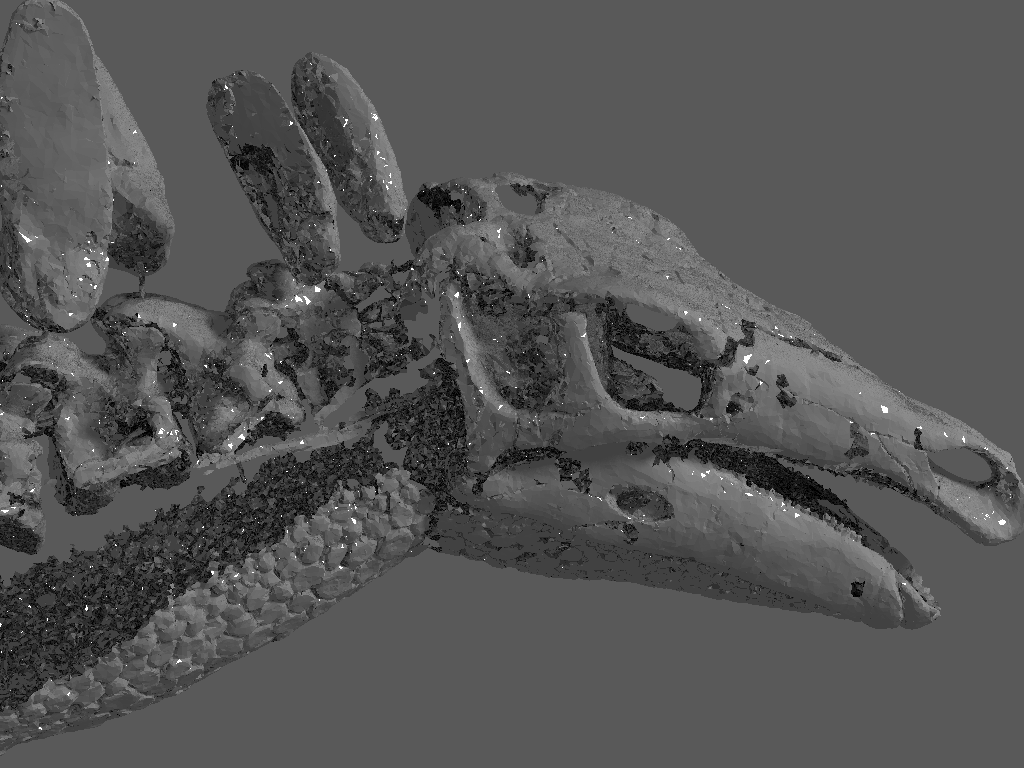
\includegraphics[width=0.25\textwidth]{images/renders/StegosaurusCam1.png} &
        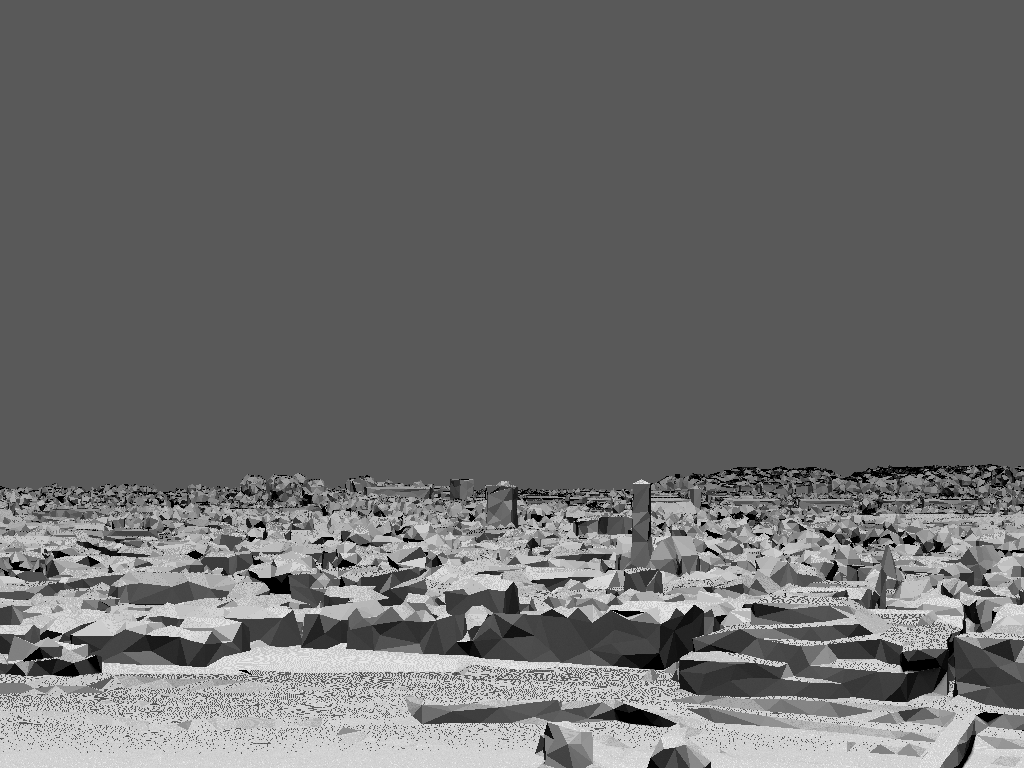
\includegraphics[width=0.25\textwidth]{images/renders/VenloCam1.png} \\
        
        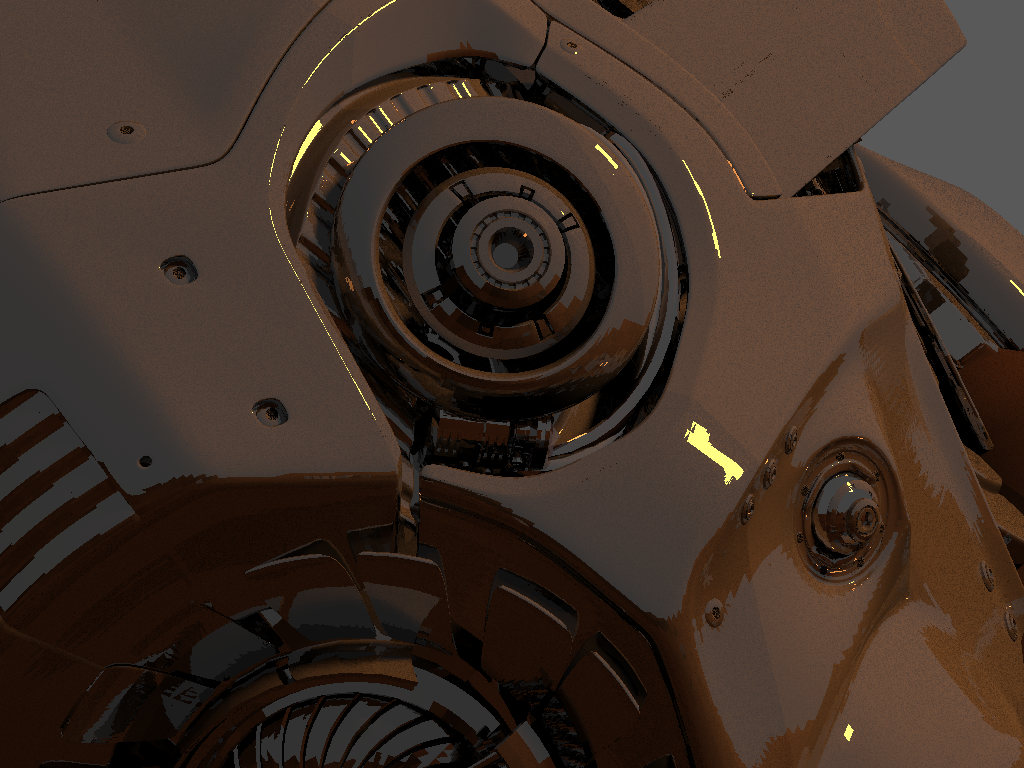
\includegraphics[width=0.25\textwidth]{images/renders/SkydemoCam2.png} &
        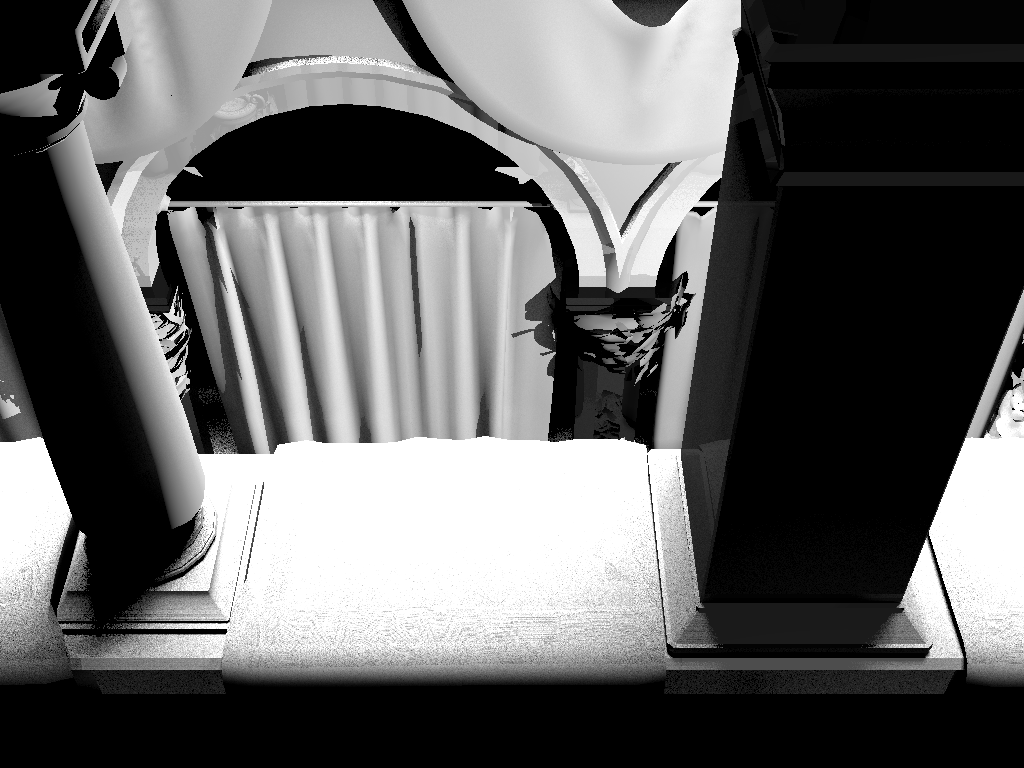
\includegraphics[width=0.25\textwidth]{images/renders/SponzaCam2.png} &
        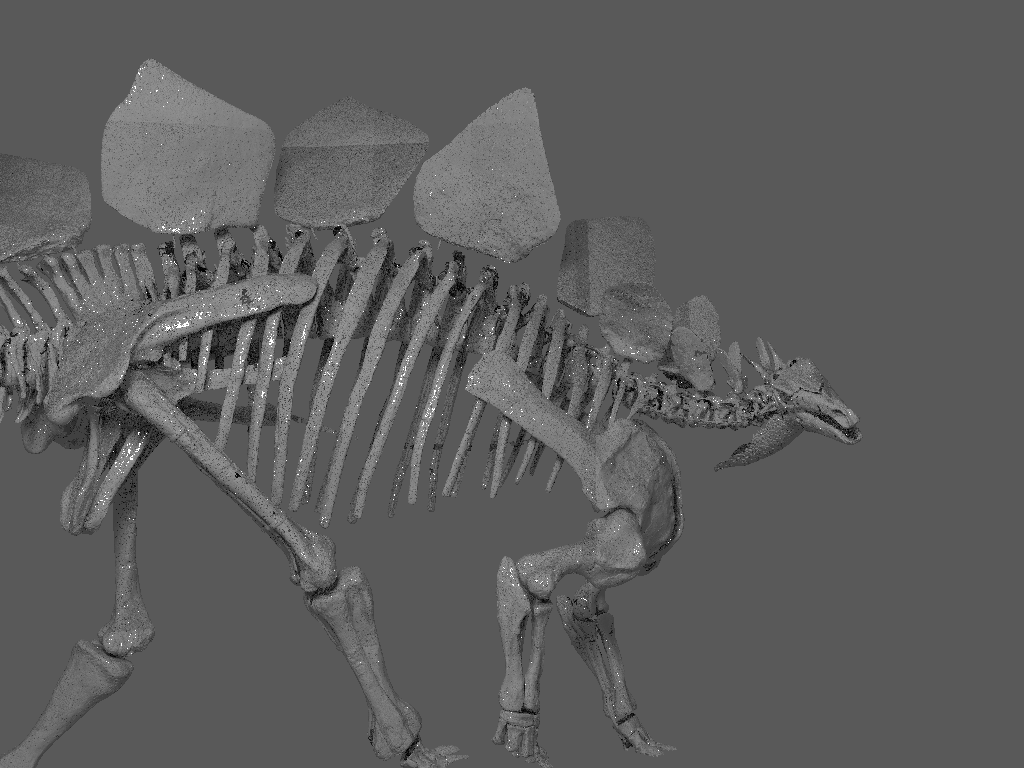
\includegraphics[width=0.25\textwidth]{images/renders/StegosaurusCam2.png} &
        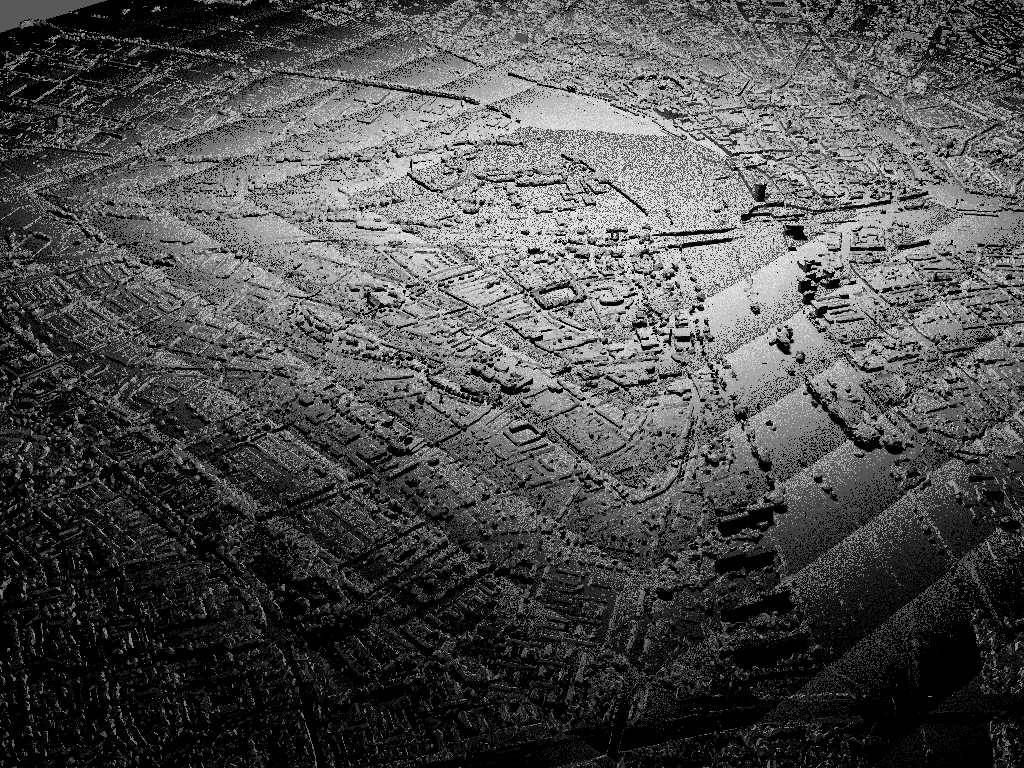
\includegraphics[width=0.25\textwidth]{images/renders/VenloCam2.png} \\
        \hline
    \end{tabular}
    }
    \caption{Rendered images of the 8 tested scenes in resolution $1024 \times 768$. Three representative views were used for each scene.}
    \label{tab:final-renders}
\end{table}

A total of 8 scenes were selected for evaluation, each rendered from 3 different camera viewpoints. These scenes were chosen to represent a diverse set of geometric complexity, spatial distribution, and visibility conditions, ensuring that the evaluated methods are tested under varying workloads.

For each scene and camera configuration, the rendering process generates a combination of primary rays, secondary rays (reflections and refractions), and shadow rays. The proportion of these ray types varies depending on scene composition, material properties, and camera placement, which directly influences the performance characteristics of the evaluated acceleration structures.

\begin{table}[!ht]
    \small
    \centering
    \resizebox{\textwidth}{!}{%
    \begin{tabular}{llccc}
        \hline
        Scene & Camera & Primary [Mrays] & Secondary [Mrays] & Shadow [Mrays] \\
        \hline

        \multirow{3}{*}{\shortstack{Dragon \\ \# of triangles: 800k}}
        & cam0 & 25.17 (30.95\%) & 11.23 (13.81\%) & 44.92 (55.24\%) \\
        & cam1 & 25.17 (16.87\%) & 24.81 (16.63\%) & 99.23 (66.51\%) \\
        & cam2 & 25.17 (27.97\%) & 10.80 (12.00\%) & 54.01 (60.02\%) \\

        \hline
        \multirow{3}{*}{\shortstack{Hairball \\ \# of triangles: 2.9M}}
        & cam0 & 25.17 (34.06\%) & 0.00 (0.00\%) & 48.72 (65.94\%) \\
        & cam1 & 25.17 (33.65\%) & 0.00 (0.00\%) & 49.63 (66.35\%) \\
        & cam2 & 25.17 (20.00\%) & 0.00 (0.00\%) & 100.66 (80.00\%) \\

        \hline
        \multirow{3}{*}{\shortstack{PowerPlant \\ \# of triangles: 12.8M}}
        & cam0 & 25.17 (8.69\%) & 52.86 (18.26\%) & 211.45 (73.05\%) \\
        & cam1 & 25.17 (27.00\%) & 13.61 (14.60\%) & 54.44 (58.40\%) \\
        & cam2 & 25.17 (5.34\%) & 89.30 (18.93\%) & 357.20 (75.73\%) \\

        \hline
        \multirow{3}{*}{\shortstack{Rungholt \\ \# of triangles: 5.8M}}
        & cam0 & 25.17 (28.71\%) & 1.73 (1.97\%) & 60.77 (69.32\%) \\
        & cam1 & 25.17 (19.74\%) & 1.02 (0.80\%) & 101.29 (79.46\%) \\
        & cam2 & 25.17 (26.12\%) & 0.46 (0.48\%) & 70.73 (73.40\%) \\

        \hline
        \multirow{3}{*}{\shortstack{Skydemo \\ \# of triangles: 3.7M}}
        & cam0 & 25.17 (21.71\%) & 7.56 (6.52\%) & 83.20 (71.77\%) \\
        & cam1 & 25.17 (14.22\%) & 21.90 (12.37\%) & 129.90 (73.41\%) \\
        & cam2 & 25.17 (9.84\%) & 40.41 (15.80\%) & 190.15 (74.36\%) \\

        \hline
        \multirow{3}{*}{\shortstack{Sponza \\ \# of triangles: 262k}}
        & cam0 & 25.17 (10.92\%) & 13.27 (5.76\%) & 191.93 (83.32\%) \\
        & cam1 & 25.17 (12.27\%) & 9.14 (4.45\%) & 170.77 (83.27\%) \\
        & cam2 & 25.17 (11.63\%) & 10.92 (5.05\%) & 180.35 (83.33\%) \\

        \hline
        \multirow{3}{*}{\shortstack{Stegosaurus \\ \# of triangles: 5.7M}}
        & cam0 & 25.17 (24.78\%) & 15.28 (15.04\%) & 61.11 (60.18\%) \\
        & cam1 & 25.17 (15.32\%) & 27.82 (16.94\%) & 111.28 (67.74\%) \\
        & cam2 & 25.17 (23.77\%) & 16.14 (15.25\%) & 64.56 (60.98\%) \\

        \hline
        \multirow{3}{*}{\shortstack{Venlo \\ \# of triangles: 1.3M}}
        & cam0 & 25.17 (31.64\%) & 0.00 (0.00\%) & 54.36 (68.36\%) \\
        & cam1 & 25.17 (39.93\%) & 0.00 (0.00\%) & 37.86 (60.07\%) \\
        & cam2 & 25.17 (20.04\%) & 0.00 (0.00\%) & 100.44 (79.96\%) \\

        \hline
    \end{tabular}
    }
    \caption{Ray distribution per scene and camera. Ray counts are shown in millions (Mrays), with percentage share in parentheses.}
    \label{tab:ray-distribution}
\end{table}

To provide visual context, the final rendered images of all scenes are presented in Table~\ref{tab:final-renders}. Additionally, a detailed breakdown of ray counts, including their absolute values and relative percentages of the total ray count, is provided in Table~\ref{tab:ray-distribution} along with the triangle counts for each scene. This information is important for understanding how different ray types contribute to the overall workload and how they may impact traversal performance.

As in the overall experimental setup, each scene and camera combination was evaluated 5 times, and the median value was used to mitigate the effect of random performance fluctuations.

Most of the scenes are courtesy of Morgan McGuire's archive \cite{McGuire2017}. The Stegosaurus scene was taken from the Smithsonian institution's 3D render archive \cite{si}. The Skydemo scene is part of the Blender demo files \cite{blender_demo}.

%---------------------------------------------------------------
\clearpage
\newpage
\section{Results}

\begin{figure}[h!tb]
\centering
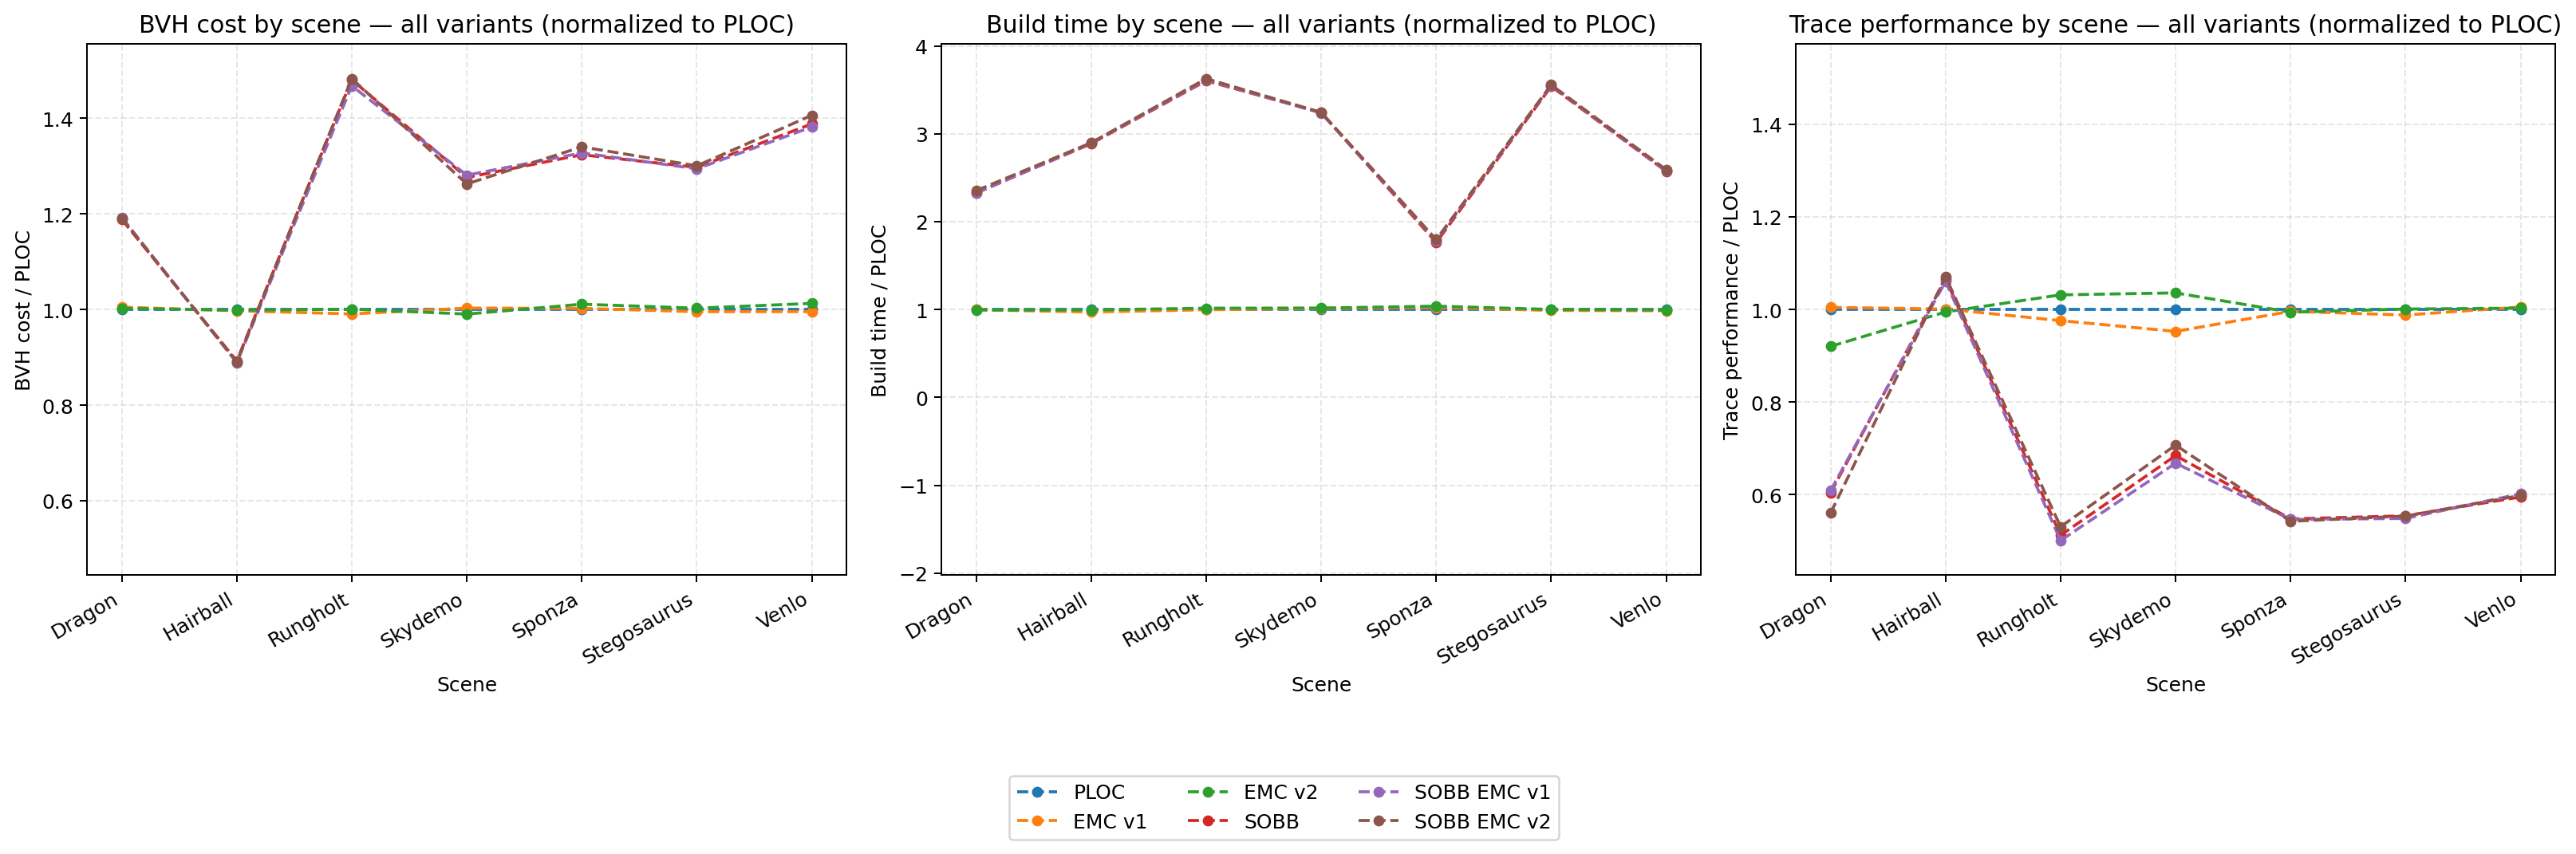
\includegraphics[width=0.95\textwidth]{images/results/rtx3060mobile/graph_scene_statistics_all_variants_normalized.png}
\caption{BVH cost, build time (in ms) and traversal performance (in Mrays/s) per scene, relative to the PLOC variant. Nvidia RTX 3060 Mobile.}
\label{fig:scene-statistics-all-variants-3060}
\end{figure}

\begin{figure}[h!tb]
\centering

\includegraphics[width=0.95\textwidth]{images/results/rtx4080/graph_scene_statistics_all_variants_normalized.png}
\caption{BVH cost, build time (in ms) and traversal performance (in Mrays/s) per scene, relative to the PLOC variant. Nvidia RTX 4080.}
\label{fig:scene-statistics-all-variants-4080}
\end{figure}

Figures~\ref{fig:scene-statistics-all-variants-3060} and \ref{fig:scene-statistics-all-variants-4080} present an overview of the measured results for the Nvidia GeForce RTX 3060 Mobile and Nvidia GeForce RTX 4080, respectively. These figures summarize three key metrics: BVH cost, construction time (in milliseconds), and traversal performance (in millions of rays per second, MRay/s). For clarity, all values are expressed relative to the baseline PLOC variant.

Each data point represents an average across all scenes and camera configurations. While this aggregated view provides a general comparison of the evaluated methods, it also reveals that some variants exhibit very similar performance characteristics. In particular, the PLOC, EMC v1, and EMC v2 variants tend to produce closely clustered results, as do the SOBB-based variants. As a consequence, differences between individual methods are less distinguishable in these combined plots.

\begin{figure}[h!tb]
\centering
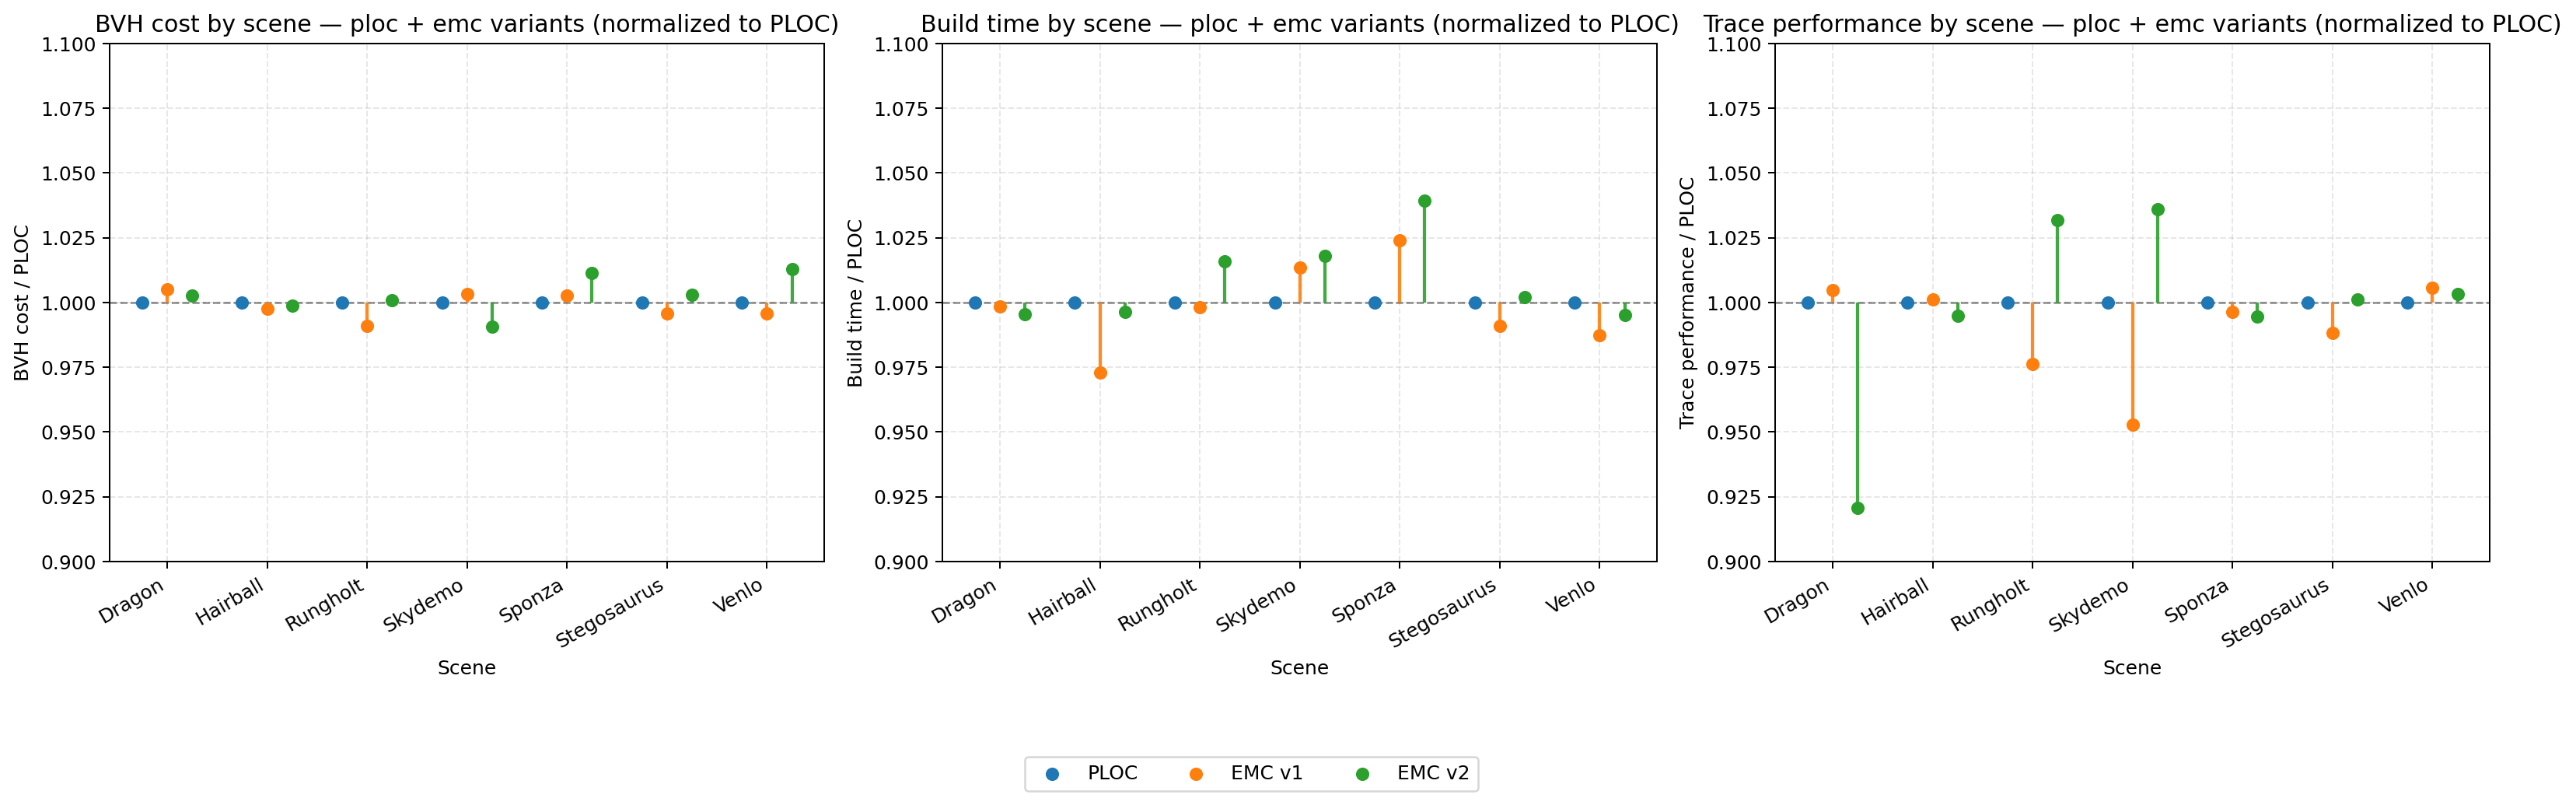
\includegraphics[width=0.95\textwidth]{images/results/rtx3060mobile/graph_scene_statistics_ploc_emc_normalized.png}
\caption{BVH cost, build time (in ms) and traversal performance (in Mrays/s) per scene for PLOC, PLOC EMC v1 and PLOC EMC v2 variants, relative to the PLOC variant. Nvidia RTX 3060 Mobile.}
\label{fig:scene-statistics-emc-3060}
\end{figure}

\begin{figure}[h!tb]
\centering

\includegraphics[width=0.95\textwidth]{images/results/rtx4080/graph_scene_statistics_ploc_emc_normalized.png}
\caption{BVH cost, build time (in ms) and traversal performance (in Mrays/s) per scene for PLOC, PLOC EMC v1 and PLOC EMC v2 variants, relative to the PLOC variant. Nvidia RTX 4080.}
\label{fig:scene-statistics-emc-4080}
\end{figure}

To improve readability and enable a more detailed comparison, the results are further divided into two groups. Figures~\ref{fig:scene-statistics-emc-3060} and \ref{fig:scene-statistics-emc-4080} focus on the baseline and EMC-enhanced variants (PLOC, EMC v1, EMC v2), with all values normalized relative to the PLOC baseline. Similarly, Figures~\ref{fig:scene-statistics-sobb-3060} and \ref{fig:scene-statistics-sobb-4080} present the SOBB-based variants (SOBB, SOBB EMC v1, SOBB EMC v2), normalized relative to the SOBB baseline.

\begin{figure}[h!tb]
\centering
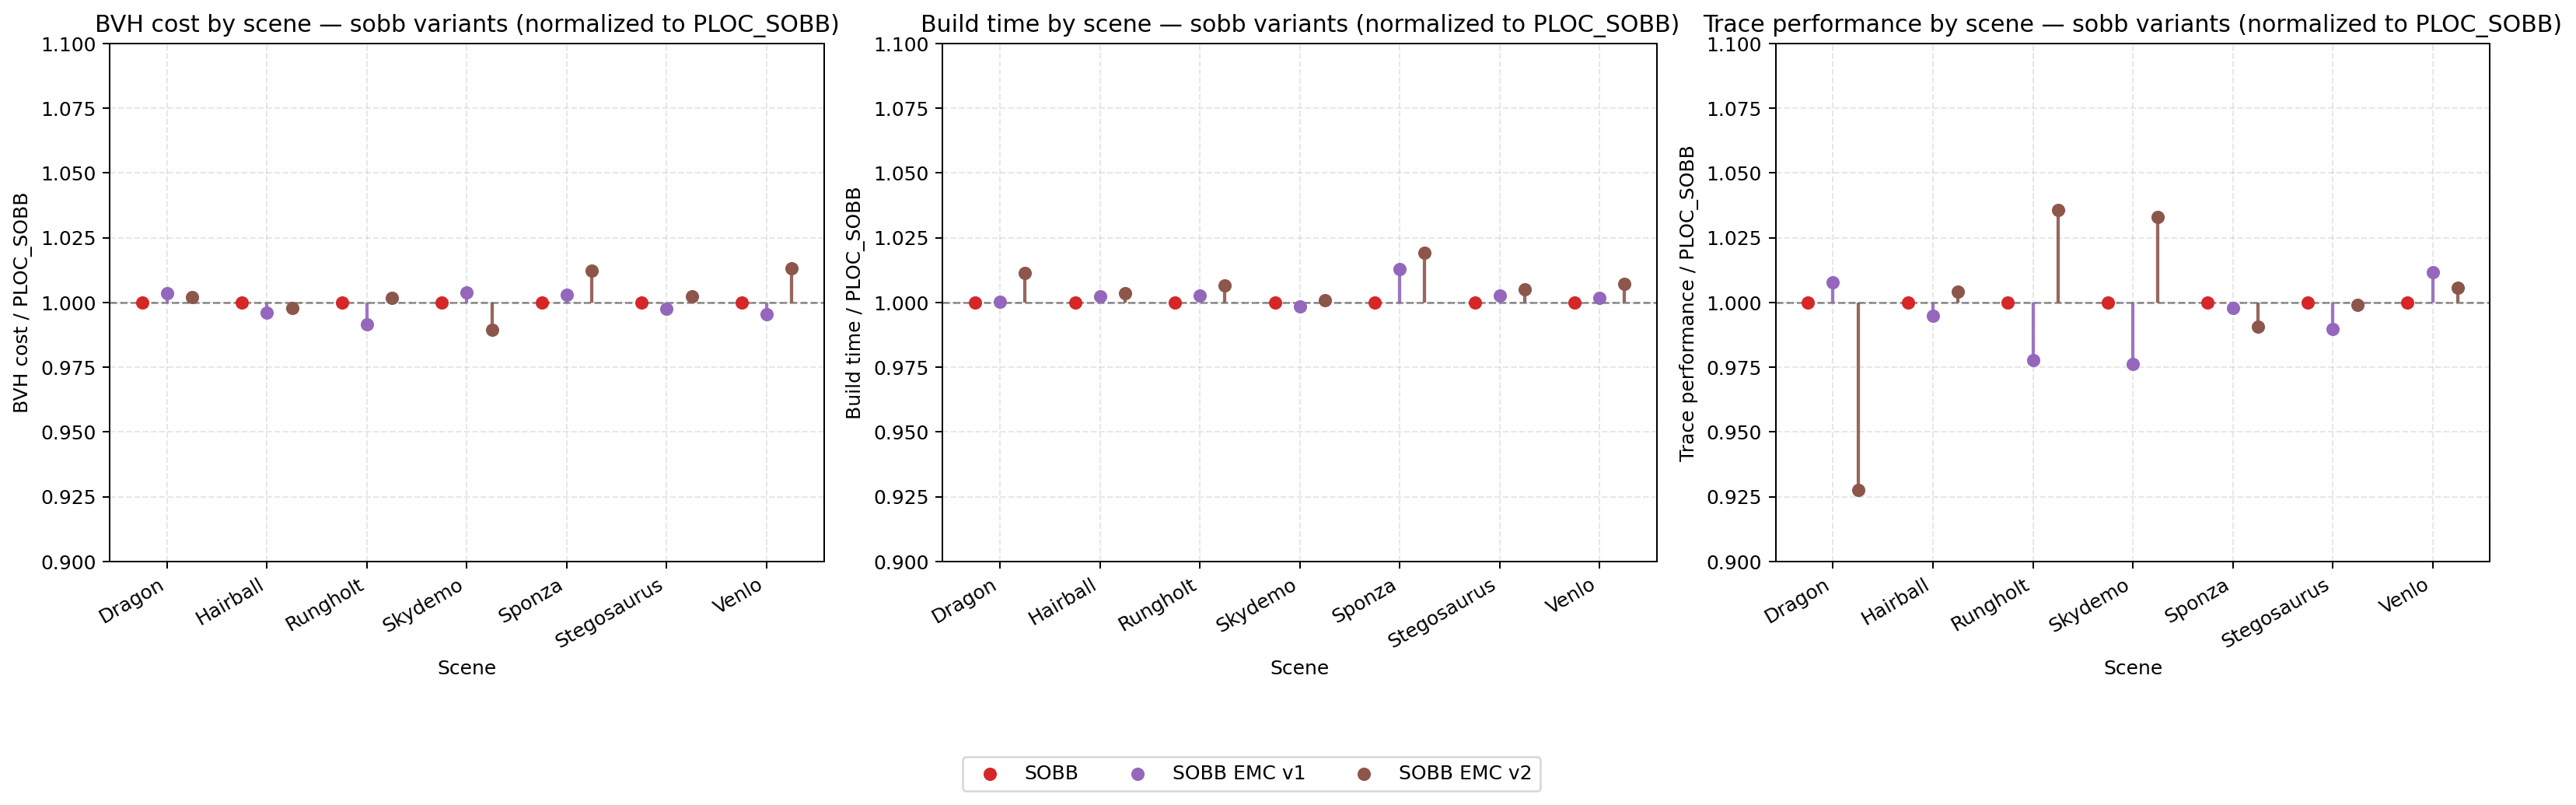
\includegraphics[width=0.95\textwidth]{images/results/rtx3060mobile/graph_scene_statistics_sobb_normalized.png}
\caption{BVH cost, build time (in ms) and traversal performance (in Mrays/s) per scene for SOBB, SOBB EMC v1 and SOBB EMC v2 variants, relative to the SOBB variant. Nvidia RTX 3060 Mobile.}
\label{fig:scene-statistics-sobb-3060}
\end{figure}

\begin{figure}[h!tb]
\centering

\includegraphics[width=0.95\textwidth]{images/results/rtx4080/graph_scene_statistics_sobb_normalized.png}
\caption{BVH cost, build time (in ms) and traversal performance (in Mrays/s) per scene for SOBB, SOBB EMC v1 and SOBB EMC v2 variants, relative to the SOBB variant. Build time for the Sponza scene for the SOBB EMC v2 variant is an outlier and thus the graph is not scaled to see its true values. Nvidia RTX 4080.}
\label{fig:scene-statistics-sobb-4080}
\end{figure}

This separation allows for a clearer comparison of incremental improvements introduced by the individual techniques. In particular, it highlights the relative impact of Extended Morton Codes within the same bounding volume representation, as well as their interaction with alternative bounding volumes.

The following subsections analyze each of the measured metrics in detail. In addition to the graphical summaries, precise numerical results are provided in tabular form to support a more rigorous comparison.

%---------------------------------------------------------------
\subsection{Build time}
\label{sec:build-time}

\begin{figure}[h!tb]
\centering

\includegraphics[width=0.95\textwidth]{images/results/rtx4080/graph_build_time_breakdown_stacked.png}
\caption{Breakdown of the total build time (in ms) for different variants. Only explicitly measured parts are shown, omitting minor overheads. The times for different stages are similar on both GPUs (percentage-wise).}
\label{fig:build-time-breakdown-4080}
\end{figure}

The construction of the bounding volume hierarchy consists of several distinct stages, each contributing to the total build time. To better understand the distribution of computational cost, Figure~\ref{fig:build-time-breakdown-4080} presents a breakdown of the measured build time into its main components.

Since the relative contribution of individual stages is consistent across both evaluated GPUs, only a single representative figure is shown. The results indicate that the dominant portions of the build process are prefix sum operations, radix sorting of Morton codes, and memory-related operations. These stages account for the majority of the total construction time across all evaluated variants.

This observation is consistent with the design of modern GPU-based BVH construction algorithms, where highly parallel primitives such as sorting and scanning, in combination with memory operations, are usually the bottleneck.

\begin{table}[!ht]
    \small
    \centering
    \resizebox{\textwidth}{!}{%
    \begin{tabular}{lcccccc}
        \hline
        Scene & PLOC & EMC v1 & EMC v2 & SOBB & SOBB EMC v1 & SOBB EMC v2 \\
        \hline

        Dragon & 14.39 (1.00) & 14.37 (1.00) & \textbf{14.34 (1.00)} & 33.41 (2.32) & 33.56 (2.33) & 33.63 (2.34) \\
        Hairball & 32.24 (1.00) & \textbf{31.55 (0.98)} & 32.22 (1.00) & 93.70 (2.91) & 94.14 (2.92) & 94.04 (2.92) \\
        Rungholt & 43.10 (1.00) & \textbf{42.62 (0.99)} & 43.49 (1.01) & 154.24 (3.58) & 154.66 (3.59) & 155.88 (3.62) \\
        Skydemo & \textbf{35.67 (1.00)} & 36.22 (1.02) & 36.34 (1.02) & 116.29 (3.26) & 115.98 (3.25) & 116.31 (3.26) \\
        Sponza & \textbf{9.35 (1.00)} & 9.57 (1.02) & 9.71 (1.04) & 16.48 (1.76) & 16.69 (1.79) & 16.80 (1.80) \\
        Stegosaurus & 49.96 (1.00) & \textbf{49.72 (1.00)} & 50.27 (1.01) & 176.79 (3.54) & 177.48 (3.55) & 177.30 (3.55) \\
        Venlo & 16.41 (1.00) & \textbf{16.22 (0.99)} & 16.34 (1.00) & 42.25 (2.58) & 42.26 (2.58) & 42.27 (2.58) \\

        \hline
    \end{tabular}
    }
    \caption{Build times across scenes with relative values to plain PLOC variant in braces (lower is better). Nvidia RTX 3060 Mobile.}
    \label{tab:build-times-3060}
\end{table}

\begin{table}[!ht]
    \small
    \centering
    \resizebox{\textwidth}{!}{%
    \begin{tabular}{lcccccc}
        \hline
        Scene & PLOC & EMC v1 & EMC v2 & SOBB & SOBB EMC v1 & SOBB EMC v2 \\
        \hline
        Dragon & 18.86 (1.00) & 18.96 (1.01) & \textbf{18.72 (0.99)} & 31.03 (1.65) & 30.46 (1.61) & 30.50 (1.62) \\
        Hairball & 44.19 (1.00) & \textbf{43.10 (0.98)} & 43.89 (0.99) & 78.88 (1.78) & 78.86 (1.78) & 78.62 (1.78) \\
        PowerPlant & \textbf{121.62 (1.00)} & 122.25 (1.01) & 121.77 (1.00) & 270.96 (2.23) & 271.01 (2.23) & 271.84 (2.24) \\
        Rungholt & \textbf{55.97 (1.00)} & 56.52 (1.01) & 56.63 (1.01) & 122.23 (2.18) & 121.88 (2.18) & 121.80 (2.18) \\
        Skydemo & \textbf{45.30 (1.00)} & 46.15 (1.02) & 46.66 (1.03) & 90.82 (2.00) & 89.90 (1.98) & 90.35 (1.99) \\
        Sponza & \textbf{15.12 (1.00)} & 15.24 (1.01) & 15.15 (1.00) & 20.40 (1.35) & 19.83 (1.31) & 20.49 (1.35) \\
        Stegosaurus & \textbf{59.05 (1.00)} & 59.28 (1.00) & 59.42 (1.01) & 126.42 (2.14) & 126.18 (2.14) & 125.62 (2.13) \\
        Venlo & 20.22 (1.00) & 20.20 (1.00) & \textbf{20.07 (0.99)} & 36.51 (1.81) & 35.50 (1.76) & 36.94 (1.83) \\
        \hline
    \end{tabular}
    }
    \caption{Build times across scenes with relative values to plain PLOC variant in braces (lower is better). Nvidia RTX 4080.}
    \label{tab:build-times-4080}
\end{table}

Tables~\ref{tab:build-times-3060} and \ref{tab:build-times-4080} present the total BVH construction times across all scenes and evaluated variants.

Across both GPUs, the baseline PLOC and EMC-enhanced variants exhibit very similar performance. The differences between PLOC, EMC v1, and EMC v2 remain within a few percent for all scenes, same as between SOBB, SOBB EMC v1, and EMC v2, indicating that the incorporation of Extended Morton Codes does not introduce a significant overhead in the construction phase. In some cases, EMC variants achieve marginal improvements, especially the SOBB variants on the RTX 4080, likely due to better spatial ordering of primitives, which improves the nearest neighbor search and allows for finding more pairs.

In contrast, the SOBB-based variants show a substantial increase in build time, which is expected, since they introduce the refitting process on top of the already constructed baseline BVH. On the RTX 3060, SOBB variants are approximately $2.5\times$ to $3.5\times$ slower than the baseline, while on the RTX 4080 the slowdown ranges from approximately $1.6\times$ to $2.2\times$. 

Interestingly, the relative overhead of SOBB decreases on the more powerful GPU, indicating that these methods are partially compute-bound. This aligns with the expectation that SOBB construction requires additional arithmetic operations for bounding volume fitting.

In summary, while EMC enhancements preserve the fast construction times of PLOC, SOBB-based methods introduce substantial overhead, trading build performance for potentially improved traversal characteristics, which will be analyzed in the following sections.

%---------------------------------------------------------------
\subsection{Trace performance}
\label{sec:trace-performance}

Analysis of the trace performance results reveals several consistent trends across both GPUs. Results can be observed in Tables~\ref{tab:trace-performance-cameras-3060} and \ref{tab:trace-performance-cameras-4080} for each of the GPUs respectively, in detail. The tables include raw values and values relative to the baseline PLOC variant in brackets.

\begin{table}[!ht]
    \small
    \centering
    \resizebox{\textwidth}{!}{%
    \begin{tabular}{llcccccc}
        \hline
        Scene & Camera & PLOC & EMC v1 & EMC v2 & SOBB & SOBB EMC v1 & SOBB EMC v2 \\
        \hline

        \multirow{3}{*}{Dragon}
        & cam0 & 51.49 (1.00) & \textbf{51.91 (1.01)} & 48.49 (0.94) & 31.24 (0.61) & 31.10 (0.60) & 29.32 (0.57) \\
        & cam1 & \textbf{57.94 (1.00)} & 57.65 (0.99) & 50.23 (0.87) & 34.02 (0.59) & 34.41 (0.59) & 29.89 (0.52) \\
        & cam2 & 44.60 (1.00) & \textbf{45.22 (1.01)} & 43.09 (0.97) & 27.85 (0.62) & 28.31 (0.63) & 27.15 (0.61) \\

        \hline
        \multirow{3}{*}{Hairball}
        & cam0 & 16.91 (1.00) & 16.70 (0.99) & 16.81 (0.99) & \textbf{17.18 (1.02)} & 16.94 (1.00) & 17.16 (1.01) \\
        & cam1 & 15.58 (1.00) & 15.96 (1.02) & 16.38 (1.05) & 17.08 (1.10) & 17.07 (1.10) & \textbf{17.84 (1.15)} \\
        & cam2 & 17.89 (1.00) & 17.78 (0.99) & 16.93 (0.95) & \textbf{19.46 (1.09)} & 19.43 (1.09) & 18.94 (1.06) \\

        \hline
        \multirow{3}{*}{Rungholt}
        & cam0 & 167.05 (1.00) & 164.10 (0.98) & \textbf{173.67 (1.04)} & 86.72 (0.52) & 85.45 (0.51) & 90.28 (0.54) \\
        & cam1 & 86.73 (1.00) & 86.40 (1.00) & \textbf{87.58 (1.01)} & 45.38 (0.52) & 44.71 (0.52) & 45.75 (0.53) \\
        & cam2 & 212.25 (1.00) & 204.42 (0.96) & \textbf{219.63 (1.03)} & 106.79 (0.50) & 103.39 (0.49) & 111.39 (0.52) \\

        \hline
        \multirow{3}{*}{Skydemo}
        & cam0 & 50.90 (1.00) & 49.42 (0.97) & \textbf{51.97 (1.02)} & 36.74 (0.72) & 36.13 (0.71) & 37.44 (0.74) \\
        & cam1 & 41.95 (1.00) & 37.28 (0.89) & \textbf{42.93 (1.02)} & 28.82 (0.69) & 27.24 (0.65) & 29.61 (0.71) \\
        & cam2 & 46.07 (1.00) & 45.68 (0.99) & \textbf{49.03 (1.06)} & 29.54 (0.64) & 29.47 (0.64) & 31.19 (0.68) \\

        \hline
        \multirow{3}{*}{Sponza}
        & cam0 & 52.79 (1.00) & \textbf{53.22 (1.01)} & 51.55 (0.98) & 27.90 (0.53) & 27.98 (0.53) & 26.96 (0.51) \\
        & cam1 & \textbf{63.00 (1.00)} & 62.69 (1.00) & 59.71 (0.95) & 35.22 (0.56) & 35.35 (0.56) & 33.69 (0.53) \\
        & cam2 & 97.62 (1.00) & 96.68 (0.99) & \textbf{100.94 (1.03)} & 53.79 (0.55) & 53.32 (0.55) & 55.16 (0.57) \\

        \hline
        \multirow{3}{*}{Stegosaurus}
        & cam0 & \textbf{25.51 (1.00)} & 25.20 (0.99) & 25.56 (1.00) & 14.31 (0.56) & 14.23 (0.56) & 14.36 (0.56) \\
        & cam1 & \textbf{31.59 (1.00)} & 31.05 (0.98) & 31.41 (0.99) & 17.88 (0.57) & 17.59 (0.56) & 17.69 (0.56) \\
        & cam2 & 25.23 (1.00) & 25.11 (1.00) & \textbf{25.46 (1.01)} & 13.47 (0.53) & 13.37 (0.53) & 13.56 (0.54) \\

        \hline
        \multirow{3}{*}{Venlo}
        & cam0 & \textbf{195.33 (1.00)} & 192.18 (0.98) & 193.10 (0.99) & 120.75 (0.62) & 119.16 (0.61) & 119.58 (0.61) \\
        & cam1 & 256.13 (1.00) & \textbf{262.60 (1.03)} & 262.51 (1.02) & 144.10 (0.56) & 149.45 (0.58) & 148.33 (0.58) \\
        & cam2 & 155.40 (1.00) & \textbf{155.51 (1.00)} & 153.16 (0.99) & 96.40 (0.62) & 96.86 (0.62) & 95.34 (0.61) \\

        \hline
    \end{tabular}
    }
    \caption{Ray tracing performance in Mrays/s per scene and camera (higher is better). Values in parentheses are normalized to the PLOC baseline. Nvidia RTX 3060 Mobile.}
    \label{tab:trace-performance-cameras-3060}
\end{table}

\begin{table}[!ht]
    \small
    \centering
    \resizebox{\textwidth}{!}{%
    \begin{tabular}{llcccccc}
        \hline
        Scene & Camera & PLOC & EMC v1 & EMC v2 & SOBB & SOBB EMC v1 & SOBB EMC v2 \\
        \hline

        \multirow{3}{*}{Dragon}
        & cam0 & \textbf{224.22 (1.00)} & 220.18 (0.98) & 205.33 (0.92) & 181.32 (0.81) & 178.20 (0.79) & 165.81 (0.74) \\
        & cam1 & \textbf{252.46 (1.00)} & 244.76 (0.97) & 219.10 (0.87) & 201.86 (0.80) & 201.63 (0.80) & 177.54 (0.70) \\
        & cam2 & 198.83 (1.00) & \textbf{205.95 (1.04)} & 195.30 (0.98) & 161.07 (0.81) & 164.93 (0.83) & 157.39 (0.79) \\

        \hline
        \multirow{3}{*}{Hairball}
        & cam0 & 93.52 (1.00) & 93.36 (1.00) & 95.73 (1.02) & 115.66 (1.24) & 114.06 (1.22) & \textbf{116.58 (1.25)} \\
        & cam1 & 89.46 (1.00) & 90.10 (1.01) & 93.82 (1.05) & 116.99 (1.31) & 116.58 (1.30) & \textbf{121.15 (1.35)} \\
        & cam2 & 91.72 (1.00) & 91.46 (1.00) & 86.23 (0.94) & 128.36 (1.40) & \textbf{128.04 (1.40)} & 124.19 (1.35) \\

        \hline
        \multirow{3}{*}{PowerPlant}
        & cam0 & 102.54 (1.00) & 103.76 (1.01) & 102.08 (1.00) & 127.92 (1.25) & \textbf{131.39 (1.28)} & 128.68 (1.25) \\
        & cam1 & 86.13 (1.00) & 87.90 (1.02) & 86.67 (1.01) & 118.39 (1.37) & \textbf{123.12 (1.43)} & 117.48 (1.36) \\
        & cam2 & 1012.37 (1.00) & \textbf{1021.86 (1.01)} & 997.88 (0.99) & 765.60 (0.76) & 806.46 (0.80) & 786.55 (0.78) \\

        \hline
        \multirow{3}{*}{Rungholt}
        & cam0 & 716.26 (1.00) & 699.09 (0.98) & \textbf{746.51 (1.04)} & 484.65 (0.68) & 478.22 (0.67) & 506.31 (0.71) \\
        & cam1 & 428.50 (1.00) & 428.45 (1.00) & \textbf{438.39 (1.02)} & 297.10 (0.69) & 297.14 (0.69) & 302.27 (0.71) \\
        & cam2 & 837.61 (1.00) & 810.46 (0.97) & \textbf{871.08 (1.04)} & 544.04 (0.65) & 530.09 (0.63) & 567.52 (0.68) \\

        \hline
        \multirow{3}{*}{Skydemo}
        & cam0 & 201.03 (1.00) & 185.94 (0.92) & \textbf{203.68 (1.01)} & 195.43 (0.97) & 193.26 (0.96) & 198.13 (0.99) \\
        & cam1 & 168.51 (1.00) & 133.98 (0.80) & \textbf{171.55 (1.02)} & 151.68 (0.90) & 135.53 (0.80) & 156.60 (0.93) \\
        & cam2 & 194.48 (1.00) & 190.05 (0.98) & \textbf{205.84 (1.06)} & 163.40 (0.84) & 163.40 (0.84) & 172.94 (0.89) \\

        \hline
        \multirow{3}{*}{Sponza}
        & cam0 & \textbf{280.69 (1.00)} & 275.97 (0.98) & 275.30 (0.98) & 199.39 (0.71) & 194.11 (0.69) & 196.10 (0.70) \\
        & cam1 & \textbf{325.69 (1.00)} & 326.64 (1.00) & 315.53 (0.97) & 230.48 (0.71) & 231.78 (0.71) & 223.41 (0.69) \\
        & cam2 & 456.54 (1.00) & 432.81 (0.95) & \textbf{458.07 (1.00)} & 330.19 (0.72) & 312.74 (0.69) & 325.68 (0.71) \\

        \hline
        \multirow{3}{*}{Stegosaurus}
        & cam0 & \textbf{115.17 (1.00)} & 114.13 (0.99) & 114.73 (1.00) & 90.86 (0.79) & 90.14 (0.78) & 90.33 (0.78) \\
        & cam1 & 155.40 (1.00) & 153.06 (0.98) & \textbf{155.71 (1.00)} & 124.91 (0.80) & 122.03 (0.79) & 122.77 (0.79) \\
        & cam2 & 114.62 (1.00) & 114.50 (1.00) & \textbf{115.49 (1.01)} & 86.77 (0.76) & 86.75 (0.76) & 88.59 (0.77) \\

        \hline
        \multirow{3}{*}{Venlo}
        & cam0 & \textbf{824.28 (1.00)} & 816.07 (0.99) & 814.61 (0.99) & 666.44 (0.81) & 657.36 (0.80) & 662.53 (0.80) \\
        & cam1 & 997.70 (1.00) & 1026.85 (1.03) & \textbf{1028.48 (1.03)} & 758.06 (0.76) & 774.33 (0.78) & 774.26 (0.78) \\
        & cam2 & \textbf{697.71 (1.00)} & 697.32 (1.00) & 689.53 (0.99) & 559.87 (0.80) & 562.32 (0.81) & 555.73 (0.80) \\

        \hline
    \end{tabular}
    }
    \caption{Ray tracing performance in Mrays/s per scene and camera (higher is better). Values in parentheses are normalized to the PLOC baseline. Nvidia RTX 4080.}
    \label{tab:trace-performance-cameras-4080}
\end{table}

EMC-based variants provide small but measurable improvements over the baseline PLOC or PLOC SOBB method, these gains are typically within the range of $1\text{-}5\%$ and vary across scenes and camera configurations. This indicates that improved spatial ordering of primitives can reduce traversal cost, although the relatively small magnitude of these improvements suggests that the baseline BVH is already well optimized.

In contrast, SOBB-based variants exhibit strongly scene-dependent behavior. For most scenes, the traversal performance is significantly reduced compared to the baseline, often reaching only $50\text{-}80\%$ of the PLOC performance. This trend is consistent across both GPUs. The degradation can be attributed to the increased computational cost of ray–bounding volume intersection tests for oriented bounding boxes.

However, exceptions can be observed in scenes with complex or irregular geometry. In the Hairball scene, SOBB-based variants consistently outperform all AABB-based approaches across all camera configurations and on both GPUs. On the RTX 4080, similar improvements are also observed in the PowerPlant scene, where SOBB variants achieve up to approximately $1.4\times$ higher throughput for certain camera views (Table~\ref{tab:trace-performance-cameras-4080}). These results suggest that tighter fitting bounding volumes can significantly reduce overlap and improve traversal efficiency in scenes where axis-aligned bounding boxes fail to approximate the irregular geometry effectively.

These observations highlight a fundamental trade-off between bounding volume complexity and traversal efficiency. While SOBB-based hierarchies can produce higher-quality spatial partitions, their benefits are limited to specific types of scenes. In more regular or structured environments, the additional computational overhead outweighs the gains from improved bounding volume tightness.

The combination of SOBB with EMC shows results that are comparable to or slightly better than the pure SOBB variant. This indicates that improved primitive ordering is beneficial even when using more complex bounding volumes. However, the magnitude of this improvement is relatively small compared to the effect of the bounding volume type itself.

When considered together with the higher construction times, these results suggest that SOBB-based methods represent a high-cost, high-variance approach, whereas EMC provides a low-cost optimization with modest but consistent benefits.

%---------------------------------------------------------------
\subsection{BVH cost}
\label{sec:bvh-cost}

Across all scenes, the EMC variants produce BVH costs that are nearly identical to the baseline PLOC variant or the baseline SOBB variant. The differences are typically below $2\%$, indicating that Extended Morton Codes have only a minor influence on the overall BVH cost. This is consistent across both GPUs, as you can see in Table \ref{tab:bvh-cost-3060} and Table \ref{tab:bvh-cost-4080}, and suggests that EMC primarily affects low-level ordering rather than the global structure of the hierarchy.

In contrast, the SOBB-based variants show significantly different behavior. For most scenes, SOBB leads to a substantial increase in BVH cost, in the range of $10\text{-}50\%$, depending on the scene compared to the baseline. This suggests that, despite using more flexible bounding volumes, the resulting hierarchies are less efficient according to the cost model.

However, notable exceptions can be observed. In the Hairball scene, SOBB variants consistently achieve lower BVH cost (approximately $10\text{-}11\%$ reduction), and a similar trend can be seen in the PowerPlant scene on the RTX 4080 (Table~\ref{tab:bvh-cost-4080}) although on a lower $3\text{-}5\%$ scale. These cases indicate that oriented bounding volumes can produce tighter spatial partitions for highly irregular geometry.

\begin{table}[!ht]
    \small
    \centering
    \resizebox{\textwidth}{!}{%
    \begin{tabular}{lcccccc}
        \hline
        Scene & PLOC & EMC v1 & EMC v2 & SOBB & SOBB EMC v1 & SOBB EMC v2 \\
        \hline

        Dragon & \textbf{100.42 (1.00)} & 100.94 (1.01) & 100.70 (1.00) & 119.36 (1.19) & 119.79 (1.19) & 119.62 (1.19) \\
        Hairball & 1042.20 (1.00) & 1039.56 (1.00) & 1040.88 (1.00) & 930.31 (0.89) & \textbf{926.68 (0.89)} & 928.28 (0.89) \\
        Rungholt & 162.11 (1.00) & \textbf{160.64 (0.99)} & 162.26 (1.00) & 240.01 (1.48) & 237.95 (1.47) & 240.39 (1.48) \\
        Skydemo & 65.25 (1.00) & 65.45 (1.00) & \textbf{64.64 (0.99)} & 83.27 (1.28) & 83.59 (1.28) & 82.39 (1.26) \\
        Sponza & \textbf{157.37 (1.00)} & 157.78 (1.00) & 159.15 (1.01) & 208.33 (1.32) & 208.92 (1.33) & 210.91 (1.34) \\
        Stegosaurus & 54.15 (1.00) & \textbf{53.92 (1.00)} & 54.32 (1.00) & 70.26 (1.30) & 70.10 (1.29) & 70.43 (1.30) \\
        Venlo & 71.51 (1.00) & \textbf{71.21 (1.00)} & 72.43 (1.01) & 99.26 (1.39) & 98.81 (1.38) & 100.56 (1.41) \\

        \hline
    \end{tabular}
    }
    \caption{BVH cost across scenes with relative values relative to PLOC in parentheses. Nvidia RTX 3060 Mobile.}
    \label{tab:bvh-cost-3060}
\end{table}

\begin{table}[!ht]
    \small
    \centering
    \resizebox{\textwidth}{!}{%
    \begin{tabular}{lcccccc}
        \hline
        Scene & PLOC & EMC v1 & EMC v2 & SOBB & SOBB EMC v1 & SOBB EMC v2 \\
        \hline
        Dragon & 100.42 (1.00) & 100.94 (1.01) & \textbf{100.70 (1.00)} & 119.36 (1.19) & 119.79 (1.19) & 119.62 (1.19) \\
        Hairball & 1042.20 (1.00) & 1039.56 (1.00) & 1040.88 (1.00) & 930.31 (0.89) & \textbf{926.68 (0.89)} & 928.28 (0.89) \\
        PowerPlant & 87.60 (1.00) & 87.87 (1.00) & 88.36 (1.01) & \textbf{84.43 (0.96)} & 84.71 (0.97) & 85.39 (0.97) \\
        Rungholt & 162.11 (1.00) & \textbf{160.64 (0.99)} & 162.26 (1.00) & 240.01 (1.48) & 237.95 (1.47) & 240.39 (1.48) \\
        Skydemo & 65.25 (1.00) & 65.45 (1.00) & \textbf{64.64 (0.99)} & 83.27 (1.28) & 83.59 (1.28) & 82.39 (1.26) \\
        Sponza & \textbf{157.37 (1.00)} & 157.78 (1.00) & 159.15 (1.01) & 208.33 (1.32) & 208.92 (1.33) & 210.91 (1.34) \\
        Stegosaurus & 54.15 (1.00) & \textbf{53.92 (1.00)} & 54.32 (1.00) & 70.26 (1.30) & 70.10 (1.29) & 70.43 (1.30) \\
        Venlo & 71.51 (1.00) & \textbf{71.21 (1.00)} & 72.43 (1.01) & 99.26 (1.39) & 98.81 (1.38) & 100.56 (1.41) \\
        \hline
    \end{tabular}
    }
    \caption{BVH cost across scenes with relative values relative to PLOC in parentheses. Nvidia RTX 4080.}
    \label{tab:bvh-cost-4080}
\end{table}

%---------------------------------------------------------------
\clearpage
\subsection{BVH cost and trace speed correlation}

It has been documented~\cite{MB22} that BVH cost does not always strongly correlate with actual ray tracing performance. To investigate this relationship in the evaluated implementations, Tables~\ref{tab:bvh-cost-trace-3060} and \ref{tab:bvh-cost-trace-4080} present BVH cost and traversal performance side by side. Additionally, Tables~\ref{tab:trace-vs-time-3060} and \ref{tab:trace-vs-time-4080} introduce a derived metric, defined as the ray tracing time per unit of BVH cost, normalized relative to the baseline PLOC variant. This metric was used in the BVH comparison by Meister et. al \cite{MB22}.

This derived metric provides a more direct indication of how efficiently a given BVH structure translates theoretical cost into actual performance. It also shows similarity in performance estimation to the trace performance better than pure BVH cost, particularly on the RTX 3060, while on the RTX 4080 the improvement is less consistent. If the best values are not from the same variant, they are usually very close with the second best variant.

Across both GPUs, EMC variants exhibit very stable behavior. Since their BVH cost is nearly identical to the baseline, the resulting time-per-cost values also remain close to 1.00. Minor deviations can be observed (e.g., slight improvements in some Rungholt and Skydemo configurations), but overall, EMC does not significantly alter the cost-to-performance relationship.

The SOBB-based variants, however, reveal more complex behavior. In scenes such as Dragon, Sponza, and Stegosaurus, SOBB variants exhibit both higher BVH cost and worse traversal performance, resulting in significantly increased time-per-cost values (e.g., up to 1.4× on the RTX 3060 in Table~\ref{tab:trace-vs-time-3060}). This suggests that the increased BVH cost is not offset by corresponding traversal benefits.

In contrast, in scenes such as Hairball and PowerPlant (RTX 4080), SOBB variants achieve lower BVH cost and improved traversal performance. This is reflected in reduced time-per-cost values (as low as 0.84 in Table~\ref{tab:trace-vs-time-4080}), indicating that the constructed hierarchies are not only theoretically more efficient but also translate well into practical performance gains.

\begin{table}[!ht]
    \small
    \centering
    \resizebox{\textwidth}{!}{%
    \begin{tabular}{llcccccc}
        \hline
        Scene & Statistic & PLOC & EMC v1 & EMC v2 & SOBB & SOBB EMC v1 & SOBB EMC v2 \\
        \hline

        \multirow{2}{*}{Dragon}
        & BVH cost & \textbf{100.42 (1.00)} & 100.94 (1.01) & 100.70 (1.00) & 119.36 (1.19) & 119.79 (1.19) & 119.62 (1.19) \\
        & Trace [Mrays/s] & 51.35 (1.00) & \textbf{51.60 (1.00)} & 47.27 (0.92) & 31.03 (0.60) & 31.27 (0.61) & 28.78 (0.56) \\

        \hline
        \multirow{2}{*}{Hairball}
        & BVH cost & 1042.20 (1.00) & 1039.56 (1.00) & 1040.88 (1.00) & 930.31 (0.89) & \textbf{926.68 (0.89)} & 928.28 (0.89) \\
        & Trace [Mrays/s] & 16.79 (1.00) & 16.81 (1.00) & 16.71 (0.99) & 17.91 (1.07) & 17.81 (1.06) & \textbf{17.98 (1.07)} \\

        \hline
        \multirow{2}{*}{Rungholt}
        & BVH cost & 162.11 (1.00) & \textbf{160.64 (0.99)} & 162.26 (1.00) & 240.01 (1.48) & 237.95 (1.47) & 240.39 (1.48) \\
        & Trace [Mrays/s] & 155.34 (1.00) & 151.64 (0.98) & \textbf{160.29 (1.03)} & 79.63 (0.51) & 77.85 (0.50) & 82.47 (0.53) \\

        \hline
        \multirow{2}{*}{Skydemo}
        & BVH cost & 65.25 (1.00) & 65.45 (1.00) & \textbf{64.64 (0.99)} & 83.27 (1.28) & 83.59 (1.28) & 82.39 (1.26) \\
        & Trace [Mrays/s] & 46.31 (1.00) & 44.13 (0.95) & \textbf{47.98 (1.04)} & 31.70 (0.68) & 30.95 (0.67) & 32.75 (0.71) \\

        \hline
        \multirow{2}{*}{Sponza}
        & BVH cost & \textbf{157.37 (1.00)} & 157.78 (1.00) & 159.15 (1.01) & 208.33 (1.32) & 208.92 (1.33) & 210.91 (1.34) \\
        & Trace [Mrays/s] & \textbf{71.13 (1.00)} & 70.86 (1.00) & 70.74 (0.99) & 38.97 (0.55) & 38.88 (0.55) & 38.60 (0.54) \\

        \hline
        \multirow{2}{*}{Stegosaurus}
        & BVH cost & 54.15 (1.00) & \textbf{53.92 (1.00)} & 54.32 (1.00) & 70.26 (1.30) & 70.10 (1.29) & 70.43 (1.30) \\
        & Trace [Mrays/s] & 27.44 (1.00) & 27.12 (0.99) & \textbf{27.48 (1.00)} & 15.22 (0.55) & 15.06 (0.55) & 15.20 (0.55) \\

        \hline
        \multirow{2}{*}{Venlo}
        & BVH cost & 71.51 (1.00) & \textbf{71.21 (1.00)} & 72.43 (1.01) & 99.26 (1.39) & 98.81 (1.38) & 100.56 (1.41) \\
        & Trace [Mrays/s] & 202.29 (1.00) & \textbf{203.43 (1.01)} & 202.92 (1.00) & 120.41 (0.60) & 121.82 (0.60) & 121.08 (0.60) \\

        \hline
    \end{tabular}
    }
    \caption{BVH cost (lower is better) and ray tracing performance (higher is better) across scenes. Values in parentheses are normalized relative to the PLOC baseline. Nvidia RTX 3060 Mobile.}
    \label{tab:bvh-cost-trace-3060}
\end{table}

\begin{table}[!ht]
    \small
    \centering
    \resizebox{\textwidth}{!}{%
    \begin{tabular}{llcccccc}
        \hline
        Scene & Statistic & PLOC & EMC v1 & EMC v2 & SOBB & SOBB EMC v1 & SOBB EMC v2 \\
        \hline

        \multirow{2}{*}{Dragon}
        & BVH cost & \textbf{100.42 (1.00)} & 100.94 (1.01) & 100.70 (1.00) & 119.36 (1.19) & 119.79 (1.19) & 119.62 (1.19) \\
        & Trace [Mrays/s] & \textbf{225.17 (1.00)} & 223.63 (0.99) & 206.58 (0.92) & 181.42 (0.81) & 181.59 (0.81) & 166.92 (0.74) \\

        \hline
        \multirow{2}{*}{Hairball}
        & BVH cost & 1042.20 (1.00) & 1039.56 (1.00) & 1040.88 (1.00) & 930.31 (0.89) & \textbf{926.68 (0.89)} & 928.28 (0.89) \\
        & Trace [Mrays/s] & 91.57 (1.00) & 91.64 (1.00) & 91.92 (1.00) & 120.34 (1.31) & 119.56 (1.31) & \textbf{120.64 (1.32)} \\

        \hline
        \multirow{2}{*}{PowerPlant}
        & BVH cost & 87.60 (1.00) & 87.87 (1.00) & 88.36 (1.01) & \textbf{84.43 (0.96)} & 84.71 (0.97) & 85.39 (0.97) \\
        & Trace [Mrays/s] & 400.35 (1.00) & \textbf{404.51 (1.01)} & 395.54 (0.99) & 337.30 (0.84) & 353.66 (0.88) & 344.24 (0.86) \\

        \hline
        \multirow{2}{*}{Rungholt}
        & BVH cost & 162.11 (1.00) & \textbf{160.64 (0.99)} & 162.26 (1.00) & 240.01 (1.48) & 237.95 (1.47) & 240.39 (1.48) \\
        & Trace [Mrays/s] & 660.79 (1.00) & 646.00 (0.98) & \textbf{685.33 (1.04)} & 441.93 (0.67) & 435.15 (0.66) & 458.70 (0.69) \\

        \hline
        \multirow{2}{*}{Skydemo}
        & BVH cost & 65.25 (1.00) & 65.45 (1.00) & \textbf{64.64 (0.99)} & 83.27 (1.28) & 83.59 (1.28) & 82.39 (1.26) \\
        & Trace [Mrays/s] & 188.01 (1.00) & 169.99 (0.90) & \textbf{193.69 (1.03)} & 170.17 (0.91) & 164.06 (0.87) & 175.89 (0.94) \\

        \hline
        \multirow{2}{*}{Sponza}
        & BVH cost & \textbf{157.37 (1.00)} & 157.78 (1.00) & 159.15 (1.01) & 208.33 (1.32) & 208.92 (1.33) & 210.91 (1.34) \\
        & Trace [Mrays/s] & \textbf{354.31 (1.00)} & 345.14 (0.97) & 349.64 (0.99) & 253.35 (0.72) & 246.21 (0.69) & 248.40 (0.70) \\

        \hline
        \multirow{2}{*}{Stegosaurus}
        & BVH cost & 54.15 (1.00) & \textbf{53.92 (1.00)} & 54.32 (1.00) & 70.26 (1.30) & 70.10 (1.29) & 70.43 (1.30) \\
        & Trace [Mrays/s] & 128.40 (1.00) & 127.23 (0.99) & \textbf{128.64 (1.00)} & 100.85 (0.79) & 99.64 (0.78) & 100.56 (0.78) \\

        \hline
        \multirow{2}{*}{Venlo}
        & BVH cost & 71.51 (1.00) & \textbf{71.21 (1.00)} & 72.43 (1.01) & 99.26 (1.39) & 98.81 (1.38) & 100.56 (1.41) \\
        & Trace [Mrays/s] & 839.90 (1.00) & \textbf{846.75 (1.01)} & 844.21 (1.01) & 661.46 (0.79) & 664.67 (0.79) & 664.17 (0.79) \\

        \hline
    \end{tabular}
    }
    \caption{BVH cost (lower is better) and ray tracing performance (higher is better) across scenes. Values in parentheses are normalized relative to the PLOC baseline. Nvidia RTX 4080.}
    \label{tab:bvh-cost-trace-4080}
\end{table}

\begin{table}[!ht]
    \small
    \centering
    \resizebox{\textwidth}{!}{%
    \begin{tabular}{llcccccc}
        \hline
        Scene & Statistic & PLOC & EMC v1 & EMC v2 & SOBB & SOBB EMC v1 & SOBB EMC v2 \\
        \hline

        \multirow{2}{*}{Dragon}
        & Time / cost & 1.00 & \textbf{0.99} & 1.09 & 1.39 & 1.38 & 1.51 \\
        & Trace [Mrays/s] & 1.00 & \textbf{1.00} & 0.92 & 0.60 & 0.61 & 0.56 \\

        \hline
        \multirow{2}{*}{Hairball}
        & Time / cost & 1.00 & \textbf{1.00} & 1.01 & 1.05 & 1.06 & 1.05 \\
        & Trace [Mrays/s] & 1.00 & 1.00 & 0.99 & 1.07 & 1.06 & \textbf{1.07} \\

        \hline
        \multirow{2}{*}{Rungholt}
        & Time / cost & 1.00 & 1.02 & \textbf{0.98} & 1.30 & 1.34 & 1.27 \\
        & Trace [Mrays/s] & 1.00 & 0.98 & \textbf{1.03} & 0.51 & 0.50 & 0.53 \\

        \hline
        \multirow{2}{*}{Skydemo}
        & Time / cost & 1.00 & 1.05 & \textbf{0.97} & 1.17 & 1.19 & 1.14 \\
        & Trace [Mrays/s] & 1.00 & 0.95 & \textbf{1.04} & 0.68 & 0.67 & 0.71 \\

        \hline
        \multirow{2}{*}{Sponza}
        & Time / cost & \textbf{1.00} & 1.00 & 1.01 & 1.39 & 1.39 & 1.41 \\
        & Trace [Mrays/s] & \textbf{1.00} & 1.00 & 0.99 & 0.55 & 0.55 & 0.54 \\

        \hline
        \multirow{2}{*}{Stegosaurus}
        & Time / cost & 1.00 & 1.02 & \textbf{1.00} & 1.39 & 1.41 & 1.39 \\
        & Trace [Mrays/s] & 1.00 & 0.99 & \textbf{1.00} & 0.55 & 0.55 & 0.55 \\

        \hline
        \multirow{2}{*}{Venlo}
        & Time / cost & 1.00 & 1.00 & \textbf{0.99} & 1.18 & 1.18 & 1.17 \\
        & Trace [Mrays/s] & 1.00 & \textbf{1.01} & 1.00 & 0.60 & 0.60 & 0.60 \\

        \hline
    \end{tabular}
    }
    \caption{Normalized ray tracing performance (higher is better) and ray tracing time per BVH cost (lower is better) unit across scenes. All values are relative to the PLOC baseline. Nvidia RTX 3060 Mobile.}
    \label{tab:trace-vs-time-3060}
\end{table}

\begin{table}[!ht]
    \small
    \centering
    \resizebox{\textwidth}{!}{%
    \begin{tabular}{llcccccc}
        \hline
        Scene & Statistic & PLOC & EMC v1 & EMC v2 & SOBB & SOBB EMC v1 & SOBB EMC v2 \\
        \hline

        \multirow{2}{*}{Dragon}
        & Time / cost & \textbf{1.00} & 1.00 & 1.09 & 1.04 & 1.04 & 1.14 \\
        & Trace [Mrays/s] & \textbf{1.00} & 0.99 & 0.92 & 0.81 & 0.81 & 0.74 \\

        \hline
        \multirow{2}{*}{Hairball}
        & Time / cost & 1.00 & 1.00 & 1.01 & \textbf{0.84} & 0.85 & 0.85 \\
        & Trace [Mrays/s] & 1.00 & 1.00 & 1.00 & 1.31 & 1.31 & \textbf{1.32} \\

        \hline
        \multirow{2}{*}{PowerPlant}
        & Time / cost & 1.00 & 0.98 & 0.99 & 0.87 & \textbf{0.84} & 0.85 \\
        & Trace [Mrays/s] & 1.00 & \textbf{1.01} & 0.99 & 0.84 & 0.88 & 0.86 \\

        \hline
        \multirow{2}{*}{Rungholt}
        & Time / cost & 1.00 & 1.02 & 0.97 & 0.99 & 1.01 & \textbf{0.96} \\
        & Trace [Mrays/s] & 1.00 & 0.98 & \textbf{1.04} & 0.67 & 0.66 & 0.69 \\

        \hline
        \multirow{2}{*}{Skydemo}
        & Time / cost & 1.00 & 1.11 & 0.98 & 0.89 & 0.92 & \textbf{0.86} \\
        & Trace [Mrays/s] & 1.00 & 0.90 & \textbf{1.03} & 0.91 & 0.87 & 0.94 \\

        \hline
        \multirow{2}{*}{Sponza}
        & Time / cost & \textbf{1.00} & 1.02 & 1.01 & 1.06 & 1.08 & 1.07 \\
        & Trace [Mrays/s] & \textbf{1.00} & 0.97 & 0.99 & 0.72 & 0.69 & 0.70 \\

        \hline
        \multirow{2}{*}{Stegosaurus}
        & Time / cost & 1.00 & 1.01 & 1.00 & \textbf{0.98} & 1.00 & 0.98 \\
        & Trace [Mrays/s] & 1.00 & 0.99 & \textbf{1.00} & 0.79 & 0.78 & 0.78 \\

        \hline
        \multirow{2}{*}{Venlo}
        & Time / cost & 1.00 & 1.00 & 0.99 & 0.91 & 0.91 & \textbf{0.89} \\
        & Trace [Mrays/s] & 1.00 & \textbf{1.01} & 1.01 & 0.79 & 0.79 & 0.79 \\

        \hline
    \end{tabular}
    }
    \caption{Normalized ray tracing performance (higher is better) and ray tracing time per BVH cost (lower is better) unit across scenes. All values are relative to the PLOC baseline. Nvidia RTX 4080.}
    \label{tab:trace-vs-time-4080}
\end{table}

Interestingly, there are also cases where BVH cost, the new BVH cost-per-time unit and traversal performance diverge. On the RTX 4080, in scenes such as Rungholt and Skydemo, SOBB variants can exhibit higher BVH cost but comparable or even improved time-per-cost values. This effect is less pronounced on the RTX 3060, where the same configurations tend to remain noticeably worse. This suggests that certain structural properties of the hierarchy, not captured by the cost metric, can partially compensate for increased theoretical cost.

The nontraditional time-per-cost metric provides additional insight by exposing these discrepancies and highlighting cases where theoretical improvements do not translate into practical gains. This further reinforces the conclusion that evaluating BVH quality requires both analytical metrics and empirical performance measurements. However, on the RTX 4080, this metric appears less useful than BVH cost alone, as multiple variants with different traversal performances show similar time-per-cost values.

%---------------------------------------------------------------
\subsection{Operations and memory consumption}

BVH performance can be analyzed from a more detailed perspective beyond end-to-end ray tracing speed. 
In particular, memory consumption is a critical aspect of BVH design, as GPU architectures are highly sensitive to memory bandwidth and cache utilization. Similarly, low-level execution behavior, such as the number of incidence and traversal operations per ray, provides additional insight into how effectively a BVH structure prunes the search space and reduces expensive ray-primitive intersection tests.

To complement the performance analysis presented in Section~\ref{sec:trace-performance}, this section examines three key aspects in detail: incidence operation counts, traversal operation counts, and memory consumption. These metrics provide a more granular view of BVH behavior.

However, it is important to note that these metrics alone do not fully determine overall performance. As demonstrated later in this section, improvements in structural efficiency or reductions in operation counts do not always translate into proportional gains in ray tracing speed. This indicates that BVH evaluation must consider more than structural metrics and operation counts.

Nevertheless, these metrics remain valuable for analysis, as they expose underlying structural differences between BVH variants. The following subsections, present a detailed breakdown of incidence operations, traversal operations, and memory consumption across all evaluated scenes and hardware configurations.

The figures in this section are from measurement on the Nvidia RTX 4080 GPU only, because the measurements on the Nvidia RTX 3060 Mobile GPU are similar in the distribution, just with different values. Figures for the Nvidia RTX 3060 Mobile GPU can be found in Appendix \ref{appendix}.

\subsubsection{Incidence operations}

\begin{figure}[h!tb]
    \centering
    
\includegraphics[width=0.95\textwidth]{images/results/rtx4080/graph_scene_incidence_ops_per_query.png}
    \caption{Incidence operation counts of different variants over all scenes. Nvidia RTX 4080.}
    \label{fig:incidence-ops-4080}
\end{figure}

The incidence operation counts in Figure~\ref{fig:incidence-ops-4080} show a consistent trend across all evaluated scenes. The SOBB-based variants significantly reduce the number of primitive intersection tests compared to the baseline PLOC and EMC variants. This reduction is particularly pronounced in complex scenes such as Hairball and PowerPlant.

This behavior indicates that oriented bounding volumes are more effective at culling primitives, resulting in fewer expensive ray-primitive intersection tests. However, despite this clear reduction, the improvement does not consistently translate into higher ray tracing performance (Section~\ref{sec:trace-performance}). For example, in scenes such as Dragon and Sponza, SOBB variants achieve fewer incidence operations but still exhibit substantially lower throughput.

This suggests that the cost of individual incidence tests for SOBBs, or additional overheads, can outweigh the benefits of improved culling. In contrast, EMC variants exhibit nearly identical incidence counts to PLOC, which aligns with their lower impact on traversal performance.

\subsubsection{Traversal operations}

\begin{figure}[h!tb]
    \centering
    
\includegraphics[width=0.95\textwidth]{images/results/rtx4080/graph_scene_traversal_ops_per_query.png}
    \caption{Traversal operation counts of different variants over all scenes. Nvidia RTX 4080.}
    \label{fig:traversal-ops-4080}
\end{figure}

Traversal operation counts, shown in Figure~\ref{fig:traversal-ops-4080}, follow a similar but less pronounced trend. SOBB-based variants consistently reduce the number of traversal steps across all scenes. The reduction is moderate (typically under $10\%$ for most scenes), but stable.

This indicates that the tighter fitting bounding volumes lead not only to better primitive culling but also to more efficient hierarchy traversal. However, as with incidence operations, the reduction in traversal counts does not directly correspond to improved performance. In several scenes (e.g., Dragon, Rungholt, Sponza), SOBB variants perform fewer traversal operations but still achieve lower ray throughput.

This again highlights that traversal count alone is not a sufficient predictor of performance. The increased computational cost of ray-SOBB intersection tests likely offset the gains from reduced traversal depth.

EMC variants show negligible differences in traversal counts compared to PLOC, confirming that their modifications do not significantly alter the structural properties of the BVH.

\subsubsection{Memory consumption}

\begin{figure}[h!tb]
    \centering
    
\includegraphics[width=0.95\textwidth]{images/results/rtx4080/graph_scene_memory_consumption.png}
    \caption{Memory consumption of different variants over all scenes. Nvidia RTX 4080.}
    \label{fig:memory-consumption-4080}
\end{figure}

Memory consumption results in Figure~\ref{fig:memory-consumption-4080} show a clear and consistent pattern across all scenes. SOBB-based variants require more memory than their AABB counterparts due to the need to store additional data for each bounding volume.

The increase is systematic and roughly proportional across scenes, typically adding around $5\text{-}10\%$ overhead compared to PLOC and EMC variants. This overhead is independent of scene complexity and is directly tied to the bounding volume representation.

Across scenes, total memory usage strongly correlates with triangle count. For example, PowerPlant (12.8M triangles) exhibits the highest memory consumption, while Sponza (262k triangles) requires significantly less memory. This confirms that BVH size scales primarily with scene geometry.


% Conclusion and future work
%---------------------------------------------------------------
\chapter{Conclusion}
\label{chap:conclusion}
%---------------------------------------------------------------

The primary goal of this thesis was to implement, analyze, and compare selected BVH construction techniques and their extensions on GPU architectures. This objective was fulfilled by implementing the Parallel Locally Ordered Clustering method~\cite{MB17}, Extended Morton Codes~\cite{Vinkler2017}, and Skewed Oriented Bounding Boxes~\cite{KB25}, as well as their mutual combinations. All variants were integrated into a unified framework and systematically evaluated.

The secondary objective was to establish a consistent experimental framework for evaluating BVH performance using metrics derived from Meister~et~al.~\cite{MB22}. This objective was achieved through the development of a configurable GPU-based ray tracing framework using a Whitted-style renderer. The framework enables detailed measurement of construction time, traversal performance, and BVH cost. Experiments were conducted on multiple scenes and viewpoints, and the collected data was analyzed to assess the impact of individual techniques and their combinations.

The theoretical part of the thesis provided a comprehensive overview of ray tracing and acceleration data structures, with a focus on BVHs. Particular attention was given to construction algorithms, traversal strategies, and cost models, including their suitability for parallel execution on modern GPU architectures. The implementation part described the design and realization of the system, including data representations, GPU-specific optimizations, algorithmic details, and instrumentation for performance evaluation.

The experimental results demonstrate clear trade-offs between BVH construction cost and traversal efficiency. The Extended Morton Code variants increase construction time but have only marginal impact on traversal performance, making them a low-impact optimization with limited practical benefit in the evaluated scenarios. In contrast, the Skewed Oriented Bounding Box extension significantly alters BVH properties. While it increases construction time substantially, it can improve traversal efficiency in scenes with complex or non-uniform geometry due to tighter bounding volumes. However, for most evaluated scenes, this benefit is outweighed by increased traversal overhead, resulting in overall worse performance.

The combination of EMC and SOBB extensions does not introduce fundamentally new behavior, rather, it reflects the individual characteristics of each method. EMC affects the ordering of primitives during construction, while SOBB modifies the bounding volumes, and their combined effect follows from these independent contributions.

In summary, the results confirm that improvements in bounding volume tightness do not universally translate into better ray tracing performance. The effectiveness of a given BVH construction technique strongly depends on scene characteristics and the balance between construction cost and traversal efficiency.

\paragraph{Future Work}

Several directions for future work can be identified:
\begin{itemize}
    \item The ray tracing framework could be extended with a more GPU-efficient architecture, such as a wavefront-based renderer, to improve workload distribution and coherence.
    \item SOBBs could be integrated directly into the BVH construction process instead of being applied as a post-processing step, which may lead to better overall hierarchy quality.
    \item Additional optimizations, such as subtree collapsing, as suggested in the PLOC article~\cite{MB17}, could be implemented and evaluated.
\end{itemize}
 Finally, the usability of the framework could be improved by adding a graphical interface for interactive configuration and visualization of results.

\appendix\appendixinit % do not remove these two commands

\chapter{Appendix}
\label{appendix}

\begin{figure}[h!tb]
    \centering
    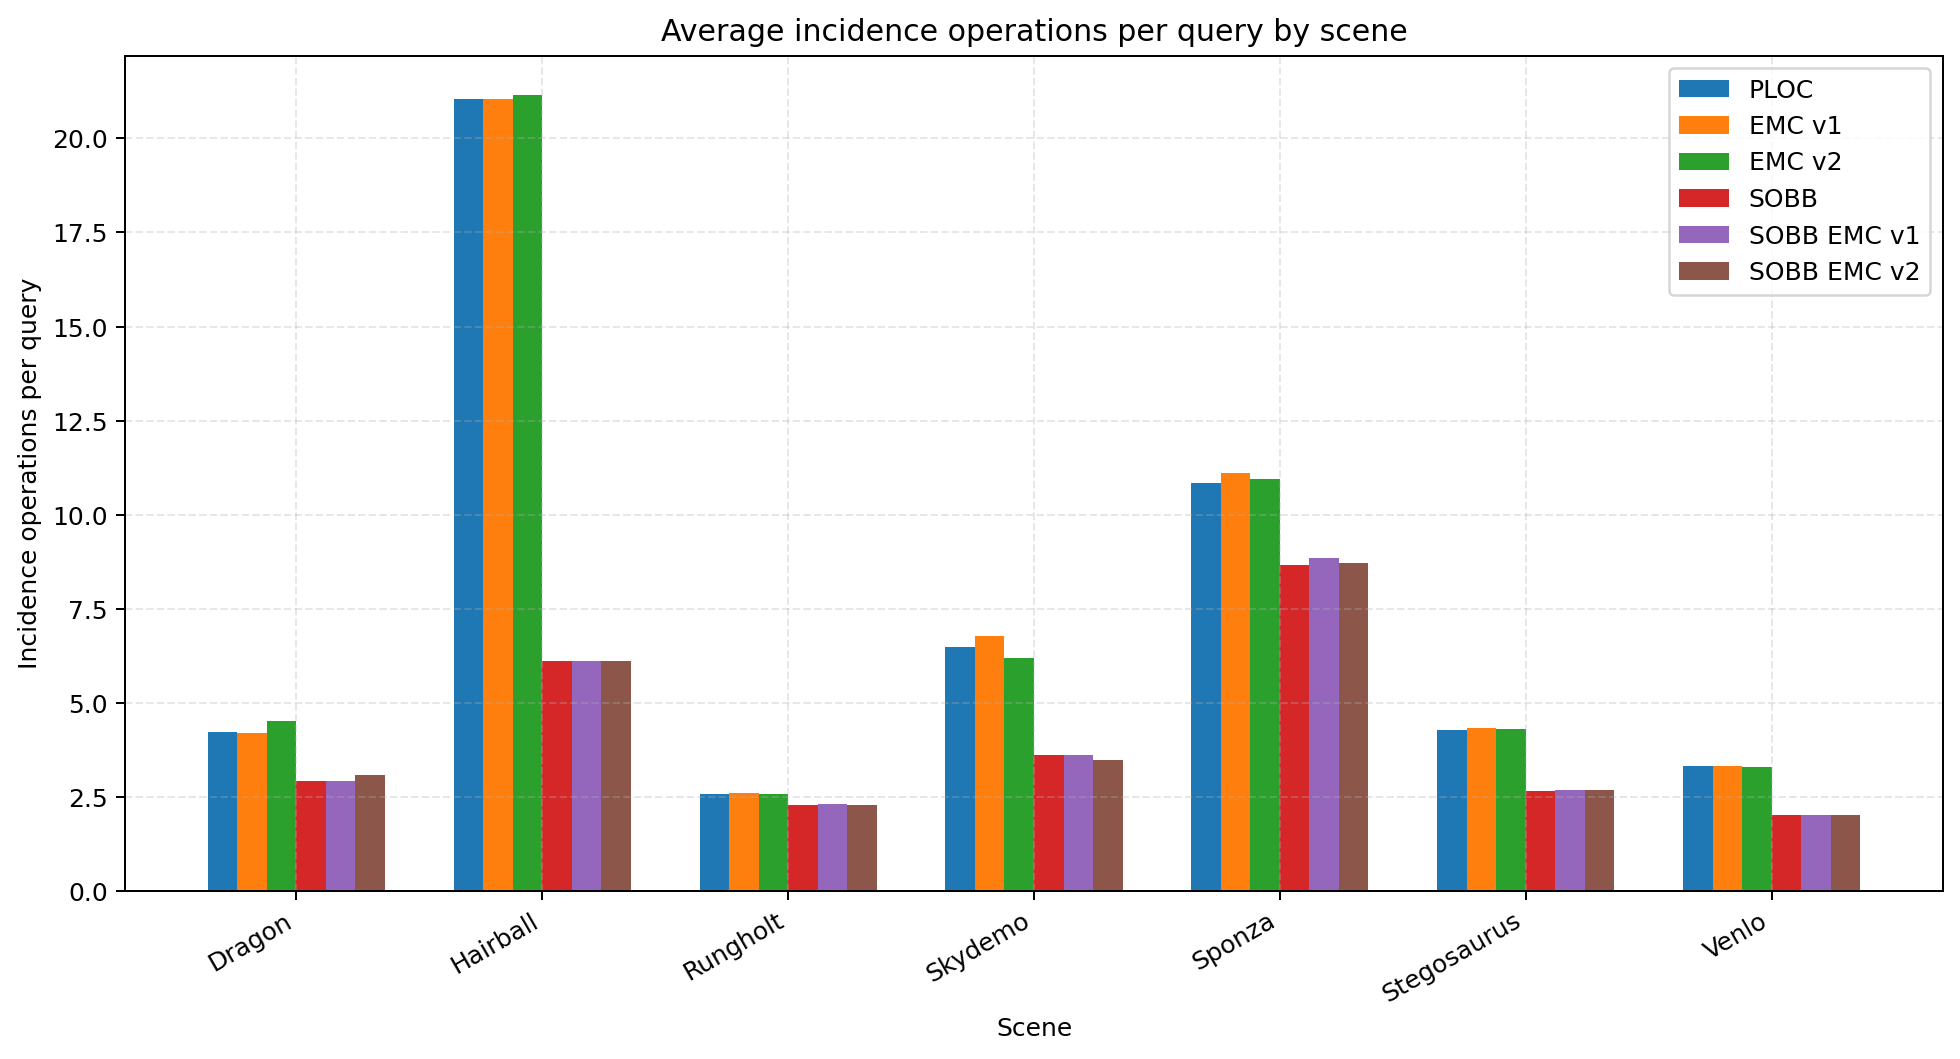
\includegraphics[width=0.95\textwidth]{images/results/rtx3060mobile/graph_scene_incidence_ops_per_query.png}
    \caption{Incidence operation counts of different variants over all scenes. Nvidia RTX 3060 Mobile .}
    \label{fig:incidence-ops-3060}
\end{figure}

\begin{figure}[h!tb]
    \centering
    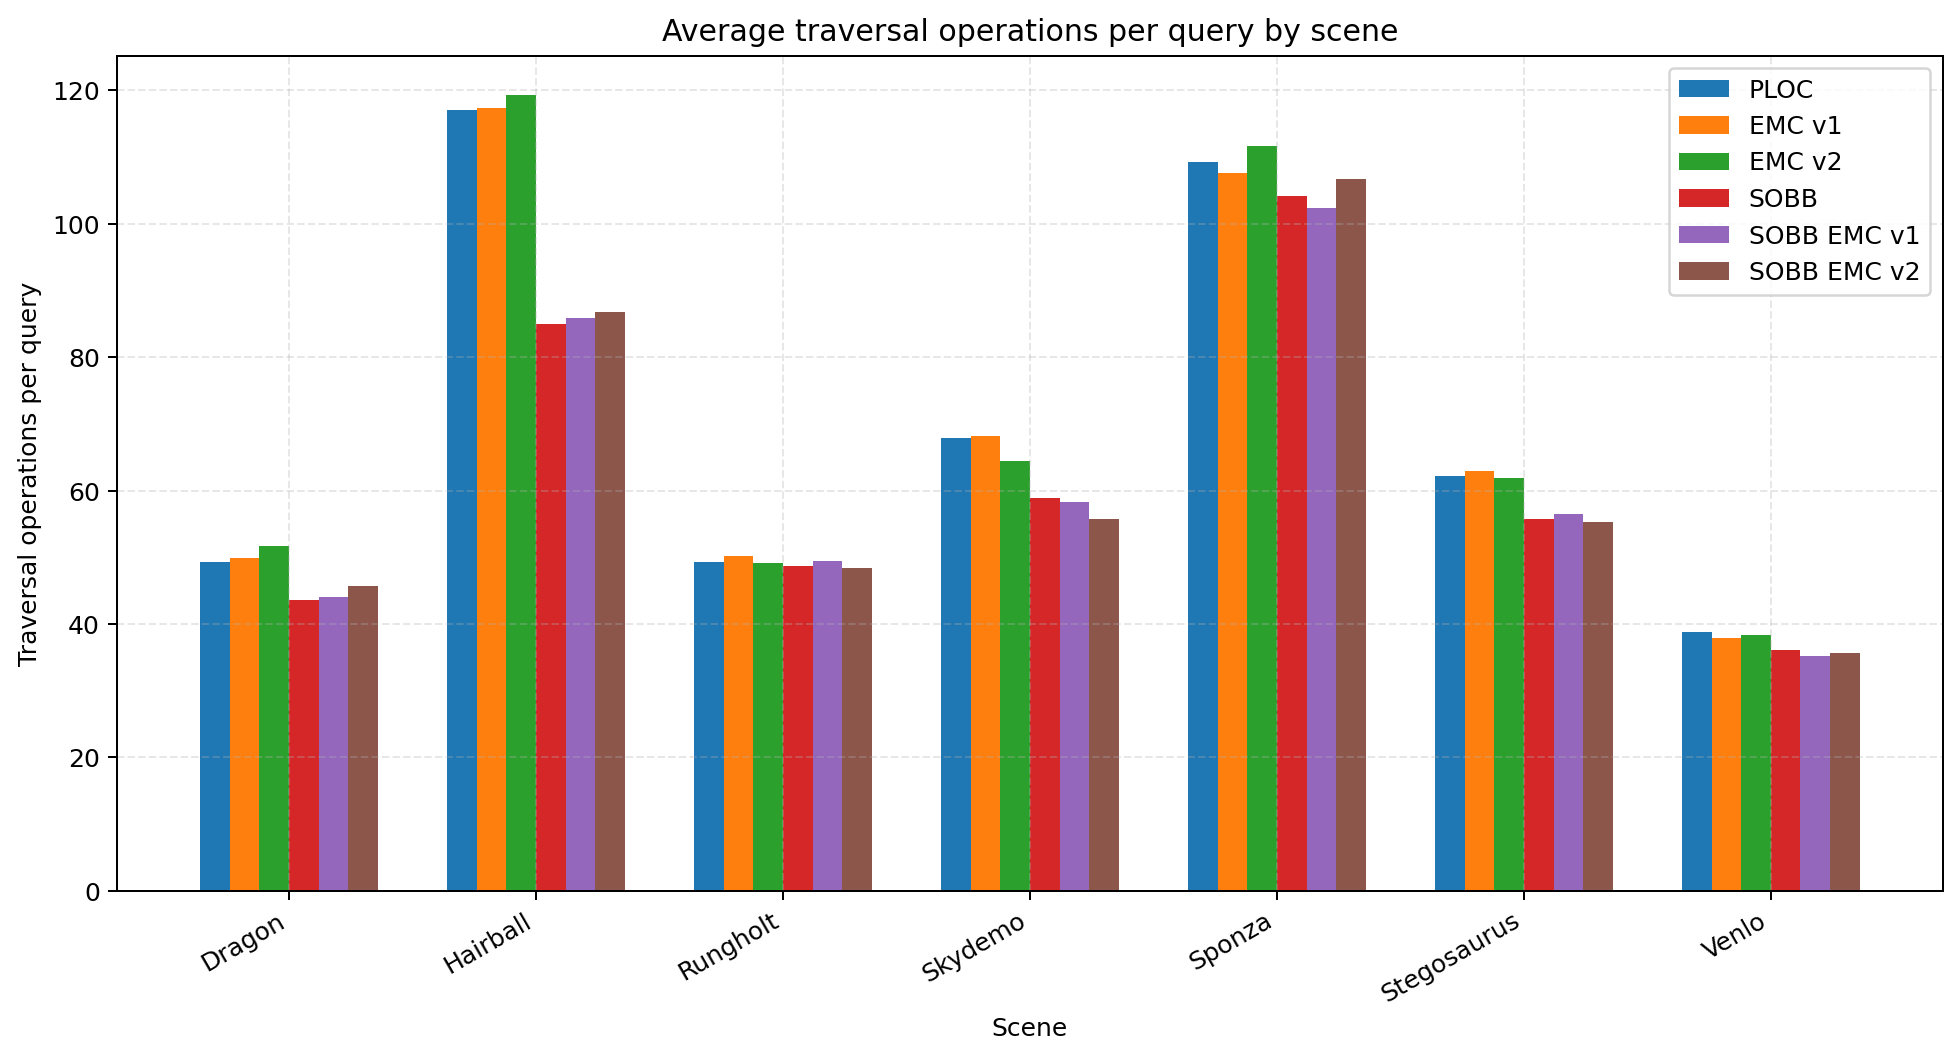
\includegraphics[width=0.95\textwidth]{images/results/rtx3060mobile/graph_scene_traversal_ops_per_query.png}
    \caption{Traversal operation counts of different variants over all scenes. Nvidia RTX 3060 Mobile.}
    \label{fig:traversal-ops-3060}
\end{figure}

\begin{figure}[h!tb]
    \centering
    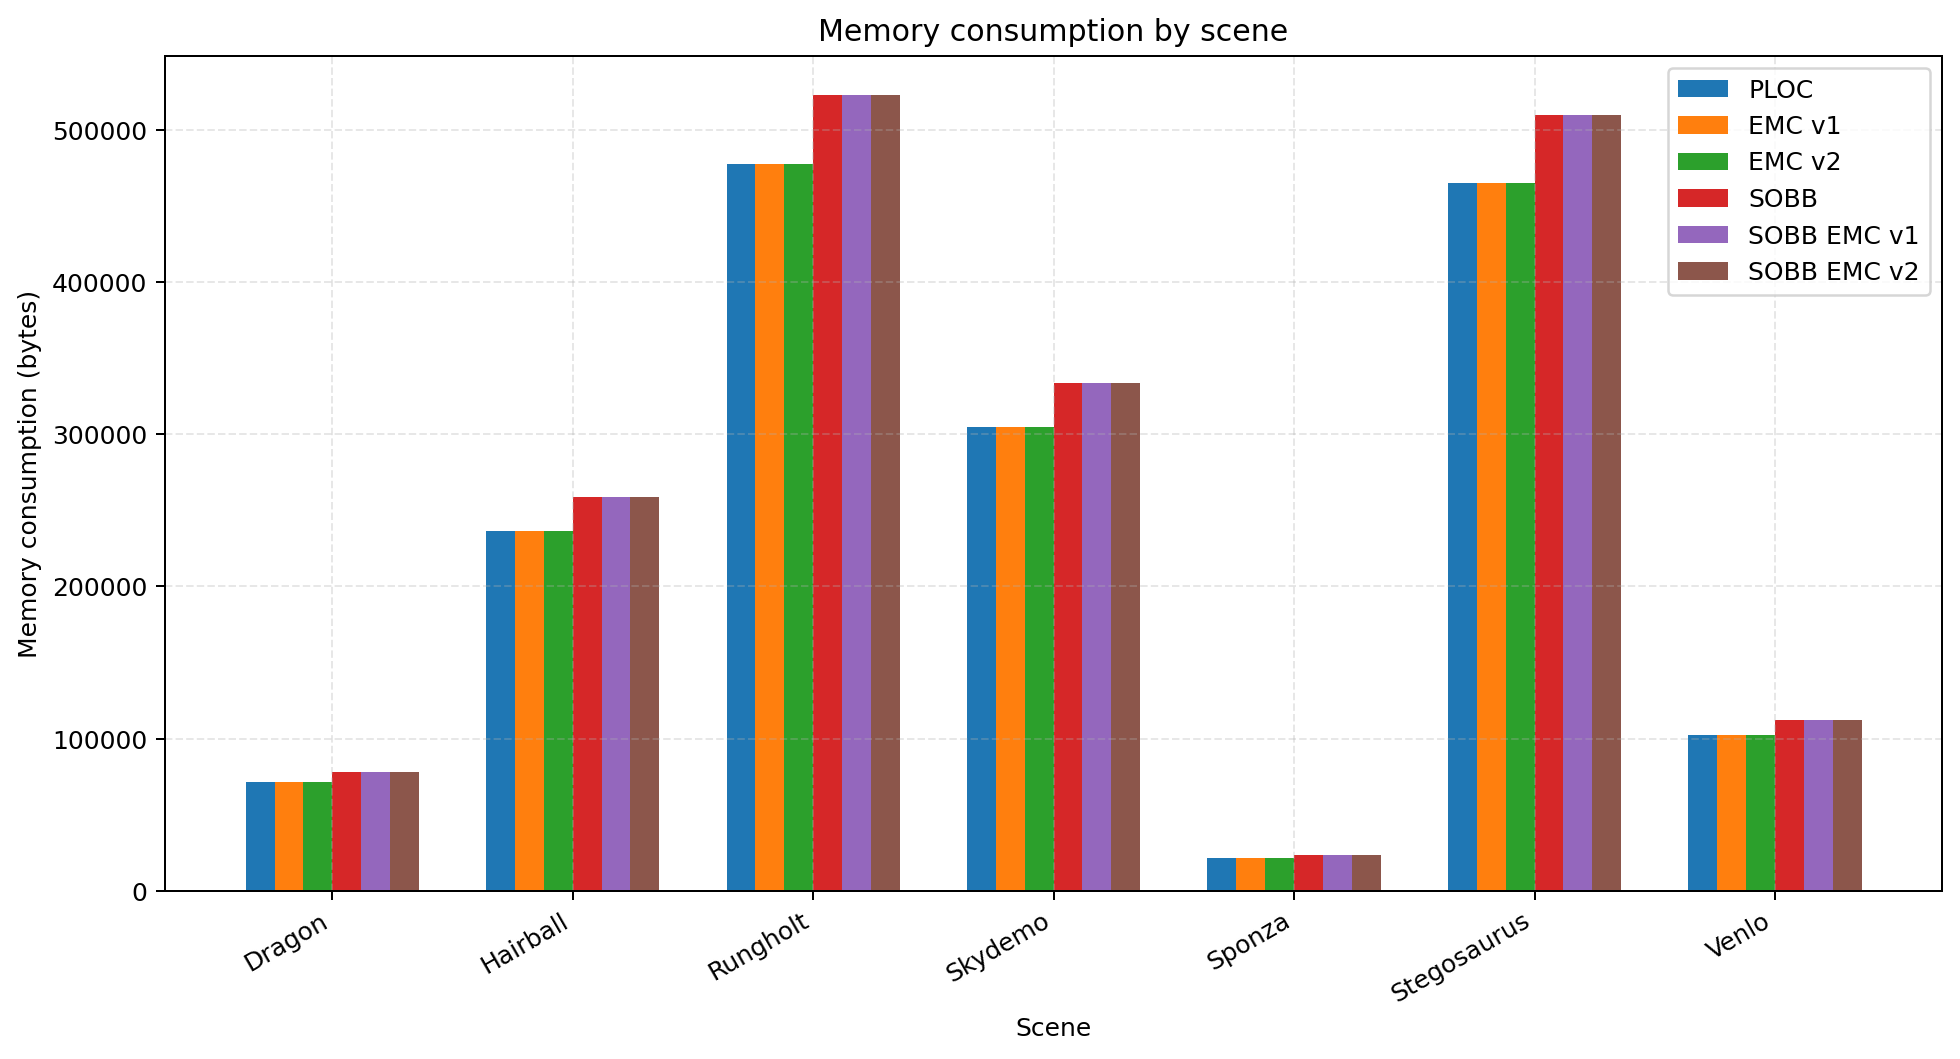
\includegraphics[width=0.95\textwidth]{images/results/rtx3060mobile/graph_scene_memory_consumption.png}
    \caption{Memory consumption of different variants over all scenes. Nvidia RTX 3060 Mobile.}
    \label{fig:memory-consumption-3060}
\end{figure} % include `appendix.tex' from `text/' subdirectory

\backmatter % do not remove this command

\printbibliography % print out the BibLaTeX-generated bibliography list

\chapter{Attachment contents}

\dirtree{%
    .1 /.
    .2 experiments/\DTcomment{ Python benchmark scripts and results }.
    .2 report/\DTcomment{ thesis text, LaTeX source files and other materials }.
    .2 res/\DTcomment{ placeholder scenes }.
    .2 src/\DTcomment{ source code }.
    .2 third-party/\DTcomment{ third party libraries }.
    .2 b.sh\DTcomment{ build script }.
    .2 CMakeLists.txt\DTcomment{ build system configuration }.
    .2 CMakePresets.json\DTcomment{ build presets }.
    .2 Dependencies.cmake\DTcomment{ build system dependencies }.
    .2 r.sh\DTcomment{ run script }.
    .2 README.txt\DTcomment{ short description of the project }.
    .2 license.txt\DTcomment{ thesis license }.
    .2 sample\_config.json\DTcomment{ sample configuration }.
}
 % include `medium.tex' from `text/' subdirectory

\end{document}
